\chapter{Collagen Model}

Having explored the use of the transfer integral method to model DNA, we now turn our attention to the collagen molecule. As with the model of DNA, the collagen model will focus on the shearing force applied to collagen molecule, and study the behaviour of the residue pairs under strain. A major structural difference between the DNA and collagen model is the greater dimensionality that arises from the addition of a third backbone in collagen. Our methodology in calculating the partition function will be similar to that of DNA, hence there will be some common features. 

\section{Collagen Model with a general residue potential}

Starting with a Collagen Model that has a general residue potential we begin with the construction of a Hamiltonian.

\subsection{Construction of the Hamiltonian}

The architecture of the collagen molecule is fairly complex with its triple helix structure. In order to mathematically express this as a Hamiltonian we simplify this structure to one that resembles a triangular prism. This structure retains the important composition of collagen such as the three backbones and residue pairs linking them. Once again we neglect the torsional effects in the triple helix structure and use a potential that is harmonic for small extensions in both the backbone and the pair potentials between the residues. The simplified structure consists of three rows of regularly spaced particles (residues) connected by elastic springs \figref{collagen_model_tri_prism}. The backbone interactions have a spring constant $\kappa$ whereas the residue pair potentials have a spring constant $\kappa'$. The load on the triangular prism structure is applied axially by pulling on one end of the structure while keeping the other end fixed
%
\begin{figure}
\centering 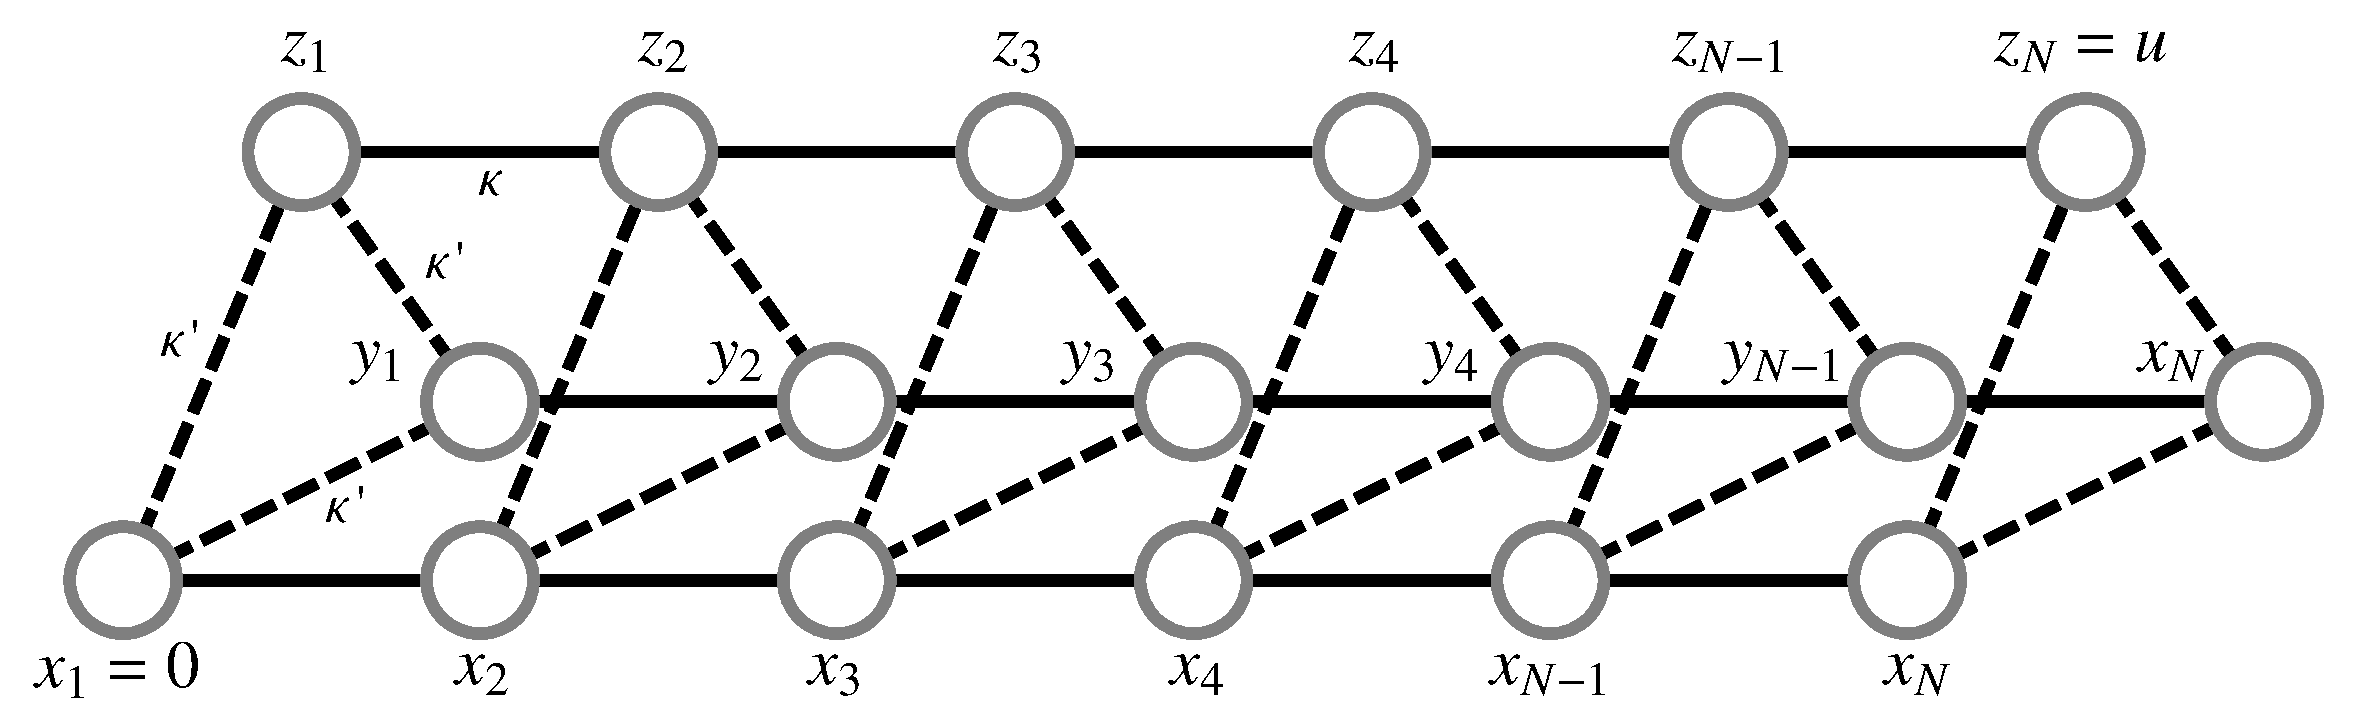
\includegraphics[scale=0.35]{Graphics/Collagen_Model/collagen_structure.pdf}
\caption{Schematic diagram of the collagen model. The thick lines represent the backbones with high spring constants $\kappa$, the dashed lines represent the residue pairs of low spring constant $\kappa'$.}
\label{fig:collagen_model_tri_prism}
\end{figure}
%
in the following way. Each of the three backbones are labelled by $x$, $y$ and $z$, and the positions of particles in each backbone are labelled by $x_i$, $y_i$, and $z_i$. Specifically, we fix the $x$-backbone at $x_{1}=0$ with the opposite end of the structure being pulled on the $z$-backbone by an extension $z_N=u$. The $y$-backbone is free from any external constraints. The partners forming the $i^{th}$ residue pair interact through a general potential $V_{r}\left(\alpha\right)$ which is dependent on the axial pair separations of $(x_{i}-y_{i})$, $(x_{i}-z_{i})$ and $(z_{i}-y_{i})$. For a model with residues at $N$ axial positions the Hamiltonian can be written as 
%
\begin{equation}
\label{collagen_hamiltonian}
H = H_{bb_x} + H_{bb_y} + H_{bb_z}+H_{r}
\end{equation}
%
where
%
\begin{align}
\label{col_hamiltonian_x}
H_{bb_x} &= \sum_{i=1}^{N-1} \frac{1}{2} \kappa \left(x_{i+1}-x_{i} \right)^2 \\
\label{col_hamiltonian_y}
H_{bb_y} &= \sum_{i=1}^{N-1} \frac{1}{2} \kappa \left(y_{i+1}-y_{i} \right)^2 \\
\label{col_hamiltonian_z}
H_{bb_z} &= \sum_{i=1}^{N-1} \frac{1}{2} \kappa \left(z_{i+1}-z_{i} \right)^2 \\
\label{col_hamiltonian_r}
H_{r} &= \sum_{i=1}^{N}V_{r}\left(x_{i}-y_{i}\right)+V_{r}\left(x_{i}-z_{i}\right)+V_{r}\left(z_{i}-y_{i}\right)
\end{align}
%
The separation of variables in the interaction terms is a common 3-body problem in physics where transformations to different co-ordinate systems are used extensively. Drawing similarities to our own Hamiltonian we can apply a transformation that decouples the residue interaction terms in a new co-ordinate system of $R$, $\rho$, and $\lambda$. We make the following transformations
%
\begin{align}
\label{col_trans}
R_{i}&=\frac{1}{\sqrt{3}}(x_{i}+y_{i}+z_{i})\\
\rho_{i}&=\frac{1}{\sqrt{2}}(x_{i}-y_{i})\\
\lambda_{i}&=\frac{1}{\sqrt{6}}(x_{i}+y_{i}-2z_{i})
\end{align}
%
In terms of the original co-ordinate system we have
%
\begin{align}
\label{col_x}
x_{i}&=\frac{R_{i}}{\sqrt{3}} + \frac{\rho_{i}}{\sqrt{2}} + \frac{\lambda_{i}}{\sqrt{6}}\\
\label{col_y}
y_{i}&=\frac{R_{i}}{\sqrt{3}} - \frac{\rho_{i}}{\sqrt{2}} + \frac{\lambda_{i}}{\sqrt{6}}\\
\label{col_z}
z_{i}&=\frac{R_{i}}{\sqrt{3}} - \sqrt{\frac{2}{3}}\lambda_{i}
\end{align}
%
Hence the new Hamiltonian may be written as a function of $\vec{R}$, $\vec{\rho}$ and $\vec{\lambda}$
%
\begin{equation}\label{col_ham_trans1}
\begin{split}
H &= \sum_{i=1}^{N-1} \frac{\kappa}{2}\left(R_i-R_{i+1}\right)^{2}+\frac{\kappa}{2}\left(\rho_i-\rho_{i+1}\right)^{2}+\frac{\kappa}{2}\left(\lambda_i-\lambda_{i+1}\right)^{2} \\ 
&+\sum_{i=1}^{N}V_{r}\left(\sqrt{2}\rho_i\right)+V_{r}\left(\frac{\rho_i-\sqrt{3}\lambda}{\sqrt{2}}\right)+V_{r}\left(\frac{\sqrt{3}\lambda-\rho_i}{\sqrt{2}}\right)
\end{split}
\end{equation}
%
\subsection{Partition Function Integral}
%
The partition function is evaluated using the same partition function integral method already employed in the DNA Model. As we have transformed the co-ordinate system to the new co-ordinates $R$, $\rho$ and $\lambda$ we can ensure that integration over phase-space is also transformed correctly by calculating the Jacobian matrix of \eqref{col_x}, \eqref{col_y} and \eqref{col_z}. Transforming the integration over phase-space we have
%
\begin{equation}
\int\,d\tau=\iiint\,dxdydz=\iiint\,JdRd\rho d\lambda 
\end{equation}
%
where 
\begin{equation}
J(R,\rho,\lambda) = \begin{vmatrix}
\frac{\partial x}{\partial R} & \frac{\partial x}{\partial \rho} & \frac{\partial x}{\partial \lambda}\\
\frac{\partial y}{\partial R} & \frac{\partial y}{\partial \rho} & \frac{\partial y}{\partial \lambda}\\
\frac{\partial z}{\partial R} & \frac{\partial z}{\partial \rho} & \frac{\partial z}{\partial \lambda}
\end{vmatrix}
= \begin{vmatrix}
\frac{1}{\sqrt{3}} & \frac{1}{\sqrt{2}} & \frac{1}{\sqrt{6}}\\
\frac{1}{\sqrt{3}} & -\frac{1}{\sqrt{2}} & \frac{1}{\sqrt{6}}\\
\frac{1}{\sqrt{3}} & 0 & \sqrt{\frac{2}{3}}
\end{vmatrix}
=1
\end{equation}
%
With new variables converted into dimensionless quantities using
%
\begin{align}
\label{col_dimensionless_quantities}
R&\rightarrow R\left(\frac{\kappa \beta}{2}\right)^{-\frac{1}{2}}\\
\rho&\rightarrow \rho\left(\frac{\kappa \beta}{2}\right)^{-\frac{1}{2}}\nonumber\\
\lambda&\rightarrow \lambda\left(\frac{\kappa \beta}{2}\right)^{-\frac{1}{2}}\nonumber
\end{align}
%
the Hamiltonian becomes
%
\begin{align}\label{col_ham_trans2}
\beta H &= \sum_{i=1}^{N-1}\left(R_i-R_{i+1}\right)^{2}+\left(\rho_i-\rho_{i+1}\right)^{2}+\left(\lambda_i-\lambda_{i+1}\right)^{2} \nonumber\\ 
&+\sum_{i=1}^{N}\beta\,V_{r}\left(\frac{2\rho_i}{\left( \beta \kappa\right)^{\frac{1}{2}}}\right)+\beta\,V_{r}\left(\frac{\rho_i+ \sqrt{3}\lambda_i}{\left( \beta \kappa\right)^{\frac{1}{2}}}\right)+\beta\,V_{r}\left(\frac{\sqrt{3}\lambda_i - \rho_i}{\left( \beta \kappa\right)^{\frac{1}{2}}}\right)
\end{align}
%
Making the variables dimensionless introduces a constant factor to the partition integral which we can ignore. The partition function integral before the imposition of boundary constraints becomes
%
\begin{equation}\label{col_part_int}
Z=\int \prod_{i=1}^{N}\,dR_{i}\,d\rho_{i}\,d\lambda _{i}\exp\left(-\beta H\left(R_{i},\rho_{i},\lambda_{i}\right)\right)
\end{equation}
%
\subsection{Transfer Matrices}

The transfer matrices are found by rewriting the exponential terms of the partition function integral. Inserting the Hamiltonian equation \eqref{col_ham_trans2} into \eqref{col_part_int}, the exponential terms become
%
\begin{align}\label{col_hyp_expo_term1}
\exp\left(-\beta H\right)&=\prod_{i=1}^{N-1}\exp\left(-\left(R_{i+1}-R_{i}\right)^{2}\right)\prod_{j=1}^{N-1}\exp\left(-\left(\rho_{j+1}-\rho_{j}\right)^{2}\right)\nonumber\\
&\times\prod_{k=1}^{N-1}\exp\left(-\left(\lambda_{k+1}-\lambda_{k}\right)^{2}\right)\prod_{l=1}^{N}\exp\left(-V\left(\rho_{l},\lambda_{l}\right)\right)
\end{align}
%
Where
%
\begin{equation}
V\left(\rho_{l},\lambda_{l}\right)  = \beta\,V_{r}\left(\frac{2\rho_l}{\left( \beta \kappa\right)^{\frac{1}{2}}}\right)+\beta\,V_{r}\left(\frac{\rho_l+ \sqrt{3}\lambda_l}{\left( \beta \kappa\right)^{\frac{1}{2}}}\right)+\beta\,V_{r}\left(\frac{\sqrt{3}\lambda_l - \rho_l}{\left( \beta \kappa\right)^{\frac{1}{2}}}\right)
\end{equation}
%
The combination of the two variables in the potential $V_{r}$ requires us to create a transfer matrix that is a function of both $\rho$ and $\lambda$. By factorising the products and keeping the terms symmetric in $R$, $\rho$ and $\lambda$, the exponential terms can be written as 
%
\begin{equation}\label{col_hyp_expo_term2}
\begin{split}
\exp\left(-\beta H\right)&=\prod_{i=1}^{N-1}\exp\left(-\left(R_{i+1}-R_{i}\right)^{2}\right) \\
&\times\prod_{j=1}^{N-1}\left[\exp\left(-\left(\rho_{j+1}-\rho_{j}\right)^2\right)\exp\left(-\left(\lambda_{j+1}-\lambda_{j}\right)^2\right)\exp\left(-\frac{V\left(\rho_{j},\lambda_{j}\right)}{2}\right)\right. \\
&\times\left.\exp\left(-\frac{V\left(\rho_{j+1},\lambda_{j+1}\right)}{2}\right)\right]\exp\left(-\frac{V\left(\rho_{1},\lambda_{1}\right)}{2}\right)\exp\left(-\frac{V\left(\rho_{N},\lambda_{N}\right)}{2}\right)
\end{split}
\end{equation}
%
The similarities between the exponentials in \eqref{dna_rearranged_expo} and \eqref{col_hyp_expo_term2} mean that we can use \eqref{dna_tm_xi} for the transfer matrices in $R$. The two variable potential $V\left(\rho,\lambda\right)$ requires a different type of transfer matrix that might be termed a general transfer hyper-matrix. 
%
\begin{equation}\label{col_hyp_trans_R}
T_{R}\left(R,R'\right) = \exp\left(-\left(R-R'\right)^2\right)
\end{equation}
%
\begin{equation}\label{col_hyp_trans_rho_lambda}
\begin{split}
\hat{T}_{\rho\lambda}\left(\rho,\lambda,\rho',\lambda'\right) = \exp\left(-\left(\rho-\rho'\right)^2\right)\exp\left(-\left(\lambda-\lambda'\right)^2\right)\exp\left(-\left(\frac{V\left(\rho,\lambda\right)+V\left(\rho',\lambda'\right)}{2}\right)\right)
\end{split}
\end{equation}
%
The four variable $\hat{T}_{\rho\lambda}$ transfer hyper-matrix arises because of the inseparable nature of the two variables $\rho$ and $\lambda$ when we consider a general potential $V_{r}\left(\rho,\lambda\right)$. We demonstrate in the following chapter that the terms do separate when we use a harmonic potential. Using these transfer matrices the partition function integral for a general residue pair potential becomes
%
\begin{align}\label{col_hyp_part_int}
Z=&\int\prod^{N}_{k=1}dR_k\,d\rho_k\,d\lambda_k\prod^{N-1}_{i=1}T_{R}(R_i,R_{i+1})\prod^{N-1}_{j=1}\hat{T}_{\rho\lambda}(\rho_j,\lambda_j,\rho_{j+1},\lambda_{j+1})\nonumber \\
&\times\exp\left(-\frac{V\left(\rho_{1},\lambda_{1}\right)}{2}\right)\exp\left(-\frac{V\left(\rho_{N},\lambda_{N}\right)}{2}\right)
\end{align}
%
Residue pair breakage descriptions introduced as $g$ factors into the transfer matrices will not be included into the collagen model. We find that  doing so makes the mathematics for contracting the transfer matrices extremely difficult. Instead we follow Peyrard et al. and describe breakage by using an anharmonic residue pair potential. The collagen model will be developed for an intact state.

\subsection{Boundary Conditions}

Delta functions are used to impose the external constraints on the collagen backbones. Because we have an ancillary $y$ backbone in the model, a refinement is needed to the delta function at the fixed end where $x_{1}=0$ that correctly describes the behaviour of a shearing force. In order to exploit the symmetry of the collagen structure both the $x$, and $z$ backbones are extended by $u/2$ using the delta functions $\delta\left(x_1+\frac{u}{2}\right)$ and $\delta\left(z_N-\frac{u}{2}\right)$. 
%
\begin{equation}\label{col_hyp_bound_cond}
\delta\left(x_1+\frac{u}{2}\right)\delta\left(z_N-\frac{u}{2}\right) = \delta\left(\frac{R_1}{\sqrt{3}} + \frac{\rho_1}{\sqrt{2}} + \frac{\lambda_1}{\sqrt{6}}+\frac{u}{2}\right)\delta\left(\frac{R_N}{\sqrt{3}} - \sqrt{\frac{2}{3}}\lambda_N-\frac{u}{2}\right) 
\end{equation}
%
An additional integral over a delta function  $\int\,d\rho'_N \delta\left(\rho'_N-\rho_N\right)$ is introduced into the partition integral to aid the contraction of the $\hat{T}_{\rho\lambda}$ transfer matrices. The full set of inserted boundary conditions now become
%
\begin{equation}\label{col_hyp_full_boundcond}
\int d\rho'_N\, \delta\left(\frac{R_1}{\sqrt{3}} + \frac{\rho_1}{\sqrt{2}} + \frac{\lambda_1}{\sqrt{6}}+\frac{u}{2}\right)\delta\left(\frac{R_N}{\sqrt{3}} - \sqrt{\frac{2}{3}}\lambda_N-\frac{u}{2}\right)  \delta\left(\rho'_N-\rho_N\right)
\end{equation}
%
which is to be inserted into the integrand in the expression for the partition function.
%
\subsection{Eigenvalue Equations}

From the Hamiltonian \eqref{col_ham_trans1} we can draw some parallels with the DNA model. The backbone in both models have same harmonic behaviour in each strand determined by a stiffness constant $\kappa$  leading to identical backbone transfer matrices. This allows us to use the same form of the eigenfunction used to contract the backbone transfer matrices in DNA. Differences arise in general potential terms where different eigenfunctions for the residue pairs need to be calculated. However, we will see later that for a harmonic residue pair potential we can in fact use the same form of the base-pair eigenfunction from DNA for the special case where $\eta_b \rightarrow \infty$ for an intact structure.

The boundary condition delta functions are expanded as a set of normalised eigenfunctions of the transfer matrices satisfying equations \eqref{col_hyp_trans_R}, and \eqref{col_hyp_trans_rho_lambda}. The expansion gives
%
\begin{align}
\label{col_hyp_bc_r}
\delta\left(\frac{R_1}{\sqrt{3}} + \frac{\rho_1}{\sqrt{2}} + \frac{\lambda_1}{\sqrt{6}}+\frac{u}{2}\right)&=\sum_{l_R}\psi_{l_R}\left(\frac{\lambda_1 + \sqrt{3}\rho_1}{\sqrt{2}}\right)\psi_{l_R}\left(R_{1}+\frac{u}{2}\sqrt{3}\right)\nonumber\\
&=\sum_{l_R}\psi_{l_R}\left(\frac{\lambda_1 + \sqrt{3}\rho_1}{\sqrt{2}}\right)\psi_{l_R}\left(R_{1}\right)\exp\left(\frac{il_R\sqrt{3}\pi u}{L}\right)
\end{align}
%
\begin{equation}
\label{col_hyp_bc_rho_lambda}
\delta\left(\rho'_N-\rho_N\right)\delta\left(\frac{R_N}{\sqrt{3}} - \sqrt{\frac{2}{3}}\lambda_N-\frac{u}{2}\right)=\sum_{l_{\rho\lambda}}\hat{\psi}^{*}_{l_{\rho\lambda}}\left(\rho_{N},\lambda_{N}\right)\hat{\psi}_{l_{\rho\lambda}}\left(\rho'_{N},\frac{R_N-\frac{u}{2}\sqrt{3}}{\sqrt{2}}\right)
\end{equation}
%
where the eigenvalue equations for $\psi_{l_{R}}$ and $\hat{\psi}_{l_{\rho\lambda}}$ are
%
\begin{equation}\label{col_hyp_eign_l_r}
\int dR'\,T_{R}\left(R,R'\right)\psi_{l_{R}}\left(R'\right) = \Lambda_{l_{R}}\psi_{l_{R}}\left(R\right)
\end{equation}
%
\begin{equation}\label{col_hyp_eign_l_rho_lambda}
\iint d\rho'd\lambda'\,\hat{T}_{\rho\lambda}\left(\rho,\lambda,\rho',\lambda'\right)\hat{\psi}_{l_{\rho\lambda}}\left(\rho',\lambda'\right) = \hat{\Lambda}_{l_{\rho\lambda}}\hat{\psi}_{l_{\rho\lambda}}\left(\rho,\lambda\right)
\end{equation}
%
For the eigenfunctions $\psi_{l_{R}}$ the transfer matrix $T_{R}\left(R,R'\right)$ is identical to \eqref{dna_tm_xi}, and therefore we can use the analytical eigenfunctions calculated already, $\psi_{l_R}\left(\alpha\right)=L^{-\frac{1}{2}}\exp(is2\pi \alpha/L)$ (\eqref{dna_T_eigenfunction}). The transfer matrix in \eqref{col_hyp_eign_l_rho_lambda} is in fact an eigenproblem expressed in terms of an operator acting on a matrix rather than on a vector.
%
\subsection{Transfer Matrix Method}
%
Inserting the boundary conditions \eqref{col_hyp_bc_r} and \eqref{col_hyp_bc_rho_lambda} to the partition function integral \eqref{col_hyp_part_int} we get
%
\begin{align}\label{col_hyp_part_1}
Z \left(u\right)&=\int\prod^{N}_{i=1}dR_i\,d\rho_i\,d\lambda_i\prod^{N-1}_{j=1}T_{R}(R_j,R_{j+1})\prod^{N-1}_{k=1}\hat{T}_{\rho\lambda}(\rho_k,\lambda_k,\rho_{k+1},\lambda_{k+1})\nonumber\\
&\times\exp\left(-\frac{V\left(\rho_{1},\lambda_{1}\right)}{2}\right)\exp\left(-\frac{V\left(\rho_{N},\lambda_{N}\right)}{2}\right)\nonumber\\
&\times\int d\rho'_N\,\sum_{l_R}\psi_{l_R}\left(\frac{\lambda_1 + \sqrt{3}\rho_1}{\sqrt{2}}\right)\psi_{l_R}\left(R_{1}\right)\exp\left(\frac{il_R\sqrt{3}\pi u}{L}\right)\nonumber\\ 
&\times\sum_{l_{\rho\lambda}}\hat{\psi}^{*}_{l_{\rho\lambda}}\left(\rho_{N},\lambda_{N}\right)\hat{\psi}_{l_{\rho\lambda}}\left(\rho'_{N},\frac{R_N-\frac{u}{2}\sqrt{3}}{\sqrt{2}}\right)
\end{align}

%
We can easily contract the $T_R$ transfer matrices with the eigenfunctions $\psi_{l_R}\left(R_{1}\right)$ up to $\psi_{l_R}\left(R_{N}\right)$ to give
%
\begin{align}\label{col_hyp_part_2}
Z \left(u\right)&=\sum_{l_R,l_{\rho\lambda}}\Lambda_{l_{R}}^{N-1}\exp\left(\frac{il_{R}\sqrt{3}\pi u}{L}\right)\int\prod^{N}_{i=1}\,d\rho_i\,d\lambda_i\prod^{N-1}_{j=1}\hat{T}_{\rho\lambda}(\rho_j,\lambda_j,\rho_{j+1},\lambda_{j+1})\nonumber\\
&\times\iint dR_N\,d\rho'_N\,\psi_{l_R}\left(R_{N}\right)\exp\left(-\frac{V\left(\rho'_{N},\lambda_N\right)}{2}\right)\hat{\psi}_{l_{\rho\lambda}}\left(\rho'_{N},\frac{R_N-\frac{u}{2}\sqrt{3}}{\sqrt{2}}\right)\nonumber\\
&\times\,\hat{\psi}^{*}_{l_{\rho\lambda}}\left(\rho_{N},\lambda_{N}\right)\exp\left(-\frac{V\left(\rho_{1},\lambda_{1}\right)}{2}\right)\psi_{l_R}\left(\frac{\lambda_1 + \sqrt{3}\rho_1}{\sqrt{2}}\right)
\end{align}
%
We can use the eigenfunction $\hat{\psi}^{*}_{l_{\rho\lambda}}\left(\rho_{N},\lambda_{N}\right)$ to contract the $\hat{T}_{\rho\lambda}$ transfer matrices. The delta function introduced in \eqref{col_hyp_bc_rho_lambda} allow us to write $\rho_{N}=\rho'_{N}$ and $\lambda_{N}=\frac{R_N-\frac{u}{2}\sqrt{3}}{\sqrt{2}}$ in $V(\rho_{N},\lambda_{N})$.
%
\begin{equation}\label{col_hyp_part_3}
\begin{split}
Z\left(u\right)&=\sum_{l_R,l_{\rho\lambda}}\Lambda_{l_{R}}^{N-1}\hat{\Lambda}_{l_{\rho\lambda}}^{N-1}\exp\left(\frac{il_R\sqrt{3}\pi u}{L}\right)\\
\times&\iint dR_N\,d\rho'_N\,\psi_{l_R}\left(R_{N}\right)\exp\left(-\frac{V\left(\rho'_{N},\frac{R_N-\frac{u}{2}\sqrt{3}}{\sqrt{2}}\right)}{2}\right)\hat{\psi}_{l_{\rho\lambda}}\left(\rho'_{N},\frac{R_N-\frac{u}{2}\sqrt{3}}{\sqrt{2}}\right)\\
\times&\iint d\rho_1d\lambda_1\,\hat{\psi}^{*}_{l_{\rho\lambda}}\left(\rho_{1},\lambda_{1}\right)\exp\left(-\frac{V\left(\rho_{1},\lambda_{1}\right)}{2}\right)\psi_{l_R}\left(\frac{\lambda_1 + \sqrt{3}\rho_1}{\sqrt{2}}\right)
\end{split}
\end{equation}
%
Here we make a change of variable such that
%
\begin{equation}\label{variable_change}
\tilde{R}_{N}=\frac{R_N-\frac{u}{2}\sqrt{3}}{\sqrt{2}}
\end{equation}
%
Ignoring the constants outside the sum the partition function now becomes
%
\begin{align}\label{col_hyp_part_final}
Z\left(u\right)&=\sum_{l_R,l_{\rho\lambda}}\Lambda_{l_{R}}^{N-1}\hat{\Lambda}_{l_{\rho\lambda}}^{N-1}\exp\left(\frac{il_R2\sqrt{3}\pi u}{L}\right)\nonumber\\
&\times\iint d\tilde{R}_N\,d\rho'_N\,\psi_{l_R}\left(\sqrt{2}\tilde{R}_{N}\right)\exp\left(-\frac{V\left(\rho'_{N},\tilde{R}_{N}\right)}{2}\right)\hat{\psi}_{l_{\rho\lambda}}\left(\rho'_{N},\tilde{R}_{N}\right)\nonumber\\
&\times\iint d\rho_1d\lambda_1\,\hat{\psi}^{*}_{l_{\rho\lambda}}\left(\rho_{1},\lambda_{1}\right)\exp\left(-\frac{V\left(\rho_{1},\lambda_{1}\right)}{2}\right)\psi_{l_R}\left(\frac{\lambda_1 + \sqrt{3}\rho_1}{\sqrt{2}}\right)
\end{align}
%
\subsection{Mean Axial Displacement}
%
The calculation of the mean axial displacement of various components in the collagen model is rather different to DNA where it was the average of the base-pair $(x_{i}-y_{i})$ separation. 
The third backbone in the collagen model adds another variable to the mean axial displacement calculation where the average axial separation is now the difference between the mid-point of the $xz_{i}$ residue pair and the position of the $y_{i}$ residue in the $i^{th}$ segment of the structure, that is, $\frac{x_{i}+z_{i}}{2}-y_{i}$. Let us define the mean axial displacement to be $\zeta$, where
%
\begin{equation}
\label{col_mxd}
\langle\zeta_\alpha\rangle = \langle x_\alpha+z_\alpha-2y_\alpha\rangle
\end{equation}
%
and $\alpha$ is a segment label in the range 1 to $N$. Transforming this to the $R\rho\lambda$ co-ordinate system we use \eqref{col_x}, \eqref{col_y} and \eqref{col_z} to get
%
\begin{equation}
\label{col_mxd2}
\langle\zeta_{\alpha}\rangle = \frac{-\sqrt{3}\langle\lambda_{\alpha}\rangle+3\langle\rho_{\alpha}\rangle}{\sqrt{\beta\kappa}}
\end{equation}
%
We therefore need to calculate $\langle\lambda_\alpha\rangle$ and $\langle\rho_\alpha\rangle$ to find the mean axial displacements for the collagen model. These equations are similar to \eqref{dna_mxd_eta} where
%
\begin{equation}
\label{col_mxd_rho}
\langle\rho_{\alpha}\rangle=\frac{\int \prod^{N}_{i=1}dR_{i}d\rho_{i}d\lambda_{i}\,\rho_{\alpha}\exp\left(-\beta H\left(R_{i},\rho_{i},\lambda_{i}\right)\right)B_c}{\int \prod^{N}_{i=1}dR_{i}d\rho_{i}d\lambda_{i}\,\exp\left(-\beta H\left(R_{i},\rho_{i},\lambda_{i}\right)\right)B_c}
\end{equation}
%
and
%
\begin{equation}
\label{col_mxd_lambda}
\langle\lambda_{\alpha}\rangle=\frac{\int \prod^{N}_{i=1}dR_{i}d\rho_{i}d\lambda_{i}\,\lambda_{\alpha}\exp\left(-\beta H\left(R_{i},\rho_{i},\lambda_{i}\right)\right)B_c}{\int \prod^{N}_{i=1}dR_{i}d\rho_{i}d\lambda_{i}\,\exp\left(-\beta H\left(R_{i},\rho_{i},\lambda_{i}\right)\right)B_c}
\end{equation}
%
The boundary conditions that apply constraints to the collagen structure from \eqref{col_hyp_full_boundcond} are contained within $B_c$. With the partition function already calculated we are left with evaluating the following two integrals to find the mean axial displacement
%
\begin{equation}
\label{col_mxd_z_rho}
Z_{\rho_\alpha}=\iiint \prod^{N}_{i=1}dR_{i}d\rho_{i}d\lambda_{i}\,\rho_{\alpha}\exp\left(-\beta H\left(R_{i},\rho_{i},\lambda_{i}\right)\right)B_c
\end{equation}
%
\begin{equation}
\label{col_mxd_z_lambda}
Z_{\lambda_\alpha}=\iiint \prod^{N}_{i=1}dR_{i}d\rho_{i}d\lambda_{i}\,\lambda_{\alpha}\exp\left(-\beta H\left(R_{i},\rho_{i},\lambda_{i}\right)\right)B_c
\end{equation}
%
\subsection{Calculation of average $\rho_{\alpha}$ and $\lambda_{\alpha}$}
%
We begin with $Z_{\lambda_{\alpha}}$, and continue from \eqref{col_hyp_part_1} where the transfer matrices in $R$ have already been contracted. A modification of this partition function is needed to include the variable $\lambda_{\alpha}$
%
\begin{equation}\label{col_hyp_mxd_z_lambda1}
\begin{split}
Z_{\lambda_{\alpha}}&\left(u\right)=\sum_{l_R,l_{\rho\lambda}}\Lambda_{l_{R}}^{N-1}\exp\left(\frac{il_{R} 2\sqrt{3}\pi u}{L}\right)\iint\prod^{N}_{i=1}\,d\rho_i\,d\lambda_i \hat{T}_{\rho\lambda}(\rho_1,\lambda_1,\rho_2,\lambda_2)...\\
&\times\hat{T}_{\rho\lambda}(\rho_{\alpha-1},\lambda_{\alpha-1},\rho_\alpha,\lambda_\alpha) \lambda_{\alpha}\hat{T}_{\rho\lambda}(\rho_\alpha,\lambda_\alpha,\rho_{\alpha+1},\lambda_{\alpha+1})...\hat{T}_{\rho\lambda}(\rho_{N-1},\lambda_{N-1},\rho_N,\lambda_N)\\
&\times\iint d\tilde{R}_N d\rho'_N\psi_{l_R}\left(\sqrt{2}\tilde{R}_N\right)\exp\left(-\frac{V\left(\rho'_{N},\tilde{R}_N\right)}{2}\right)\hat{\psi}_{l_{\rho\lambda}}\left(\rho'_{N},\tilde{R}_N\right)\\
&\times\hat{\psi}^{*}_{l_{\rho\lambda}}\left(\rho_{N},\lambda_{N}\right)\exp\left(-\frac{V\left(\rho_{1},\lambda_{1}\right)}{2}\right)\psi_{l_R}\left(\frac{\lambda_1 + \sqrt{3}\rho_1}{\sqrt{2}}\right)
\end{split}
\end{equation}
%
We can start from the eigenfunction $\hat{\psi}^{*}_{l_{\rho\lambda}}\left(\rho_{N},\lambda_{N}\right)$ to contract the $\hat{T}_{\rho\lambda}$ transfer matrices down to $\hat{\psi}^{*}_{l_{\rho\lambda}}\left(\rho_{\alpha},\lambda_{\alpha}\right)$
%
\begin{align}
\label{col_hyp_mxd_z_lambda2}
Z_{\lambda_{\alpha}}& \left(u\right)=\sum_{l_R,l_{\rho\lambda}}\Lambda_{l_{R}}^{N-1}\Lambda_{l_{\rho\lambda}}^{N-\alpha}\exp\left(\frac{i2\sqrt{3}l_R\pi u}{L}\right)\nonumber\\
&\times\iint d\tilde{R}_N d\rho'_N\psi_{l_R}\left(\sqrt{2}\tilde{R}_N\right)\exp\left(-\frac{V\left(\rho'_{N},\tilde{R}_N\right)}{2}\right)\hat{\psi}_{l_{\rho\lambda}}\left(\rho'_{N},\tilde{R}_N\right)\nonumber\\
&\times\iint\prod^{\alpha}_{i=1}\,d\rho_i\,d\lambda_i\,\hat{T}_{\rho\lambda}(\rho_1,\lambda_1,\rho_2,\lambda_2)...\hat{T}_{\rho\lambda}(\rho_{\alpha-1},\lambda_{\alpha-1},\rho_\alpha,\lambda_\alpha)\lambda_{\alpha}\hat{\psi}^{*}_{l_{\rho\lambda}}\left(\rho_{\alpha},\lambda_{\alpha}\right)\nonumber\\
&\times\exp\left(-\frac{V\left(\rho_{1},\lambda_{1}\right)}{2}\right)\psi_{l_R}\left(\frac{\lambda_1 + \sqrt{3}\rho_1}{\sqrt{2}}\right)
\end{align}
%
In order to contract the remaining transfer matrices we use
%
\begin{equation}
\exp\left(-\frac{V\left(\rho_{1},\lambda_{1}\right)}{2}\right)\psi_{l_R}\left(\frac{\lambda_1 + \sqrt{3}\rho_1}{\sqrt{2}}\right) = \sum_{l'_{\rho\lambda}}^{N}\Xi_{l'_{\rho\lambda}}^{l_R}\hat{\psi}_{l'_{\rho\lambda}}\left(\rho_1,\lambda_1\right)
\end{equation}
%
where
%
\begin{equation}
\Xi_{l'_{\rho\lambda}}^{l_{R}} =\iint d\rho'_1\,d\lambda'_1\, \hat{\psi^{*}}_{l'_{\rho\lambda}}\left(\rho'_1,\lambda'_1\right)\exp\left(-\frac{V\left(\rho'_{1},\lambda'_{1}\right)}{2}\right)\psi_{l_R}\left(\frac{\lambda'_1 + \sqrt{3}\rho'_1}{\sqrt{2}}\right)
\end{equation}
%
using the orthonormality of the $\hat{\psi}_{l_{\rho\lambda}}\left(\rho_1,\lambda_1\right)$ \eqref{col_mxd_z_lambda2} becomes 
%
\begin{align}\label{col_mxd_z_lambda3}
Z_{\lambda_{\alpha}}& \left(u\right)= \sum_{l_R,l_{\rho\lambda},l'_{\rho\lambda}}\Xi_{l'_{\rho\lambda}}^{l_{R}}\Lambda_{l_{R}}^{N-1}\Lambda_{l_{\rho\lambda}}^{N-\alpha}\exp\left(\frac{il_{R}2\sqrt{3}\pi u}{L}\right)\nonumber\\
&\times\iint d\tilde{R}_N d\rho'_N\psi_{l_R}\left(\sqrt{2}\tilde{R}_N\right)\exp\left(-\frac{V\left(\rho'_{N},\tilde{R}_N\right)}{2}\right)\hat{\psi}_{l_{\rho\lambda}}\left(\rho'_{N},\tilde{R}_N\right)\nonumber\\
&\times\iint\prod^{\alpha}_{i=1}\,d\rho_i\,d\lambda_i\,\hat{\psi}_{l'_{\rho\lambda}}\left(\rho_1,\lambda_1\right)\hat{T}_{\rho\lambda}(\rho_1,\lambda_1,\rho_2,\lambda_2)...\hat{T}_{\rho\lambda}(\rho_{\alpha-1},\lambda_{\alpha-1},\rho_\alpha,\lambda_\alpha)\lambda_{\alpha}\hat{\psi}^{*}_{l_{\rho\lambda}}\left(\rho_{\alpha},\lambda_{\alpha}\right)
\end{align}
%
Contracting the remaining transfer matrices we get the final result for $Z_{\lambda_{\alpha}}$
%
\begin{align}\label{col_hyp_mxd_z_lambda_final}
Z_{\lambda_{\alpha}}& \left(u\right)=\sum_{l_R,l_{\rho\lambda},l'_{\rho\lambda}}\Xi_{l'_{\rho\lambda}}^{l_{R}}\Lambda_{l_{R}}^{N-1}\Lambda_{l_{\rho\lambda}}^{N-\alpha}\Lambda_{l'_{\rho\lambda}}^{\alpha-1}\exp\left(\frac{il_{R}2\sqrt{3}\pi u}{L}\right)\nonumber\\
&\times\iint d\tilde{R}_N d\rho'_N\psi_{l_R}\left(\sqrt{2}\tilde{R}_N\right)\exp\left(-\frac{V\left(\rho'_{N},\tilde{R}_N\right)}{2}\right)\hat{\psi}_{l_{\rho\lambda}}\left(\rho'_{N},\tilde{R}_N\right)\nonumber\\
&\times\iint\,d\rho_{\alpha}\,d\lambda_{\alpha}\,\hat{\psi}_{l'_{\rho\lambda}}\left(\rho_{\alpha},\lambda_{\alpha}\right)\lambda_{\alpha}\hat{\psi}^{*}_{l_{\rho\lambda}}\left(\rho_{\alpha},\lambda_{\alpha}\right)
\end{align}
%
Since $\rho$ and $\lambda$ appear similarly in the hyper-matrix we can interchange $\lambda_{\alpha}$ and $\rho_{\alpha}$ to give the result for $Z_{\rho_{\alpha}}$
%
\begin{align}\label{col_hyp_mxd_z_rho_final}
Z_{\rho_{\alpha}}& \left(u\right)= \sum_{l_R,l_{\rho\lambda},l'_{\rho\lambda}}\Xi_{l'_{\rho\lambda}}^{l_{R}}\Lambda_{l_{R}}^{N-1}\Lambda_{l_{\rho\lambda}}^{N-\alpha}\Lambda_{l'_{\rho\lambda}}^{\alpha-1}\exp\left(\frac{il_{R}2\sqrt{3}\pi u}{L}\right)\nonumber\\
&\times\iint d\tilde{R}_N d\rho'_N\psi_{l_R}\left(\sqrt{2}\tilde{R}_N\right)\exp\left(-\frac{V\left(\rho'_{N},\tilde{R}_N\right)}{2}\right)\hat{\psi}_{l_{\rho\lambda}}\left(\rho'_{N},\tilde{R}_N\right)\nonumber\\
&\times\iint\,d\rho_{\alpha}\,d\lambda_{\alpha}\,\hat{\psi}_{l'_{\rho\lambda}}\left(\rho_{\alpha},\lambda_{\alpha}\right)\rho_{\alpha}\hat{\psi}^{*}_{l_{\rho\lambda}}\left(\rho_{\alpha},\lambda_{\alpha}\right)
\end{align}
%
Using \eqref{col_hyp_mxd_z_rho_final} and \eqref{col_hyp_mxd_z_lambda_final} we are now able to calculate the mean values of $\lambda_\alpha$ and $\rho_\alpha$, and ultimately the mean axial displacements, through
%
\begin{equation}
\langle\lambda_{\alpha}\rangle = \frac{Z_{\lambda_\alpha}\left(u\right)}{Z\left(u\right)}
\end{equation}  
%
\begin{equation}
\langle\rho_{\alpha}\rangle = \frac{Z_{\rho_\alpha}\left(u\right)}{Z\left(u\right)}
\end{equation}
%
\subsection{Average residue positions and the calculation of average $R_{\alpha}$}
%
The transformations used to in \eqref{col_trans} to decouple the cartesian variables requires the additional calculation of $\langle R_{\alpha} \rangle$ to evaluate the average positions of each residue.  We begin with the calculation of the partition function integral  
%
\begin{equation}
\label{col_mxd_r_lambda}
Z_{R_\alpha}=\iiint \prod^{N}_{i=1}dR_{i}d\rho_{i}d\lambda_{i}\,R_{\alpha}\exp\left(-\beta H\left(R_{i},\rho_{i},\lambda_{i}\right)\right)B_c
\end{equation}
%
which is a modification of \eqref{col_hyp_part_1} that includes the extra term $R_{\alpha}$. Using the delta function \eqref{col_hyp_bound_cond} we also make $\lambda_{N}=\frac{R_N-\frac{u}{2}\sqrt{3}}{\sqrt{2}}$ in the exponential potential term to give
%
\begin{align}\label{col_mxd_r_1}
Z_{R_{\alpha}} \left(u\right)&=\int\prod^{N}_{i=1}dR_i\,d\rho_i\,d\lambda_i\prod^{N-1}_{k=1}\hat{T}_{\rho\lambda}(\rho_k,\lambda_k,\rho_{k+1},\lambda_{k+1})\nonumber\\
&\times T_{R}(R_1,R_{2})...T_{R}(R_{\alpha-1},R_{\alpha})R_{\alpha}T_{R}(R_{\alpha},R_{\alpha+1})...T_{R}(R_{N-1},R_{N})\nonumber\\
&\times\int d\rho'_N\,\sum_{l_R}\psi_{l_R}\left(\frac{\lambda_1 + \sqrt{3}\rho_1}{\sqrt{2}}\right)\exp\left(-\frac{V\left(\rho_{1},\lambda_{1}\right)}{2}\right)\psi_{l_R}\left(R_{1}\right)\exp\left(\frac{il_R\sqrt{3}\pi u}{L}\right)\nonumber\\ 
&\times\sum_{l_{\rho\lambda}}\exp\left(-\frac{V\left(\rho_{N},\frac{R_N-\frac{u}{2}\sqrt{3}}{\sqrt{2}}\right)}{2}\right)\hat{\psi}_{l_{\rho\lambda}}\left(\rho'_{N},\frac{R_N-\frac{u}{2}\sqrt{3}}{\sqrt{2}}\right)\hat{\psi}^{*}_{l_{\rho\lambda}}\left(\rho_{N},\lambda_{N}\right)
\end{align}
%
Here we are able to contract the $\hat{T}_{\rho\lambda}$ transfer matrices using the eigenfunction $\hat{\psi}^{*}_{l_{\rho\lambda}}\left(\rho_{N},\lambda_{N}\right)$. 
%
\begin{align}\label{col_mxd_r_2}
Z_{R_{\alpha}} \left(u\right)&=\sum_{l_R,l_{\rho\lambda}}\Lambda_{l_{\rho\lambda}}^{N-1}\exp\left(\frac{il_{R}\sqrt{3}\pi u}{L}\right)\nonumber\\
&\times\int\prod^{N}_{i=1}dR_i\,T_{R}(R_1,R_{2})...T_{R}(R_{\alpha-1},R_{\alpha})R_{\alpha}T_{R}(R_{\alpha},R_{\alpha+1})...T_{R}(R_{N-1},R_{N})\nonumber\\
&\times\int d\rho'_N\,\psi_{l_R}\left(R_{1}\right)\exp\left(-\frac{V\left(\rho_{N},\frac{R_N-\frac{u}{2}\sqrt{3}}{\sqrt{2}}\right)}{2}\right)\hat{\psi}_{l_{\rho\lambda}}\left(\rho'_{N},\frac{R_N-\frac{u}{2}\sqrt{3}}{\sqrt{2}}\right)\nonumber\\
&\times\iint d\rho_1\,d\lambda_1\,\psi_{l_R}\left(\frac{\lambda_1 + \sqrt{3}\rho_1}{\sqrt{2}}\right)\exp\left(-\frac{V\left(\rho_{1},\lambda_{1}\right)}{2}\right)\hat{\psi}^{*}_{l_{\rho\lambda}}\left(\rho_{1},\lambda_{1}\right)
\end{align}
%
The first set of contractions of the $T_{R}$ transfer matrices can be easily accomplished up to $R_{\alpha}$ using $\psi_{l_R}\left(R_{1}\right)$. 
%
\begin{align}
\label{col_mxd_r_3}
Z_{R_{\alpha}}\left(u\right)&=\sum_{l_R,l_{\rho\lambda}}\Lambda_{l_{R}}^{\alpha-1}\Lambda_{l_{\rho\lambda}}^{N-1}\exp\left(\frac{il_{R}\sqrt{3}\pi u}{L}\right)\nonumber\\
&\times\int\prod^{N}_{i=\alpha}dR_i\,\psi_{l_R}\left(R_{\alpha}\right)R_{\alpha}T_{R}(R_{\alpha},R_{\alpha+1})...T_{R}(R_{N-1},R_{N})\nonumber\\
&\times\int d\rho'_N\,\exp\left(-\frac{V\left(\rho_{N},\frac{R_N-\frac{u}{2}\sqrt{3}}{\sqrt{2}}\right)}{2}\right)\hat{\psi}_{l_{\rho\lambda}}\left(\rho'_{N},\frac{R_N-\frac{u}{2}\sqrt{3}}{\sqrt{2}}\right)\nonumber\\
&\times\iint d\rho_1\,d\lambda_1\,\psi_{l_R}\left(\frac{\lambda_1 + \sqrt{3}\rho_1}{\sqrt{2}}\right)\exp\left(-\frac{V\left(\rho_{1},\lambda_{1}\right)}{2}\right)\hat{\psi}^{*}_{l_{\rho\lambda}}\left(\rho_{1},\lambda_{1}\right)
\end{align}
%
To contract the remaining $T_{R}$ transfer matrices we impose $\rho=\rho'$ as allowed by the delta function \eqref{col_hyp_bc_rho_lambda}, and proceed with an expansion of the $\hat{\psi}_{l_{\rho\lambda}}$ eigenfunction in terms of $\psi_{l_{R}}$. We find that
%
\begin{equation}
\label{expand_theta}
\int d\rho'_N\,\exp\left(-\frac{V\left(\rho'_{N},\frac{R_N-\frac{u}{2}\sqrt{3}}{\sqrt{2}}\right)}{2}\right)\hat{\psi}_{l_{\rho\lambda}}\left(\rho'_{N},\frac{R_N-\frac{u}{2}\sqrt{3}}{\sqrt{2}}\right) = \sum_{l'_{R}}\Theta_{l'_{R}}^{l_{\rho\lambda}}(u)\psi_{l'_R}^{*}\left(R_{N}\right)
\end{equation}
%
where
%
\begin{equation}
\Theta_{l'_{R}}^{l_{\rho\lambda}}(u) = \iint d\rho'_{N}dR'_{N}\,\psi_{l'_R}\left(R'_{N}\right)\exp\left(-\frac{V\left(\rho'_{N},\frac{R'_N-\frac{u}{2}\sqrt{3}}{\sqrt{2}}\right)}{2}\right)\hat{\psi}_{l_{\rho\lambda}}\left(\rho'_{N},\frac{R'_N-\frac{u}{2}\sqrt{3}}{\sqrt{2}}\right)
\end{equation}
%
To evaluate this integral we make a change of variable such that
%
\begin{equation}\label{variable_change2}
\tilde{R}_{N}=\frac{R'_N-\frac{u}{2}\sqrt{3}}{\sqrt{2}}
\end{equation}
%
to give
%
\begin{align}
\label{expand_theta2}
\Theta_{l'_{R}}^{l_{\rho\lambda}}(u) &= \exp\left(\frac{il'_{R}\sqrt{3}\pi u}{L}\right)\iint d\rho'_{N}dR'_{N}\,\psi_{l'_R}\left(\sqrt{2}\tilde{R}_{N}\right)\exp\left(-\frac{V\left(\rho'_{N},\tilde{R}_{N}\right)}{2}\right)\hat{\psi}_{l_{\rho\lambda}}\left(\rho'_{N},\tilde{R}_{N}\right)\nonumber\\
&=\tilde{\Theta}_{l'_{R}}^{l_{\rho\lambda}}\exp\left(\frac{il'_{R}\sqrt{3}\pi u}{L}\right)
\end{align}
%
Combining \eqref{expand_theta} and \eqref{expand_theta2} with \eqref{col_mxd_r_3} the partition function integral becomes
%
\begin{align}
\label{col_mxd_r_4}
Z_{R_{\alpha}}\left(u\right)&=\sum_{l_R,l_{\rho\lambda},l'_R}\Lambda_{l_{R}}^{\alpha-1}\Lambda_{l_{\rho\lambda}}^{N-1}\exp\left(\frac{il_{R}\sqrt{3}\pi u}{L}\right)\tilde{\Theta}_{l'_{R}}^{l_{\rho\lambda}}\exp\left(\frac{il'_{R}\sqrt{3}\pi u}{L}\right)\nonumber\\
&\times\int\prod^{N}_{i=\alpha}dR_i \psi_{l_R}\left(R_{\alpha}\right)R_{\alpha}T_{R}(R_{\alpha},R_{\alpha+1})...T_{R}(R_{N-1},R_{N})\psi^{*}_{l'_R}\left(R_{N}\right)\nonumber\\
&\times\iint d\rho_1\,d\lambda_1\,\psi_{l_R}\left(\frac{\lambda_1 + \sqrt{3}\rho_1}{\sqrt{2}}\right)\exp\left(-\frac{V\left(\rho_{1},\lambda_{1}\right)}{2}\right)\hat{\psi}^{*}_{l_{\rho\lambda}}\left(\rho_{1},\lambda_{1}\right)
\end{align}
%
The contraction of the remaining transfer matrices gives us a final expression of $Z_{R_{\alpha}}$ 
%
\begin{align}
\label{col_mxd_r_5}
Z_{R_{\alpha}}\left(u\right)&=\sum_{l_R,l_{\rho\lambda},l'_R}\Lambda_{l'_{R}}^{N-\alpha}\Lambda_{l_{R}}^{\alpha-1}\Lambda_{l_{\rho\lambda}}^{N-1}\tilde{\Theta}_{l'_{R}}^{l_{\rho\lambda}}\exp\left(\frac{i(l_{R}+l'_{R})\sqrt{3}\pi u}{L}\right)\nonumber\\
&\times\int dR_\alpha \psi_{l_R}\left(R_{\alpha}\right)R_{\alpha}\psi^{*}_{l'_R}\left(R_{\alpha}\right)\nonumber\\
&\times\iint d\rho_1\,d\lambda_1\,\psi_{l_R}\left(\frac{\lambda_1 + \sqrt{3}\rho_1}{\sqrt{2}}\right)\exp\left(-\frac{V\left(\rho_{1},\lambda_{1}\right)}{2}\right)\hat{\psi}^{*}_{l_{\rho\lambda}}\left(\rho_{1},\lambda_{1}\right)
\end{align}
%
This expression for $Z_{R_{\alpha}}$ allows us to evaluate the average separation of each residue pair in the collagen structure for a general residue pair potential. Using these average quantities we are also able to illustrate how each residue distorts with an applied extension by transforming the variables back into their original $xyz$ co-ordinate system. We now consider a simpler case where the residue pair potential is harmonic in the collagen structure.

\section{Collagen Model with a Harmonic Potential}
%
The calculation of the partition function in DNA highlighted a special case when using a harmonic base-pair potential in the limit of $\eta_{B} \to \infty$. We were able to successfully separate the cross terms in the Hamiltonian for the backbones and the base-pair potentials. By employing a similar harmonic potential for the residue pairs, $V\left(\alpha_{i}\right)=\frac{1}{2}\kappa'\alpha_{i}^{2}$, we find that all the cross terms separate in Hamiltonian for the collagen model. Starting from \eqref{col_ham_trans2}, we focus on the residue pair interaction of the Hamiltonian $H_{r}$ and insert the Harmonic residue potential such that $V_{r} = V$,
%
\begin{align}
\beta H_{r}&=\sum_{i=1}^{N}\beta\,V\left(\frac{2\rho_i}{\left( \beta \kappa\right)^{\frac{1}{2}}}\right)+\beta\,V\left(\frac{\rho_i+ \sqrt{3}\lambda_i}{\left( \beta \kappa\right)^{\frac{1}{2}}}\right)+\beta\,V\left(\frac{\sqrt{3}\lambda_i - \rho_i}{\left( \beta \kappa\right)^{\frac{1}{2}}}\right)\nonumber\\
&=\sum_{i=1}^{N}\,\frac{2 \kappa'}{\kappa}\rho_{i}^{2}+\frac{\kappa'}{2\kappa}\left[ \left(\sqrt{3}\lambda_{i}-\rho_{i}\right)^{2} + \left(\sqrt{3}\lambda_{i}+\rho_{i}\right)^{2}\right]\nonumber\\
&=\sum_{i=1}^{N}\,\frac{3 \kappa'}{\kappa}\rho_{i}^{2}+\frac{3 \kappa'}{\kappa}\lambda_{i}^{2}
\end{align}
%
Expressing the terms in this part of the Hamiltonian back as a function of $V$, the full Hamiltonian may be written as
%
\begin{align}
\label{col_ham_harV}
\beta H(R,\rho,\lambda) &= \sum_{i=1}^{N-1} \left(R_i-R_{i+1}\right)^{2}+\left(\rho_i-\rho_{i+1}\right)^{2}+\left(\lambda_i-\lambda_{i+1}\right)^{2}\nonumber\\ 
&+\sum_{j=1}^{N} \frac{6V\left(\rho_j\right)}{\kappa}+\frac{6V\left(\lambda_j\right)}{\kappa}
\end{align}
%
and the partition function including the boundary conditions from \eqref{col_hyp_full_boundcond} indicated by the parameter $B_c$ becomes
%
\begin{equation}\label{col_part_func_int}
Z=\iiint\prod^{N}_{i=1}\,dR_i\,d\rho_i\,d\lambda_i\exp\left(-\beta H\left(R_i,\rho_i,\lambda_i\right)\right)B_c
\end{equation}
%
\subsection{Transfer Matrices}
%
In the partition function integral we consider the exponential of the Hamiltonian and group like terms together, in such a way that they are symmetric in $R$, $\rho$ and $\lambda$. We have
%
\begin{align}\label{col_rearranged_expo}
\exp\left(-\beta H\right)&=\prod_{i=1}^{N-1}\exp\left(-\left(R_{i+1}-R_{i}\right)^{2}\right)\nonumber\\
&\times\prod_{j=1}^{N-1}\exp\left(-\left(\rho_{j+1}-\rho_{j}\right)^2 - \left(\frac{3V\left(\rho_{j+1}\right)+3V\left(\rho_{j}\right)}{\kappa}\right)\right)\nonumber\\
&\times \prod_{k=1}^{N-1}\exp\left(-\left(\lambda_{k+1}-\lambda_{k}\right)^2 - \left(\frac{3V\left(\lambda_{k+1}\right)+3V\left(\lambda_{k}\right)}{\kappa}\right)\right)\nonumber\\
&\times\exp\left(-\frac{3V\left(\rho_{1}\right)+3V\left(\rho_{N}\right)}{\kappa}\right)\exp\left(-\frac{3V\left(\lambda_{1}\right)+3V\left(\lambda_{N}\right)}{\kappa}\right)
\end{align}
%
The similarities between the exponentials in \eqref{dna_rearranged_expo} and \eqref{col_rearranged_expo} allow us to use \eqref{dna_tm_xi} for the transfer matrices in $R$, and introduce transfer matrices that resemble \eqref{dna_tm_eta} for $\rho$ and $\lambda$. The transfer matrices are
%
\begin{equation}\label{col_tm_r}
T_{R}\left(R,R'\right) = \exp\left(-\left(R-R'\right)^2\right)
\end{equation}
%
\begin{equation}\label{col_tm_rho}
\hat{T}_{\rho}\left(\rho,\rho'\right) = \exp\left(-\left(\rho-\rho'\right)^2\right)\exp\left(-\frac{3V(\rho)+3V(\rho')}{\kappa}\right)
\end{equation}
%
\begin{equation}\label{col_tm_lambda}
\hat{T}_{\lambda}\left(\lambda,\lambda'\right) = \exp\left(-\left(\lambda-\lambda'\right)^2\right)\exp\left(-\frac{3V(\lambda)+3V(\lambda')}{\kappa}\right)
\end{equation}
%
Even for a harmonic case the mathematics involved in the collagen model does not easily allow us to introduce $g$ factors to the transfer matrices in $\rho$, and $\lambda$ to study base-pair breakage. We will continue for a collagen model that is Intact for a harmonic potential. Representing the exponentials with transfer matrices in \eqref{col_rearranged_expo} the partition function integral becomes
%
\begin{align}\label{col_z_int_intact}
Z &= \int\prod^{N}_{i=1}dR_i\,\left(\prod^{N-1}_{i=1}T_{R}(R_i,R_{i+1})\right)\nonumber\\
&\times\int\prod^{N}_{j=1}d\rho_j\,\left(\prod^{N-1}_{j=1}\hat{T}_{\rho}(\rho_j,\rho_{j+1})\right)\exp\left(-\frac{3V(\rho_{1})}{\kappa}\right)\exp\left(-\frac{3V(\rho_{N})}{\kappa}\right)\nonumber\\
&\times\int\prod^{N}_{k=1}d\lambda_k\,\left(\prod^{N-1}_{k=1}\hat{T}_{\lambda}(\lambda_k,\lambda_{k+1})\right)\exp\left(-\frac{3V(\lambda_{1})}{\kappa}\right)\exp\left(-\frac{3V(\lambda_{N})}{\kappa}\right)B_c
\end{align}
%
\subsection{Eigenvalue Equations}

The boundary condition delta functions are expanded as a set of eigenfunctions of the transfer matrices satisfying the transfer matrix equations \eqref{col_tm_r}, \eqref{col_tm_rho} and \eqref{col_tm_lambda}. The expansion gives
%
\begin{align}
\label{col_bc_r}
\delta\left(\frac{R_1}{\sqrt{3}} + \frac{\rho_1}{\sqrt{2}} + \frac{\lambda_1}{\sqrt{6}}+\frac{u}{2}\right)&=\sum_{l_R}\psi_{l_R}\left(\frac{\lambda_1 + \sqrt{3}\rho_1}{\sqrt{2}}\right)\psi_{l_R}\left(R_{1}+\frac{u}{2}\sqrt{3}\right)\nonumber\\
&=\sum_{l_R}\psi_{l_R}\left(\frac{\lambda_1 + \sqrt{3}\rho_1}{\sqrt{2}}\right)\psi_{l_R}\left(R_{1}\right)\exp\left(\frac{il_{R}\sqrt{3}\pi u}{L}\right)
\end{align}
%
\begin{equation}
\label{col_bc_lambda}
\delta\left(\frac{R_N}{\sqrt{3}} - \sqrt{\frac{2}{3}}\lambda_N-\frac{u}{2}\right)=\sum_{l_\lambda}\hat{\psi}^{*}_{l_\lambda}\left(\lambda_{N}\right)\hat{\psi}_{l_\lambda}\left(\frac{R_N-\frac{u}{2}\sqrt{3}}{\sqrt{2}}\right)
\end{equation}
%
\begin{equation}
\label{col_bc_rho}
\delta\left(\rho_N-\rho'_N\right)=\sum_{l_\rho}\hat{\psi}^{*}_{l_\rho}\left(\rho'_{N}\right)\hat{\psi}_{l_\rho}\left(\rho_{N}\right)
\end{equation}
%
where the eigenvalue equations for $R$,$\rho$ and $\lambda$ are
%
\begin{align}
\label{col_eign_l_r}
\int \,dR'T_{R}\left(R,R'\right)\psi_{l_{R}}\left(R'\right) &= \lambda_{l_{R}}\psi_{l_{R}}\left(R\right) \\
\label{col_eign_l_rho}
\int \,d\rho'\hat{T}_{\rho}\left(\rho,\rho'\right)\hat{\psi}_{l_\rho}\left(\rho'\right) &= \hat{\lambda}_{l_\rho}\hat{\psi}_{l_\rho}\left(\rho\right) \\
\label{col_eign_l_lambda}
\int \,d\lambda'\hat{T}_{\lambda}\left(\lambda,\lambda'\right)\hat{\psi}_{l_\lambda}\left(\lambda'\right) &= \hat{\lambda}_{l_\lambda}\hat{\psi}_{l_\lambda}\left(\lambda\right)
\end{align}
%
For the eigenfunctions $\psi_{l_{R}}$ the transfer matrix $T_{R}\left(R,R'\right)$ is identical to \eqref{dna_tm_xi} and therefore we can use the analytical eigenfunction already calculated \eqref{dna_T_eigenfunction}. For the identical $\hat{T}_{\rho}\left(\rho,\rho'\right)$ and $\hat{T}_{\lambda}\left(\lambda,\lambda'\right)$ transfer matrices we can use the eigenfunctions of the $\hat{T}$ matrix already calculated for DNA in the limit of $\eta_{B} \to \infty$. Using these equations we now have analytical expressions for the eigenvalues and eigenfunctions for the transfer matrix equations in collagen. 

\subsection{Transfer Matrix Method}

Inserting the boundary conditions into the partition function integral \eqref{col_z_int_intact} we are able to use the eigenvalue equations to contract the transfer matrices in $R$, $\rho$ and $\lambda$. We start from the partition function integral with the explicit representation of the boundary conditions
%
\begin{equation}\label{col_z_int_intact2}
\begin{split}
Z\left(u\right) &= \int\prod^{N}_{i=1}dR_i\,\left(\prod^{N-1}_{i=1}T_{R}(R_i,R_{i+1})\right)\\
&\times\int\prod^{N}_{j=1}d\rho_j\,\left(\prod^{N-1}_{j=1}\hat{T}_{\rho}(\rho_j,\rho_{j+1})\right)\exp\left(-\frac{3V(\rho_{1})}{\kappa}\right)\exp\left(-\frac{3V(\rho_{N})}{\kappa}\right)\\
&\times\int\prod^{N}_{k=1}d\lambda_k\,\left(\prod^{N-1}_{k=1}\hat{T}_{\lambda}(\lambda_k,\lambda_{k+1})\right)\exp\left(-\frac{3V(\lambda_{1})}{\kappa}\right)\exp\left(-\frac{3V(\lambda_{N})}{\kappa}\right)\\
&\times\sum_{l_R}\psi_{l_R}\left(\frac{\lambda_1 + \sqrt{3}\rho_1}{\sqrt{2}}\right)\psi_{l_R}\left(R_{1}\right)\exp\left(\frac{il_{R}\sqrt{3}\pi u}{L}\right)\sum_{l_\lambda}\hat{\psi}^{*}_{l_\lambda}\left(\lambda_{N}\right)\hat{\psi}_{l_\lambda}\left(\frac{R_N-\frac{u}{2}\sqrt{3}}{\sqrt{2}}\right)\\
&\times\int dp'_N\,\sum_{l_\rho}\hat{\psi}^{*}_{l_\rho}\left(\rho'_{N}\right)\hat{\psi}_{l_\rho}\left(\rho_{N}\right)
\end{split}
\end{equation}
%
Starting with the transfer matrices in $R$ we have
% 
\begin{align}\label{col_z_int_intact3}
Z\left(u\right) &=\sum_{l_R,l_\lambda,l_\rho}\exp\left(\frac{il_{R}\pi \sqrt{3}u}{L}\right)\psi_{l_R}\left( \frac{\sqrt{3}\rho_1}{\sqrt{2}}\right)\exp\left(\frac{il_{R}2\pi\lambda_1}{\sqrt{2}L} \right)\int d\rho'_N\,\hat{\psi}^{*}_{l_\rho}\left(\rho'_{N}\right)\hat{\psi}_{l_\rho}\left(\rho_{N}\right)\nonumber\\
&\times\int\prod^{N}_{i=1}dR_i\,\psi_{l_R}\left(R_{1}\right)T_{R}\left(R_{1},R_{2}\right)T_{R}\left(R_{3},R_{4}\right)...T_{R}\left(R_{N-1},R_{N}\right)\hat{\psi}_{l_\lambda}\left(\frac{R_N-\frac{u}{2}\sqrt{3}}{\sqrt{2}}\right)\nonumber\\
&\times\iint\prod^{N}_{i=1}d\rho_i\,d\lambda_i\left(\prod^{N-1}_{i=1}\hat{T}_{\rho}(\rho_i,\rho_{i+1})\right)\left(\prod^{N-1}_{i=1}\hat{T}_{\lambda}(\lambda_i,\lambda_{i+1})\right)\hat{\psi}^{*}_{l_\lambda}\left(\lambda_{N}\right)\nonumber\\
&\times\exp\left(-\frac{3V(\rho_{1})}{\kappa}\right)\exp\left(-\frac{3V(\lambda_{1})}{\kappa}\right)\exp\left(-\frac{3V(\rho_{N})}{\kappa}\right)\exp\left(-\frac{3V(\lambda_{N})}{\kappa}\right)
\end{align}
%
Notice how we use the full analytical solution of $\psi_{l_R}$ to separate the $\rho_1$ and $\lambda_1$ terms in the eigenfunction $\psi^{*}_{l_R}$ of \eqref{col_z_int_intact2}. Following from \eqref{col_z_int_intact3}, using \eqref{col_eign_l_r} we contract the $T_R$ transfer matrices with the eigenfunction $\psi_{l_R}\left(R_{1}\right)$ up to $\psi_{l_R}\left(R_{N}\right)$ leaving an evaluation of a single integral. The partition function integral becomes
%
\begin{align}\label{col_z_int_intact4}
Z\left(u\right)&=\sum_{l_R,l_\lambda,l_\rho}\Lambda_{l_R}^{N-1}\exp\left(\frac{il_{R}\pi \sqrt{3}u}{L}\right)\int dR_N\,\psi_{l_R}\left(R_{N}\right)\hat{\psi}_{l_\lambda}\left(\frac{R_N-\frac{u}{2}\sqrt{3}}{\sqrt{2}}\right)\nonumber\\
&\times\iint\prod^{N}_{i=1}d\rho_i\,d\lambda_i\prod^{N-1}_{i=1}\hat{T}_{\rho}(\rho_i,\rho_{i+1})\hat{\psi}_{l_\rho}\left(\rho_{N}\right)\prod^{N-1}_{i=1}\hat{T}_{\lambda}(\lambda_i,\lambda_{i+1})\hat{\psi}^{*}_{l_\lambda}\left(\lambda_{N}\right)\nonumber\\
&\times\exp\left(-\frac{3V(\rho_{1})}{\kappa}\right)\exp\left(-\frac{3V(\lambda_{1})}{\kappa}\right)\exp\left(-\frac{3V(\rho_{N})}{\kappa}\right)\exp\left(-\frac{3V(\lambda_{N})}{\kappa}\right)\nonumber\\
&\times\int d\rho'_N\,\hat{\psi}^{*}_{l_\rho}\left(\rho'_{N}\right)\psi_{l_R}\left( \frac{\sqrt{3}\rho_1}{\sqrt{2}}\right)\exp\left(\frac{il_{R}2\pi\lambda_1}{\sqrt{2}L} \right)
\end{align}
%
To contract the transfer matrices in $\lambda$ we use the eigenfunction $\hat{\psi}^{*}_{l_\lambda}\left(\lambda_{N}\right)$
%
\begin{align}\label{col_z_int_intact5}
Z\left(u\right)&=\sum_{l_R,l_\lambda,l_\rho}\Lambda_{l_R}^{N-1}\exp\left(\frac{il_{R}\pi \sqrt{3}u}{L}\right)\int dR_N\,\psi_{l_R}\left(R_{N}\right)\hat{\psi}_{l_\lambda}\left(\frac{R_N-\frac{u}{2}\sqrt{3}}{\sqrt{2}}\right)\nonumber\\
&\times\int\prod^{N}_{i=1}d\lambda_i\, \hat{T}_{\lambda}\left(\lambda_1,\lambda_2\right)\hat{T}_{\lambda}\left(\lambda_2,\lambda_3\right)...\hat{T}_{\lambda}\left(\lambda_{N-1},\lambda_N\right)\hat{\psi}^{*}_{l_\lambda}\left(\lambda_{N}\right)\nonumber\\
&\times\int\prod^{N}_{i=1}d\rho_i\,\prod^{N-1}_{i=1}\hat{T}_{\rho}(\rho_i,\rho_{i+1})\int d\rho'_N\,\psi_{l_R}\left(\frac{\sqrt{3}\rho_1}{\sqrt{2}}\right)\exp\left(\frac{il_{R}2\pi\lambda_1}{\sqrt{2}L} \right)\hat{\psi}^{*}_{l_\rho}\left(\rho'_{N}\right)\hat{\psi}_{l_\rho}\left(\rho_{N}\right)\nonumber\\
&\times\exp\left(-\frac{3V(\rho_{1})}{\kappa}\right)\exp\left(-\frac{3V(\lambda_{1})}{\kappa}\right)\exp\left(-\frac{3V(\rho_{N})}{\kappa}\right)\exp\left(-\frac{3V(\lambda_{N})}{\kappa}\right)
\end{align}
%
The eigenvalue equation \eqref{col_eign_l_lambda} propagates the eigenfunction down to $\lambda_{1}$ leaving the remaining transfer matrices in $\rho$. We recast the $\lambda_N$ dependence of the potential in \eqref{col_z_int_intact5} by using the boundary condition \eqref{col_bc_lambda} to set $\lambda_N=\frac{R_N-\frac{u}{2}\sqrt{3}}{\sqrt{2}}$
%
\begin{align}\label{col_z_int_intact6}
Z\left(u\right)&=\sum_{l_{R},l_\lambda,l_\rho}\Lambda_{l_R}^{N-1}\hat{\Lambda}_{l_\lambda}^{N-1}\exp\left(\frac{il_{R}\pi \sqrt{3}u}{L}\right)\nonumber\\
&\times\int dR_N\,\psi_{l_R}\left(R_{N}\right)\exp\left(-\frac{3V\left(\frac{R_N-\frac{u}{2}\sqrt{3}}{\sqrt{2}}\right)}{\kappa}\right)\hat{\psi}_{l_\lambda}\left(\frac{R_N-\frac{u}{2}\sqrt{3}}{\sqrt{2}}\right)\nonumber\\
&\times\int d\lambda_1\, \hat{\psi}^{*}_{l_\lambda}\left(\lambda_{1}\right)\exp\left(-\frac{3V(\lambda_{1})}{\kappa}\right)\exp\left(\frac{il_{R}2\pi\lambda_1}{\sqrt{2}L} \right)\int\prod^{N}_{i=1}d\rho_i\,\prod^{N-1}_{i=1}\hat{T}_{\rho}(\rho_i,\rho_{i+1})\nonumber\\
&\times\int d\rho'_N\,\psi_{l_R}\left( \frac{\sqrt{3}\rho_1}{\sqrt{2}}\right)\exp\left(-\frac{3V(\rho_{1})}{\kappa}\right)\exp\left(-\frac{3V(\rho_{N})}{\kappa}\right)\hat{\psi}^{*}_{l_\rho}\left(\rho'_{N}\right)\hat{\psi}_{l_\rho}\left(\rho_{N}\right)
\end{align}
%
The final set of transfer matrices are contracted using \eqref{col_eign_l_lambda} in
%
\begin{align}\label{col_z_int_intact7}
Z\left(u\right)&=\sum_{l_R,l_\lambda,l_\rho}\Lambda_{l_R}^{N-1}\hat{\Lambda}_{l_\lambda}^{N-1}\exp\left(\frac{il_{R}\pi \sqrt{3}u}{L}\right)\nonumber\\
&\times\int dR_N\,\psi_{l_R}\left(R_{N}\right)\exp\left(-\frac{3V\left(\frac{R_N-\frac{u}{2}\sqrt{3}}{\sqrt{2}}\right)}{\kappa}\right)\hat{\psi}_{l_\lambda}\left(\frac{R_N-\frac{u}{2}\sqrt{3}}{\sqrt{2}}\right)\nonumber\\
&\times\int d\lambda_1\, \hat{\psi}^{*}_{l_\lambda}\left(\lambda_{1}\right)\exp\left(-\frac{3V(\lambda_{1})}{\kappa}\right)\exp\left(\frac{il_{R}2\pi\lambda_1}{\sqrt{2}L} \right)\nonumber\\
&\times\int\prod^{N}_{i=1}d\rho_i\,\prod^{N-1}_{i=1}\hat{T}_{\rho}(\rho_1,\rho_2)\hat{T}_{\rho}(\rho_2,\rho_3)...\hat{T}_{\rho}(\rho_{N-1},\rho_{N})\hat{\psi}_{l_\rho}\left(\rho_{N}\right)\nonumber\\
&\times\int d\rho'_N\,\psi_{l_R}\left( \frac{\sqrt{3}\rho_1}{\sqrt{2}}\right)\exp\left(-\frac{3V(\rho_{1})}{\kappa}\right)\exp\left(-\frac{3V(\rho_{N})}{\kappa}\right)\hat{\psi}^{*}_{l_\rho}\left(\rho'_{N}\right)
\end{align}
%
propagating the eigenfunction $\hat{\psi}_{l_\rho}\left(\rho_{N}\right)$ down to $\hat{\psi}_{l_\rho}\left(\rho_{1}\right)$, having used the delta function we introduced in \eqref{col_bc_rho} to set $\rho_{N}=\rho'_{N}$. Inside the potential and the eigenfunction $\hat{\psi}_{l_\lambda}$ we use \eqref{variable_change2} to make a change of variable. Applying this to the partition function integral we get
%
\begin{align}\label{col_z_int_intact8}
Z\left(u\right) &= \sum_{l_R,l_\lambda,l_\rho}\Lambda_{l_R}^{N-1}\hat{\Lambda}_{l_\lambda}^{N-1}\hat{\Lambda}_{l_\rho}^{N-1}\exp\left(\frac{il_{R}\pi 2\sqrt{3}u}{L}\right)\nonumber\\
&\times\int d\tilde{R}_N\,\psi_{l_R}\left(\sqrt{2}\tilde{R}_{N}\right)\exp\left(-\frac{3V\left(\tilde{R}_N\right)}{\kappa}\right)\hat{\psi}_{l_\lambda}\left(\tilde{R}_N\right)\nonumber\\
&\times\int d\rho'_N\,\exp\left(-\frac{3V(\rho'_{N})}{\kappa}\right)\hat{\psi}^{*}_{l_\rho}\left(\rho'_{N}\right)\nonumber\\
&\times\int d\lambda_1\, \hat{\psi}^{*}_{l_\lambda}\left(\lambda_{1}\right)\exp\left(-\frac{3V(\lambda_{1})}{\kappa}\right)\exp\left(\frac{il_{R}2\pi\lambda_1}{\sqrt{2}L} \right)\nonumber\\
&\times\int d\rho_1\, \hat{\psi}_{l_\rho}\left(\rho_{1}\right) \exp\left(-\frac{3V(\rho_{1})}{\kappa}\right)\psi_{l_R}\left( \frac{\sqrt{3}\rho_1}{\sqrt{2}}\right)
\end{align}
%
\subsection{Mean Axial Displacement}
%
We need to calculate $Z_{\rho_{\alpha}}$, and continue from \eqref{col_z_int_intact2} where the transfer matrices in $R$ and $\lambda$ have already been contracted. A modification of this partition function is constructed to include the variable $\rho_{\alpha}$
%
\begin{align}\label{col_mxd_z_rho1}
Z_{\rho_\alpha}\left(u\right) &= \sum_{l_R,l_\lambda,l_\rho}\Lambda_{l_R}^{N-1}\hat{\Lambda}_{l_\lambda}^{N-1}\exp\left(\frac{il_{R}\pi 2\sqrt{3}u}{L}\right)\nonumber\\
&\times\int d\tilde{R}_N\,\psi_{l_R}\left(\sqrt{2}\tilde{R}_{N}\right)\exp\left(-\frac{3V\left(\tilde{R}_N\right)}{\kappa}\right)\hat{\psi}_{l_\lambda}\left(\tilde{R}_N\right)\nonumber\\
&\times\int d\lambda_{1}\,\exp\left(-\frac{il_{R}2\pi\lambda_1}{\sqrt{2}L} \right)\exp\left(-\frac{3V(\lambda_{1})}{\kappa}\right)\hat{\psi}^{*}_{l'_\lambda}\left(\lambda_{1}\right)\nonumber\\
&\times\int\prod^{N}_{i=1}d\rho_i\,\hat{\psi}_{l_\rho}\left(\rho_{N}\right) \exp\left(-\frac{3V(\rho_{1})}{\kappa}\right)\psi_{l_R}\left( \frac{\sqrt{3}\rho_1}{\sqrt{2}}\right)\nonumber\\
&\times\int d\rho'_N\,\exp\left(-\frac{3V(\rho'_{N})}{\kappa}\right)\hat{\psi}^{*}_{l_\rho}\left(\rho'_{N}\right)\nonumber\\
&\times \hat{T}_{\rho}(\rho_1,\rho_2)\hat{T}_{\rho}(\rho_2,\rho_3)...\hat{T}_{\rho}(\rho_{\alpha-1},\rho_{\alpha})\rho_{\alpha}\hat{T}_{\rho}(\rho_{\alpha},\rho_{\alpha+1})...\hat{T}_{\rho}(\rho_{N-2},\rho_{N-1})\hat{T}_{\rho}(\rho_{N-1},\rho_N)
\end{align}
%
Using the eigenfunction $\hat{\psi}_{l_\rho}\left(\rho_{N}\right)$ we contract the transfer matrices on the right side of $\rho_{\alpha}$, propagating the function down to $\rho_\alpha$ from $\rho_N$ 
%
\begin{align}\label{col_mxd_z_rho2}
Z_{\rho_\alpha}\left(u\right) &=\sum_{l_R,l_\lambda,l_\rho}\Lambda_{l_R}^{N-1}\hat{\Lambda}_{l_\lambda}^{N-1}\hat{\Lambda}_{l_\rho}^{N-\alpha}\exp\left(\frac{il_{R}\pi 2\sqrt{3}u}{L}\right)\nonumber\\
&\times\int d\tilde{R}_N\,\psi_{l_R}\left(\sqrt{2}\tilde{R}_{N}\right)\exp\left(-\frac{3V\left(\tilde{R}_N\right)}{\kappa}\right)\hat{\psi}_{l_\lambda}\left(\tilde{R}_N\right)\nonumber\\
&\times\int d\lambda_{1}\,\exp\left(-\frac{il_{R}2\pi\lambda_1}{\sqrt{2}L} \right)\exp\left(-\frac{3V(\lambda_{1})}{\kappa}\right)\hat{\psi}^{*}_{l'_\lambda}\left(\lambda_{1}\right)\nonumber\\
&\times\int\prod^{\alpha-1}_{i=1}d\rho_i\, \exp\left(-\frac{3V(\rho_{1})}{\kappa}\right)\psi_{l_R}\left( \frac{\sqrt{3}\rho_1}{\sqrt{2}}\right)\nonumber\\
&\times\int d\rho'_N\,\exp\left(-\frac{3V(\rho'_{N})}{\kappa}\right)\hat{\psi}^{*}_{l_\rho}\left(\rho'_{N}\right)\nonumber\\
&\times\hat{T}_{\rho}(\rho_1,\rho_2)\hat{T}_{\rho}(\rho_2,\rho_3)...\hat{T}_{\rho}(\rho_{\alpha-1},\rho_{\alpha})\rho_{\alpha}\hat{\psi}_{l_\rho}\left(\rho_{\alpha}\right)
\end{align}
%
To contract the remaining transfer matrices from $\rho_{1}$ to $\rho_{\alpha}$ we expand the eigenfunctions of $\psi_{l_R}$, in terms of $\rho_{1}$, as eigenfunctions of $\hat{\psi}_{l_\rho}$. The expansion we make is
% 
\begin{equation}
\exp\left(-\frac{3V(\rho_{1})}{\kappa}\right)\psi_{l_R}\left( \frac{\sqrt{3}\rho_1}{\sqrt{2}}\right)=\sum_{l'_{\rho}}\Omega^{l_{R}}_{l'_{\rho}}\hat{\psi}_{l'_{\rho}}\left(\rho_{1}\right)
\end{equation}
%
where
%
\begin{equation}
\Omega^{l_{R}}_{l'_{\rho}}=\int\,d\rho'_{1}\,\psi_{l_R}\left( \frac{\sqrt{3}\rho'_1}{\sqrt{2}}\right)\exp\left(-\frac{3V(\rho'_{1})}{\kappa}\right)\hat{\psi}^{*}_{l'_{\rho}}\left(\rho'_{1}\right)
\end{equation}
%
Inserting this equation into the partition function \eqref{col_mxd_z_rho1} we are able to contract the remaining transfer matrices to give
%
\begin{align}\label{col_mxd_z_rho_final}
Z_{\rho_\alpha}\left(u\right) &=\sum_{l_R,l_\lambda,l_\rho,l'_{\rho}}\Omega^{l_{R}}_{l'_{\rho}}\Lambda_{l_R}^{N-1}\hat{\Lambda}_{l_\lambda}^{N-1}\hat{\Lambda}_{l_\rho}^{N-\alpha}\hat{\Lambda}_{l'_\rho}^{\alpha-1}\exp\left(\frac{il_{R}\pi 2\sqrt{3}u}{L}\right)\nonumber\\
&\times\int d\tilde{R}_N\,\psi_{l_R}\left(\sqrt{2}\tilde{R}_{N}\right)\exp\left(-\frac{3V\left(\tilde{R}_N\right)}{\kappa}\right)\hat{\psi}_{l_\lambda}\left(\tilde{R}_N\right)\nonumber\\
&\times\int d\lambda_{1}\,\exp\left(-\frac{il_{R}2\pi\lambda_1}{\sqrt{2}L} \right)\exp\left(-\frac{3V(\lambda_{1})}{\kappa}\right)\hat{\psi}^{*}_{l'_\lambda}\left(\lambda_{1}\right)\nonumber\\
&\times\int d\rho'_N\,\exp\left(-\frac{3V(\rho'_{N})}{\kappa}\right)\hat{\psi}^{*}_{l_\rho}\left(\rho'_{N}\right)\int\,d\rho_{\alpha}\,\hat{\psi}_{l'_{\rho}}\left(\rho_{\alpha}\right)\rho_{\alpha}\hat{\psi}_{l_\rho}\left(\rho_{\alpha}\right)
\end{align}
%
All that remains is the calculation of $Z_{\lambda_\alpha}\left(u\right)$. Starting again from a modified version of \eqref{col_z_int_intact2} to include the variable $\lambda_\alpha$, we contract all the transfer matrices in $R$ and $\rho$. We are left with a partition function integral that looks like
%
\begin{align}\label{col_mxd_z_lambda1}
Z_{\lambda_\alpha}\left(u\right) &=\sum_{l_R,l_\lambda,l_\rho}\Lambda_{l_R}^{N-1}\hat{\Lambda}_{l_\rho}^{N-1}\exp\left(\frac{il_{R}\pi 2\sqrt{3}u}{L}\right)\nonumber\\
&\times\int d\tilde{R}_N\,\psi_{l_R}\left(\sqrt{2}\tilde{R}_{N}\right)\exp\left(-\frac{3V\left(\tilde{R}_N\right)}{\kappa}\right)\hat{\psi}_{l_\lambda}\left(\tilde{R}_N\right)\nonumber\\
&\times\int d\rho_1\, \hat{\psi}_{l_\rho}\left(\rho_{1}\right) \exp\left(-\frac{3V(\rho_{1})}{\kappa}\right)\psi_{l_R}\left( \frac{\sqrt{3}\rho_1}{\sqrt{2}}\right)\nonumber\\
&\times\int d\rho'_N\,\exp\left(-\frac{3V(\rho'_{N})}{\kappa}\right)\hat{\psi}^{*}_{l_\rho}\left(\rho'_{N}\right)\nonumber\\
&\times\int\prod^{N}_{i=1}d\lambda_i\,\hat{\psi}^{*}_{l_\lambda}\left(\lambda_{N}\right)\exp\left(-\frac{3V(\lambda_{1})}{\kappa}\right)\exp\left(-\frac{il_{R}2\pi\lambda_1}{\sqrt{2}L} \right)\nonumber\\
&\times \hat{T}_{\lambda}(\lambda_1,\lambda_2)\hat{T}_{\lambda}(\lambda_2,\lambda_3)...\hat{T}_{\lambda}(\lambda_{\alpha-1},\lambda_{\alpha})\lambda_{\alpha}\hat{T}_{\lambda}(\lambda_{\alpha},\lambda_{\alpha+1})...\hat{T}_{\lambda}(\lambda_{N-2},\lambda_{N-1})\hat{T}_{\lambda}(\lambda_{N-1},\lambda_N) 
\end{align}
%
We then use the eigenfunction $\hat{\psi}^{*}_{l_\lambda}\left(\lambda_{N}\right)$ to contract the transfer matrices down from $\lambda_N$ to $\lambda_\alpha$ 
%
\begin{align}\label{col_mxd_z_lambda2}
Z_{\lambda_\alpha}\left(u\right) &=\sum_{l_R,l_\lambda,l_\rho}\Lambda_{l_R}^{N-1}\hat{\Lambda}_{l_\rho}^{N-1}\hat{\Lambda}_{l_\lambda}^{N-\alpha}\exp\left(\frac{il_{R}\pi 2\sqrt{3}u}{L}\right)\nonumber\\
&\times\int d\tilde{R}_N\,\psi_{l_R}\left(\sqrt{2}\tilde{R}_{N}\right)\exp\left(-\frac{3V\left(\tilde{R}_N\right)}{\kappa}\right)\hat{\psi}_{l_\lambda}\left(\tilde{R}_N\right)\nonumber\\
&\times\int d\rho_1\, \hat{\psi}_{l_\rho}\left(\rho_{1}\right) \exp\left(-\frac{3V(\rho_{1})}{\kappa}\right)\psi_{l_R}\left( \frac{\sqrt{3}\rho_1}{\sqrt{2}}\right)\nonumber\\
&\times\int d\rho'_N\,\exp\left(-\frac{3V(\rho'_{N})}{\kappa}\right)\hat{\psi}^{*}_{l_\rho}\left(\rho'_{N}\right)\nonumber\\
&\times\int\prod^{\alpha-1}_{i=1}d\lambda_i\,\exp\left(-\frac{3V(\lambda_{1})}{\kappa}\right)\exp\left(-\frac{il_{R}2\pi\lambda_1}{\sqrt{2}L} \right)\hat{\psi}^{*}_{l_\lambda}\left(\lambda_{\alpha}\right)\nonumber\\
&\times \hat{T}_{\lambda}(\lambda_1,\lambda_2)\hat{T}_{\lambda}(\lambda_2,\lambda_3)...\hat{T}_{\lambda}(\lambda_{\alpha-1},\lambda_{\alpha})\lambda_{\alpha} 
\end{align}
%
Without a suitable eigenfunction to contract the remaining transfer matrices we expand the terms in $\lambda_{1}$ as eigenfunctions of $\hat{\psi}_{l'_{\lambda}}$. The expansion looks like
%
\begin{equation}
\exp\left(-\frac{3V(\lambda_{1})}{\kappa}\right)\exp\left(-\frac{il_{R}2\pi\lambda_1}{\sqrt{2}L} \right) = \sum_{l'_{\lambda}}\Xi^{l_{R}}_{l'_{\lambda}}\hat{\psi}_{l'_{\lambda}}\left(\lambda_1\right)
\end{equation}
%
where
%
\begin{equation}
\Xi^{l_{R}}_{l'_{\lambda}}=\int d\lambda'_{1}\,\exp\left(-\frac{il_{R}2\pi\lambda'_1}{\sqrt{2}L} \right)\exp\left(-\frac{3V(\lambda'_{1})}{\kappa}\right)\hat{\psi}^{*}_{l'_\lambda}\left(\lambda'_{1}\right)
\end{equation}
%
Inserting this equation into the partition function integral we get
%
\begin{equation}\label{col_mxd_z_lambda_final}
\begin{split}
Z_{\lambda_\alpha}\left(u\right) &= \sum_{l_R,l_\lambda,l'_\lambda,l_\rho}\Lambda_{l_R}^{N-1}\Lambda_{l_\rho}^{N-1}\Lambda_{l_\lambda}^{N-\alpha}\Lambda_{l'_\lambda}^{\alpha-1}\Xi^{l_{R}}_{l'_{\lambda}}\exp\left(\frac{il_{R}\pi 2\sqrt{3}u}{L}\right)\\
&\times\int d\tilde{R}_N\,\psi_{l_R}\left(\sqrt{2}\tilde{R}_{N}\right)\exp\left(-\frac{3V\left(\tilde{R}_N\right)}{\kappa}\right)\hat{\psi}_{l_\lambda}\left(\tilde{R}_N\right)\int d\lambda_{\alpha}\,\hat{\psi}_{l'_{\lambda}}\left(\lambda_\alpha\right)\lambda_{\alpha} \hat{\psi}^{*}_{l_\lambda}\left(\lambda_{\alpha}\right)\\
&\times\int d\rho_1\, \hat{\psi}_{l_\rho}\left(\rho_{1}\right) \exp\left(-\frac{3V(\rho_{1})}{\kappa}\right)\psi_{l_R}\left( \frac{\sqrt{3}\rho_1}{\sqrt{2}}\right)\int d\rho'_N\,\exp\left(-\frac{3V(\rho'_{N})}{\kappa}\right)\hat{\psi}^{*}_{l_\rho}\left(\rho'_{N}\right)
\end{split}
\end{equation}
%
Using \eqref{col_mxd_z_rho_final} and \eqref{col_mxd_z_lambda_final} we are able to calculate mean values of $\lambda_\alpha$ and $\rho_\alpha$, and the mean axial displacement through
%
\begin{equation}
\langle\lambda_{\alpha}\rangle = \frac{Z_{\lambda_\alpha}\left(u\right)}{Z\left(u\right)}
\end{equation}  
%
\begin{equation}
\langle\rho_{\alpha}\rangle = \frac{Z_{\rho_\alpha}\left(u\right)}{Z\left(u\right)}
\end{equation}   
%
\subsection{Calculation of $\langle R \rangle$ and average residue positions for an applied extension}

Average residue positions in terms of $x_{i}$, $y_{i}$ and $z_{i}$ require the calculation of average $R$. Starting from \eqref{col_z_int_intact3} we insert $R_{\alpha}$, and contract the $\hat{T}_{\rho}$ and $\hat{T}_{\lambda}$ transfer matrices using the appropriate eigenfunctions. 
%
\begin{equation}\label{col_har_mxd_r_1}
\begin{split}
Z_{R}\left(u\right) &=\sum_{l_R,l_\lambda,l_\rho}\Lambda_{l_\rho}^{N-1}\Lambda_{l_\lambda}^{N-1}\exp\left(\frac{il_{R}\pi \sqrt{3}u}{L}\right)\\
&\times\int\prod^{N}_{i=1}dR_i\,\psi_{l_R}\left(R_{1}\right)T_{R}\left(R_{1},R_{2}\right)...T_{R}\left(R_{\alpha-1},R_{\alpha}\right)R_{\alpha}T_{R}\left(R_{\alpha},R_{\alpha+1}\right)...\\
&...T_{R}\left(R_{N-1},R_{N}\right)\exp\left(-\frac{3V(\frac{R_N-\frac{u}{2}\sqrt{3}}{\sqrt{2}})}{\kappa}\right)\hat{\psi}_{l_\lambda}\left(\frac{R_N-\frac{u}{2}\sqrt{3}}{\sqrt{2}}\right)\\
&\times\int d\rho'_N\,\hat{\psi}^{*}_{l_\rho}\left(\rho'_{N}\right)\exp\left(-\frac{3V(\rho'_{N})}{\kappa}\right)\int d\rho_1\,\psi_{l_R}\left( \frac{\sqrt{3}\rho_1}{\sqrt{2}}\right)\exp\left(-\frac{3V(\rho_{1})}{\kappa}\right)\hat{\psi}_{l_\rho}\left(\rho_{1}\right)\\
&\times\int d\lambda_1\hat{\psi}^{*}_{l_\lambda}\left(\lambda_{1}\right)\exp\left(-\frac{3V(\lambda_{1})}{\kappa}\right)\exp\left(-\frac{il_{R}2\pi\lambda_1}{\sqrt{2}L} \right)
\end{split}
\end{equation}
%
After contracting the transfer matrices up to $R_{\alpha}$ using $\psi_{l_R}\left(R_{1}\right)$ we get
%
\begin{equation}\label{col_har_mxd_r_2}
\begin{split}
Z_{R}\left(u\right) &=\sum_{l_R,l_\lambda,l_\rho}\Lambda_{l_R}^{\alpha-1}\Lambda_{l_\rho}^{N-1}\Lambda_{l_\lambda}^{N-1}\exp\left(\frac{il_{R}\pi \sqrt{3}u}{L}\right)\\
&\times\int\prod^{N}_{i=1}dR_i\,\psi_{l_R}\left(R_{\alpha}\right)R_{\alpha}T_{R}\left(R_{\alpha},R_{\alpha+1}\right)...\\
&...T_{R}\left(R_{N-1},R_{N}\right)\exp\left(-\frac{3V(\frac{R_N-\frac{u}{2}\sqrt{3}}{\sqrt{2}})}{\kappa}\right)\hat{\psi}_{l_\lambda}\left(\frac{R_N-\frac{u}{2}\sqrt{3}}{\sqrt{2}}\right)\\
&\times\int d\rho'_N\,\hat{\psi}^{*}_{l_\rho}\left(\rho'_{N}\right)\exp\left(-\frac{3V(\rho'_{N})}{\kappa}\right)\int d\rho_1\,\psi_{l_R}\left( \frac{\sqrt{3}\rho_1}{\sqrt{2}}\right)\exp\left(-\frac{3V(\rho_{1})}{\kappa}\right)\hat{\psi}_{l_\rho}\left(\rho_{1}\right)\\
&\times\int d\lambda_1\hat{\psi}^{*}_{l_\lambda}\left(\lambda_{1}\right)\exp\left(-\frac{3V(\lambda_{1})}{\kappa}\right)\exp\left(-\frac{il_{R}2\pi\lambda_1}{\sqrt{2}L} \right)
\end{split}
\end{equation} 
%
To contract the remaining transfer matrices we make the following expansion
%
\begin{equation}
\label{r_expansion}
\exp\left(-\frac{3V(\frac{R_N-\frac{u}{2}\sqrt{3}}{\sqrt{2}})}{\kappa}\right)\hat{\psi}_{l_\lambda}\left(\frac{R_N-\frac{u}{2}\sqrt{3}}{\sqrt{2}}\right)=\sum_{l'_{R}}G_{l'_R}^{l_{\lambda}}\left(u\right)\psi_{l'_R}\left(R_N\right)
\end{equation}
%
where
%
\begin{equation}
G_{l'_R}^{l_{\lambda}}\left(u\right)=\int dR'_{N}\, \psi_{l'_R}^{*}\left(R'_N\right)\exp\left(-\frac{3V(\frac{R'_N-\frac{u}{2}\sqrt{3}}{\sqrt{2}})}{\kappa}\right)\hat{\psi}_{l_\lambda}\left(\frac{R'_N-\frac{u}{2}\sqrt{3}}{\sqrt{2}}\right)
\end{equation}
%
The calculation of this integral can be simplified by relabelling the terms with $\frac{R'_N-\frac{u}{2}\sqrt{3}}{\sqrt{2}} = \tilde{R}_N$ to give
%
\begin{align}
G_{l'_R}^{l_{\lambda}}\left(u\right)&=\exp\left(-\frac{il'_{R}\sqrt{3}\pi u}{L} \right) \int d\tilde{R}_N\, \psi_{l'_R}^{*}\left(\sqrt{2}\tilde{R}_N\right)\exp\left(-\frac{3V\left(\tilde{R}_N\right)}{\kappa}\right)\hat{\psi}_{l_\lambda}\left(\tilde{R}_N\right)\nonumber\\
&=\exp\left(-\frac{il'_{R}\sqrt{3}\pi u}{L} \right)\tilde{G}_{l'_R}^{l_{\lambda}}
\end{align}
%
Combining these terms together in the partition function integral we get
%
\begin{equation}\label{col_har_mxd_r_3}
\begin{split}
Z_{R}\left(u\right) &=\sum_{l_R,l_\lambda,l_\rho,l'_R}\Lambda_{l_R}^{\alpha-1}\Lambda_{l_\rho}^{N-1}\Lambda_{l_\lambda}^{N-1}\tilde{G}_{l'_R}^{l_{\lambda}}\exp\left(\frac{il_{R}\sqrt{3}\pi u}{L}\right)\exp\left(-\frac{il'_{R}\sqrt{3}\pi u}{L} \right)\\
&\times\int\prod^{N}_{i=1}dR_i\,\psi_{l_R}\left(R_{\alpha}\right)R_{\alpha}T_{R}\left(R_{\alpha},R_{\alpha+1}\right)...T_{R}\left(R_{N-1},R_{N}\right)\psi_{l'_R}\left(R_N\right)\\
&\times\int d\rho'_N\,\hat{\psi}^{*}_{l_\rho}\left(\rho'_{N}\right)\exp\left(-\frac{3V(\rho'_{N})}{\kappa}\right)\int d\rho_1\,\psi_{l_R}\left( \frac{\sqrt{3}\rho_1}{\sqrt{2}}\right)\exp\left(-\frac{3V(\rho_{1})}{\kappa}\right)\hat{\psi}_{l_\rho}\left(\rho_{1}\right)\\
&\times\int d\lambda_1\hat{\psi}^{*}_{l_\lambda}\left(\lambda_{1}\right)\exp\left(-\frac{3V(\lambda_{1})}{\kappa}\right)\exp\left(-\frac{il_{R}2\pi\lambda_1}{\sqrt{2}L} \right)
\end{split}
\end{equation} 
%
which allows us to contract the remaining $N-\alpha$ transfer matrices. The final form of the partition function integral becomes
%
\begin{equation}\label{col_har_mxd_r_4}
\begin{split}
Z_{R}\left(u\right) &=\sum_{l_R,l_\lambda,l_\rho,l'_R}\Lambda_{l_R}^{\alpha-1}\Lambda_{l_\rho}^{N-1}\Lambda_{l_\lambda}^{N-1}\Lambda_{l'_R}^{N-\alpha}\tilde{G}_{l'_R}^{l_{\lambda}}\exp\left(\frac{i(l_{R}-l'_{R})\sqrt{3}\pi u}{L}\right)\\
&\times\int dR_{\alpha}\,\psi_{l_R}\left(R_{\alpha}\right)R_{\alpha}\psi_{l'_R}\left(R_{\alpha}\right)\int d\lambda_1\hat{\psi}^{*}_{l_\lambda}\left(\lambda_{1}\right)\exp\left(-\frac{3V(\lambda_{1})}{\kappa}\right)\exp\left(-\frac{il_{R}2\pi\lambda_1}{\sqrt{2}L} \right)\\
&\times\int d\rho'_N\,\hat{\psi}^{*}_{l_\rho}\left(\rho'_{N}\right)\exp\left(-\frac{3V(\rho'_{N})}{\kappa}\right)\int d\rho_1\,\psi_{l_R}\left( \frac{\sqrt{3}\rho_1}{\sqrt{2}}\right)\exp\left(-\frac{3V(\rho_{1})}{\kappa}\right)\hat{\psi}_{l_\rho}\left(\rho_{1}\right)
\end{split}
\end{equation} 
%
We have found that using a harmonic potential in the general Hamiltonian we were able to make simplifications to the residue potential terms and avoid transfer hypermatix calculations needed for the eigenvalue equations. Instead we were able to write the expression for the partition function as a sum over eigenfunctions already detailed in the DNA chapter.

With a simplified semi-analytical partition function expression we can now numerically test the expression for the general partition function when we use a harmonic potential. This will be a verification of the hypermatrix calculations.

\newpage
\section{Results for collagen eigensystem calculations}

When a harmonic potential is used for the residue pair potential the transfer hyper-matrix factorises, avoiding  complicated transfer hyper-matrix calculations. The similarities with the DNA ladder structure allows us to use the analytical eigenfunction $\hat{\psi}_t$ for both the $\rho$ and $\lambda$ contributions to the eigenfunctions. Since these eigenvalues and eigenfunctions have already been discussed in the DNA eigensystem results we will focus primarily on the numerical calculations of the transfer hyper-matrix, and their validity.  

In DNA the two variable transfer matrix equation produced matrices where the dimension was equal to $2m+1$ elements set by the discretisation parameter $m$. The eigensystem analysis of this type of matrix can be readily calculated numerically. Problems arise in the four variable transfer hyper-matrix equation since it adds additional dimensions to the eigenvalue problem where standard numerical methods do not exist. To overcome this problem we project the hyper-matrix $H_{abcd}$ on to a larger matrix $M_{ij}$ of dimension $(2m+1)^{2}$. The projection can be expressed in terms of the indices as
%
\begin{equation}
M_{ij}=H_{abcd}
\end{equation}
%
where
%
\begin{align}
i=&(a-1)(2m+1)+b\\
j=&(c-1)(2m+1)+d
\end{align}
%
where we are now able to numerically evaluate the eigensystem for the matrix $M_{ij}$. A definitive test of these projections was achieved by using a harmonic potential in the hyper-matrix calculations to compare results with semi-analytical harmonic collagen model. The numerically calculated hyper-eigenvalues and hyper-eigenfunctions should be able to be reproduced from the analytical eigenvalues and eigenfunctions.

We begin with the analysis of the hyper-eigenvalues of the matrix $M_{ij}$ labelled by $\hat{\Lambda}_{l_{\rho\lambda}}$ with $l$ being the index of the hyper-eigenvalue. To be able to generate these eigenvalues from the analytical eigenvalues we need to take notice of the degeneracy of the eigenvalues shown in \figref{collagen_eval_nva}. By associating them to a degenerate set $d_{i}$, where $i$ indicates the number of degenerate eigenvalues, we find the first few eigenvalues grouped as
%
\begin{align}
d_{1}&=\{\hat{\Lambda}_{1_{\rho\lambda}}\}\label{d1}\\
d_{2}&=\{\hat{\Lambda}_{2_{\rho\lambda}},\,\hat{\Lambda}_{3_{\rho\lambda}}\}\label{d2}\\
d_{3}&=\{\hat{\Lambda}_{4_{\rho\lambda}},\,\hat{\Lambda}_{5_{\rho\lambda}},\,\hat{\Lambda}_{6_{\rho\lambda}}\label{d3}\}
\end{align}
%
Since the analytical eigenvalues $\hat{\lambda}_{l_{\rho}}$ and $\hat{\lambda}_{l_{\lambda}}$ are equal we find that when we multiply certain analytical eigenvalues together we reproduce degenerate hyper-eigenvalues. An example of this can be observed from the first two analytical eigenvalues where $\hat{\lambda}_{1_{\rho}}\hat{\lambda}_{2_{\lambda}}=\hat{\lambda}_{2_{\rho}}\hat{\lambda}_{1_{\lambda}}$ which correspond to the hyper-eigenvalues in \eqref{d2}. We can assign the product of two eigenvalues with an index $l$ and $l'$ to a degenerate set of eigenvalues by using the relation
%
\begin{equation}
\hat{\lambda}_{l_{\rho}}\hat{\lambda}_{l'_{\lambda}} \in d_{l+l'-1}
\end{equation}
%
such that
%
\begin{align}
d_{1}&=\{\hat{\lambda}_{1_{\rho}}\hat{\lambda}_{1_{\lambda}}\}\\
d_{2}&=\{\hat{\lambda}_{1_{\rho}}\hat{\lambda}_{2_{\lambda}},\hat{\lambda}_{2_{\rho}}\hat{\lambda}_{1_{\lambda}}\}\\
d_{3}&=\{\hat{\lambda}_{1_{\rho}}\hat{\lambda}_{3_{\lambda}},\hat{\lambda}_{2_{\rho}}\hat{\lambda}_{2_{\lambda}},\hat{\lambda}_{3_{\rho}}\hat{\lambda}_{1_{\lambda}}\}
\end{align}
% 
The comparison in \figref{collagen_eval_nva} demonstrates a perfect agreement between the numerical and analytical results. 

If we follow the same methodology with the eigenfunctions of the transfer hyper-matrix shown in \figref{n_hyp_evec}, we can demonstrate the replication of these eigenfunction solutions by a combination of two analytical eigenfunctions $\hat{\psi}_{l_{\rho}}$, and $\hat{\psi}_{l_{\lambda}}$. The single variable eigenfunction $\hat{\psi}_{1_{\rho\lambda}}$ plotted in \figref{n_hyp_evec_1} is a product of the two eigenfunctions $\hat{\psi}_{1_{\rho}}$, and $\hat{\psi}_{1_{\lambda}}$ as shown in \figref{nVa_hyp_evec_1}. Similarly, the second and third hyper-matrix eigenfunctions plotted in \figref{n_hyp_evec_2}, and \figref{n_hyp_evec_3} are a product of the first two eigenfunctions of the $\hat{T}$ transfer matrix, both these combinations produce the same eigenfunction $\hat{\psi}_{1_{\rho}}\hat{\psi}_{2_{\lambda}}$, and $\hat{\psi}_{2_{\rho}}\hat{\psi}_{1_{\lambda}}$. 

Although there is a lack of agreement between second, third, and fourth hyper-eigenfunctions a better comparison can be made if we transform the single variable hyper-eigenfunctions back into matrix form. \figref{3D_n_hyp_evec} is for the numerically calculated hyper-eigenfunctions, and \figref{3D_a_hyp_evec} is for the hyper-eigenfunctions calculated from the product of the two analytical eigenfunctions $\hat{\psi}_{t_{\rho}}$ and $\hat{\psi}_{t_{\lambda}}$. A comparison clearly demonstrates the excellent agreement between the numerical and analytical hyper-eigenfunction solutions.

\begin{figure}[H]
\centering 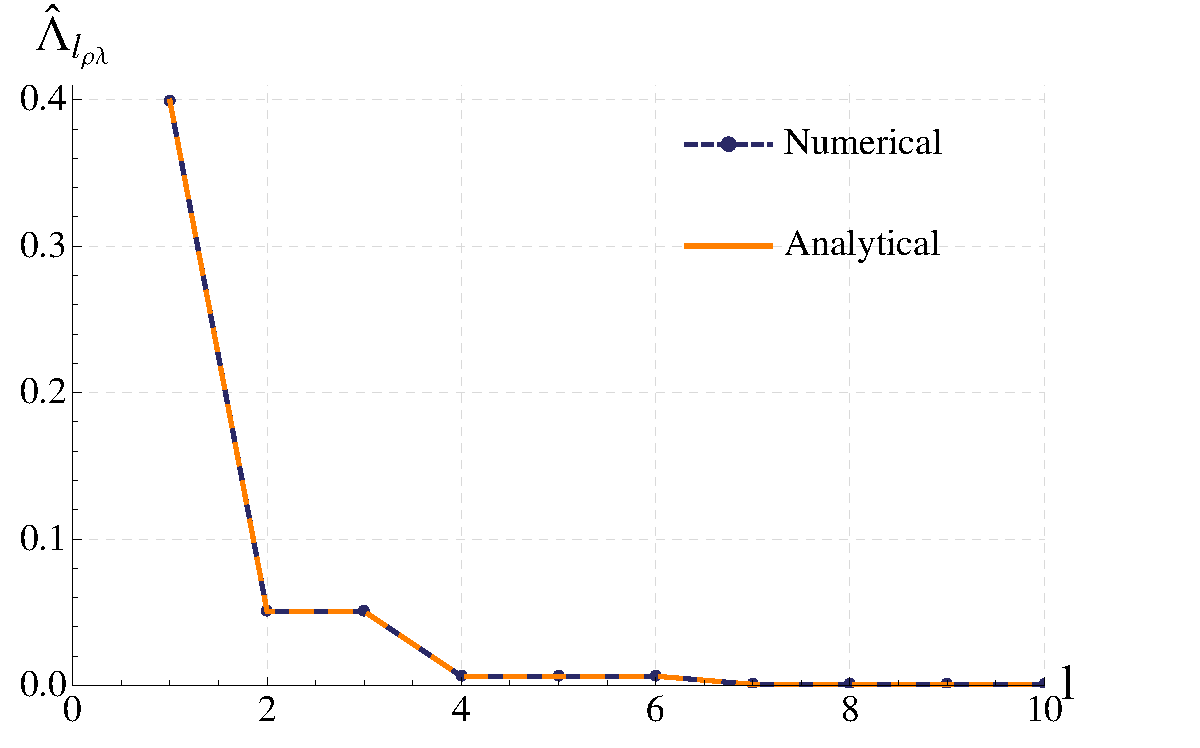
\includegraphics[scale=0.5]{Results/Collagen/Eigensystem/Hypermatrix/Eigenvalues/0.125/lambda_t_ij_L5_m20.pdf}
\caption{Eigenvalues calculated numerically from the transfer hyper-matrix plotted with the analytical eigenvalues calculated by combining $\hat{\lambda}_{l_\rho}$ and $\hat{\lambda}_{l_\lambda}$. The excellent agreement between the numerical and analytical results suggests that we are able to generate the eigenfunctions of the hyper-matrix from the analytical eigenfunctions $\hat{\psi}_{l_\rho}$ and $\hat{\psi}_{l_\lambda}$. These eigenvalues are calculated with $\Delta=0.125$, where $L=5$ and $m=20$.}
\label{fig:collagen_eval_nva}
\end{figure}

%\begin{figure}[htp]
%\centering \includegraphics[scale=0.5]{Results/Collagen/Eigensystem/Hypermatrix/%Eigenvalues/0.125/3D_lambda_ij_L5_m20.pdf}
%\caption{Add something...}
%\label{fig:collagen_eval_3D}
%\end{figure}

%%% Hyper-eigenvector%%%
\begin{figure}[H]
\centering
\begin{tabular}{cc}
\subfloat[]{\label{fig:n_hyp_evec_1}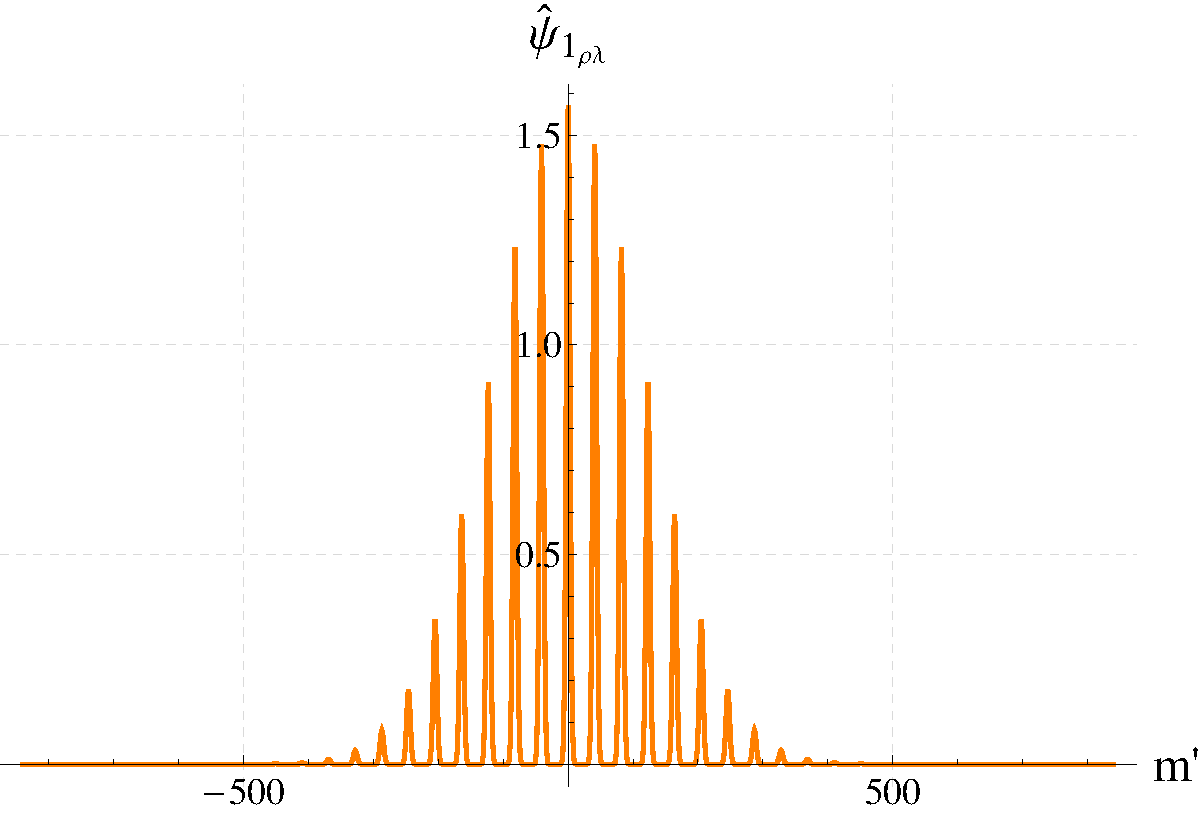
\includegraphics[scale=0.325]{Results/Collagen/Eigensystem/Hypermatrix/Eigenvectors/0.125/N_psi_1_L5_m20_k1.pdf}} &
\subfloat[]{\label{fig:n_hyp_evec_2}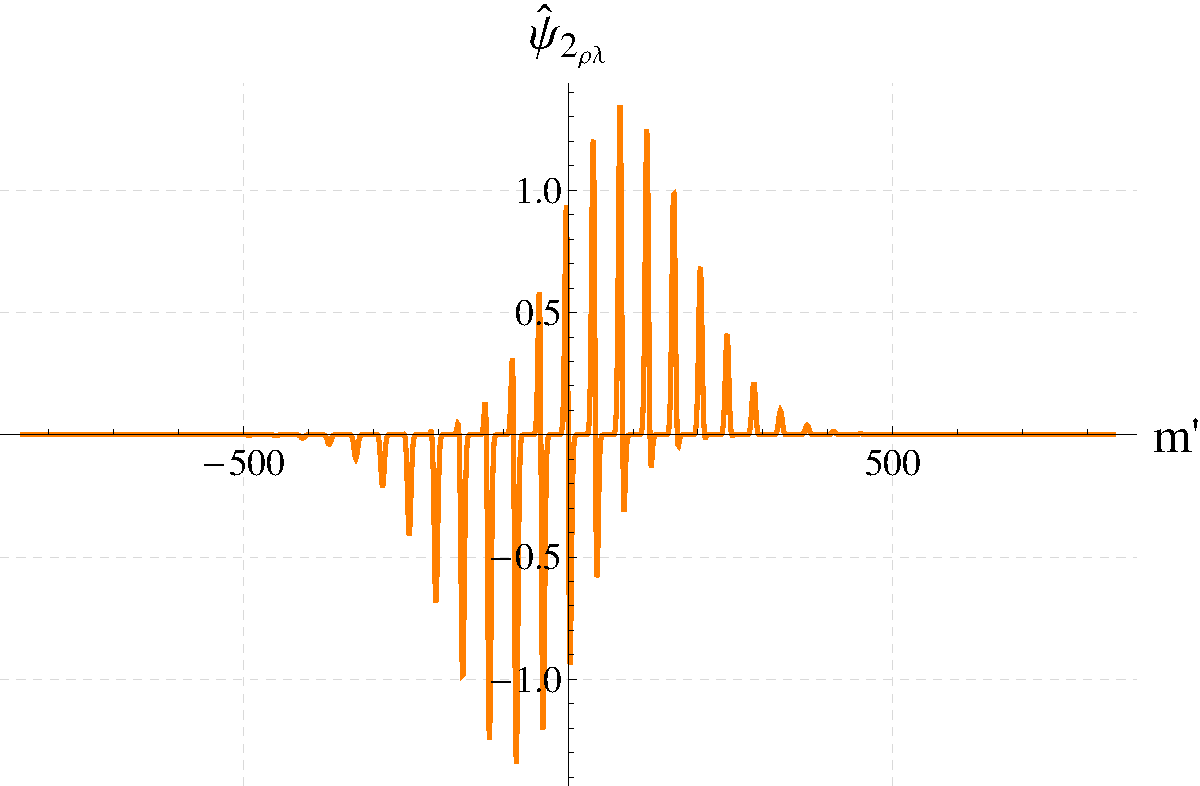
\includegraphics[scale=0.325]{Results/Collagen/Eigensystem/Hypermatrix/Eigenvectors/0.125/N_psi_2_L5_m20_k1.pdf}} \\
\subfloat[]{\label{fig:n_hyp_evec_3}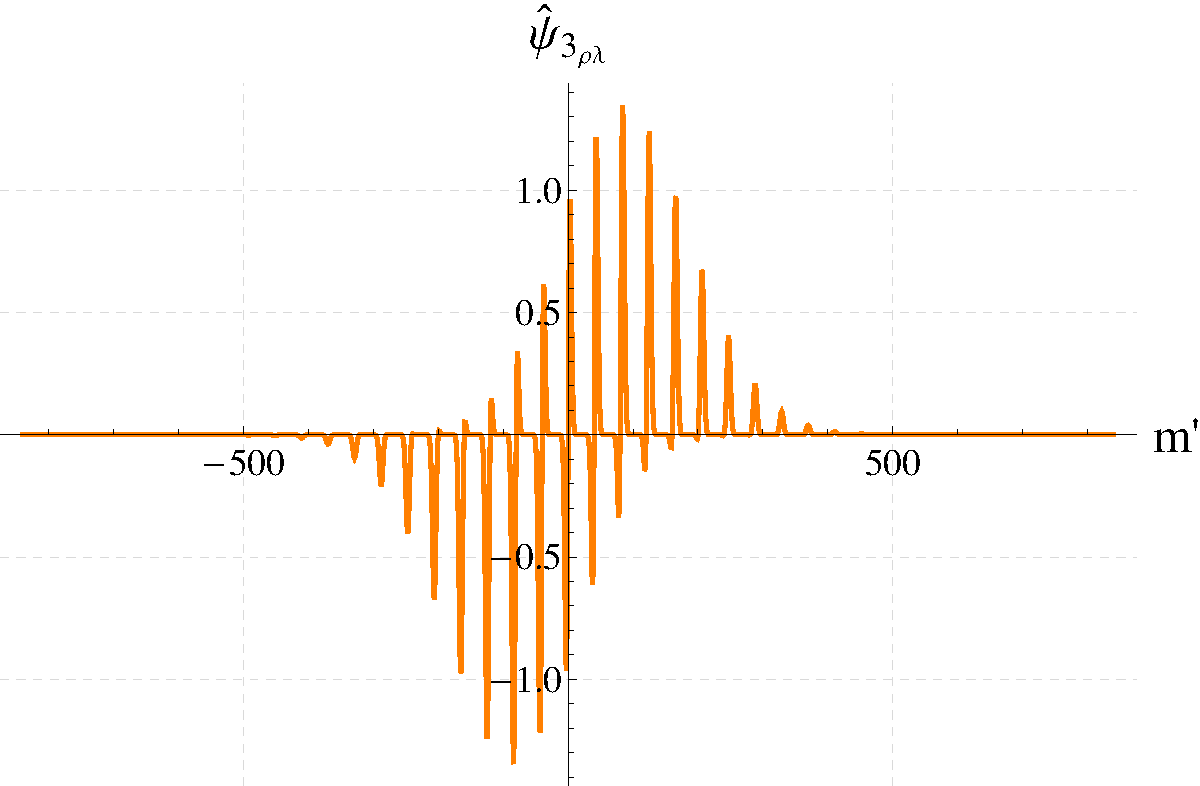
\includegraphics[scale=0.325]{Results/Collagen/Eigensystem/Hypermatrix/Eigenvectors/0.125/N_psi_3_L5_m20_k1.pdf}} &
\subfloat[]{\label{fig:n_hyp_evec_4}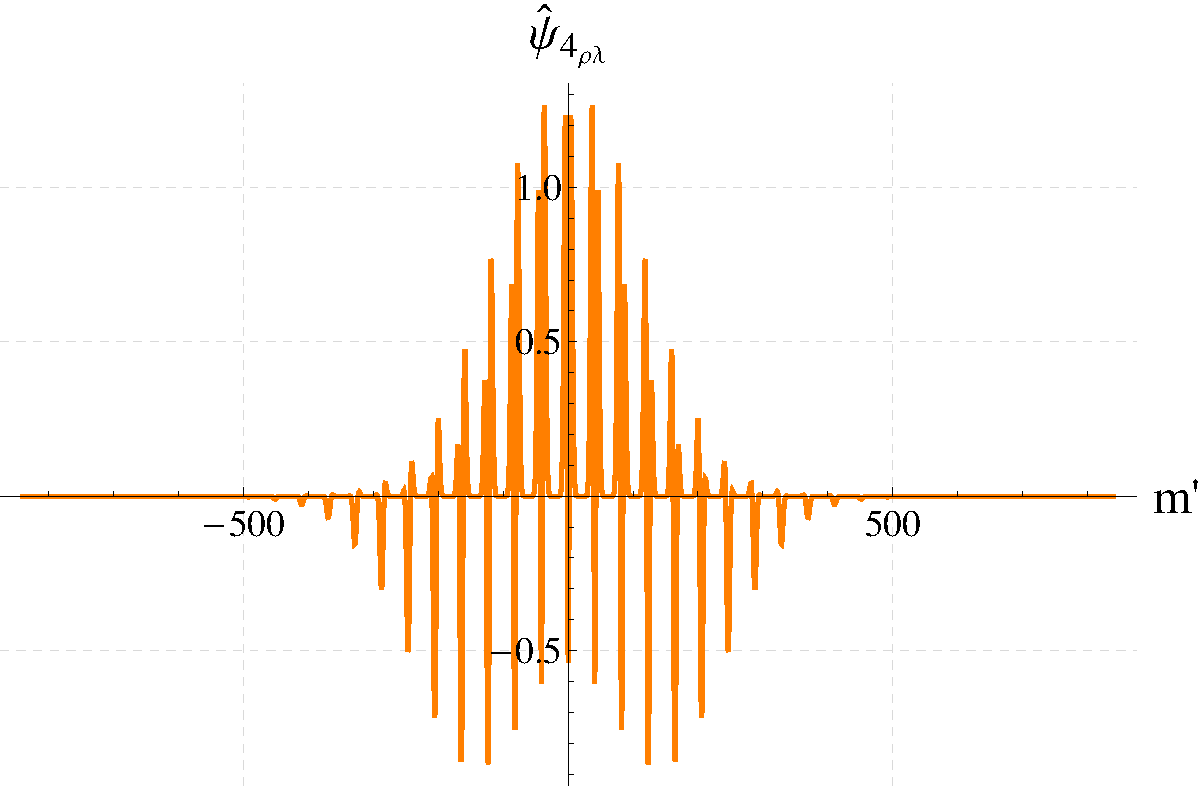
\includegraphics[scale=0.325]{Results/Collagen/Eigensystem/Hypermatrix/Eigenvectors/0.125/N_psi_4_L5_m20_k1.pdf}} \\
\end{tabular}
\caption{A plot of the first four eigenfunctions of the transfer hypermatrix. The hypermatrix was converted to a normal $N\times N$ matrix before the numerical calculation. These eigenfunctions are calculated with $N=(2m+1)^2$ and $\Delta=0.125$, where $L=5$ and $m=20$.}
\label{fig:n_hyp_evec} 
\begin{tabular}{cc}
\subfloat[$\hat{\psi}_{1_{\rho}}\hat{\psi}_{1_{\lambda}}$]{\label{fig:nVa_hyp_evec_1}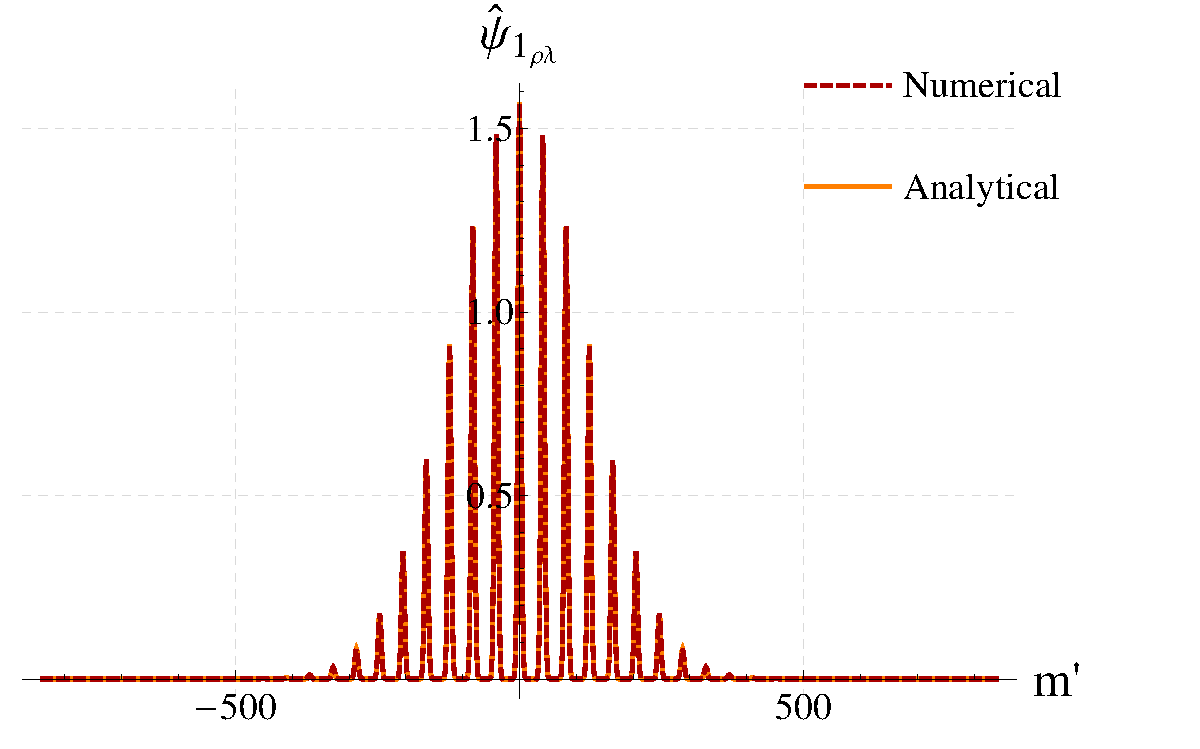
\includegraphics[scale=0.325]{Results/Collagen/Eigensystem/Hypermatrix/Eigenvectors/0.125/NA_psi_1_L5_m20_k1.pdf}} &
\subfloat[$\hat{\psi}_{1_{\rho}}\hat{\psi}_{2_{\lambda}}$]{\label{fig:nVa_hyp_evec_2}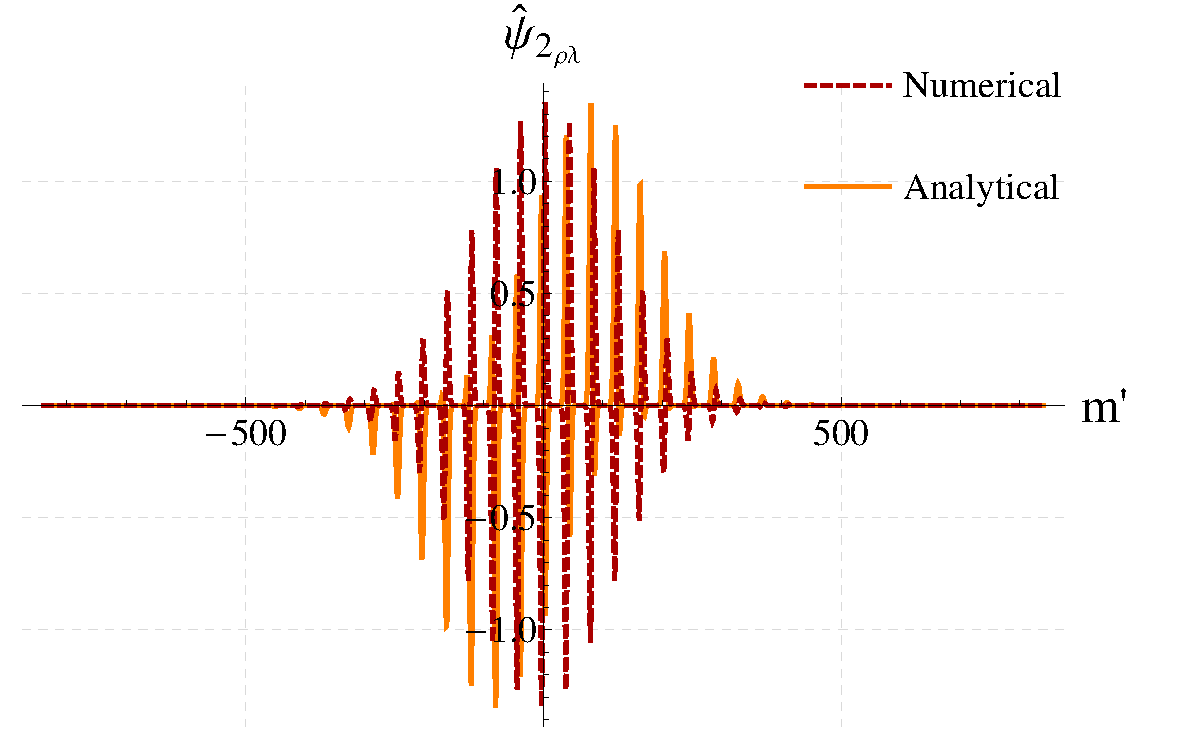
\includegraphics[scale=0.325]{Results/Collagen/Eigensystem/Hypermatrix/Eigenvectors/0.125/NA_psi_2_L5_m20_k1.pdf}} \\
\subfloat[$\hat{\psi}_{2_{\rho}}\hat{\psi}_{1_{\lambda}}$]{\label{fig:nVa_hyp_evec_3}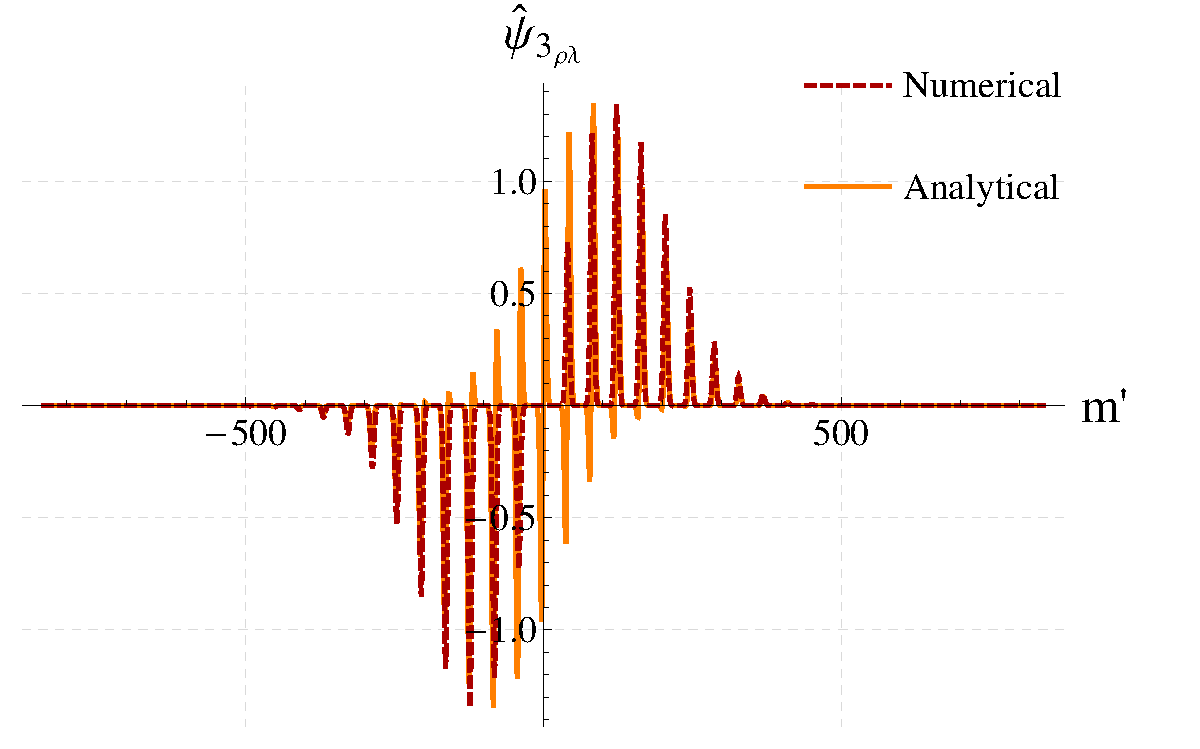
\includegraphics[scale=0.325]{Results/Collagen/Eigensystem/Hypermatrix/Eigenvectors/0.125/NA_psi_3_L5_m20_k1.pdf}} &
\subfloat[$\hat{\psi}_{2_{\rho}}\hat{\psi}_{2_{\lambda}}$]{\label{fig:nVa_hyp_evec_4}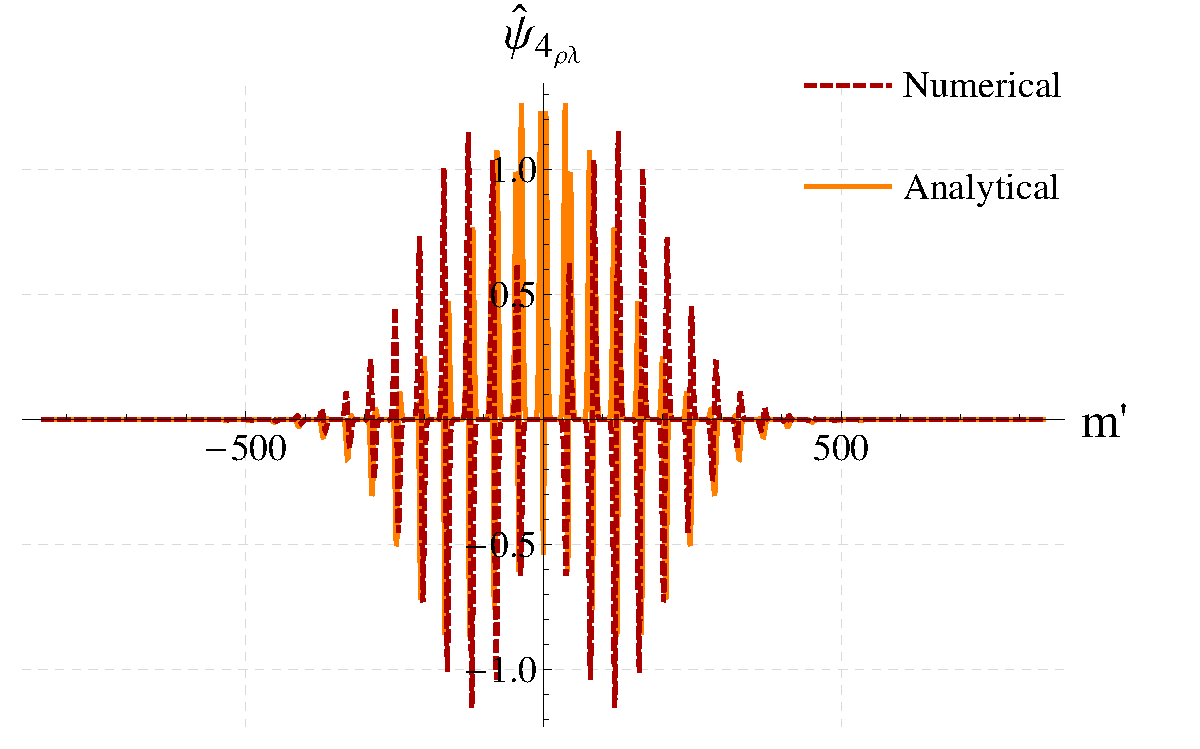
\includegraphics[scale=0.325]{Results/Collagen/Eigensystem/Hypermatrix/Eigenvectors/0.125/NA_psi_4_L5_m20_k1.pdf}} \\
\end{tabular}
\caption{In addition to results shown in \figref{n_hyp_evec} we plot eigenfunctions that were reproduced by the analytical eigenfunctions $\hat{\psi}_{l_\rho}$ and $\hat{\psi}_{l_\lambda}$. }
\label{fig:nVa_hyp_evec} 
\end{figure}

%%% Hyper-eigenvector 3D%%%
%\begin{figure}[H]
%\centering
%\begin{tabular}{cc}
%\subfloat[$\hat{\psi}_{1_{\rho\lambda}}(\rho,\lambda)$]{\label{fig:3D_n_hyp_evec_1}\includegraphics%[scale=0.325]{Results/Collagen/Eigensystem/Hypermatrix/Eigenvectors/0.125/3D_N_psi_1_L5_m20_k1.pdf}} &
%\subfloat[$\hat{\psi}_{2_{\rho\lambda}}(\rho,\lambda)$]{\label{fig:3D_n_hyp_evec_2}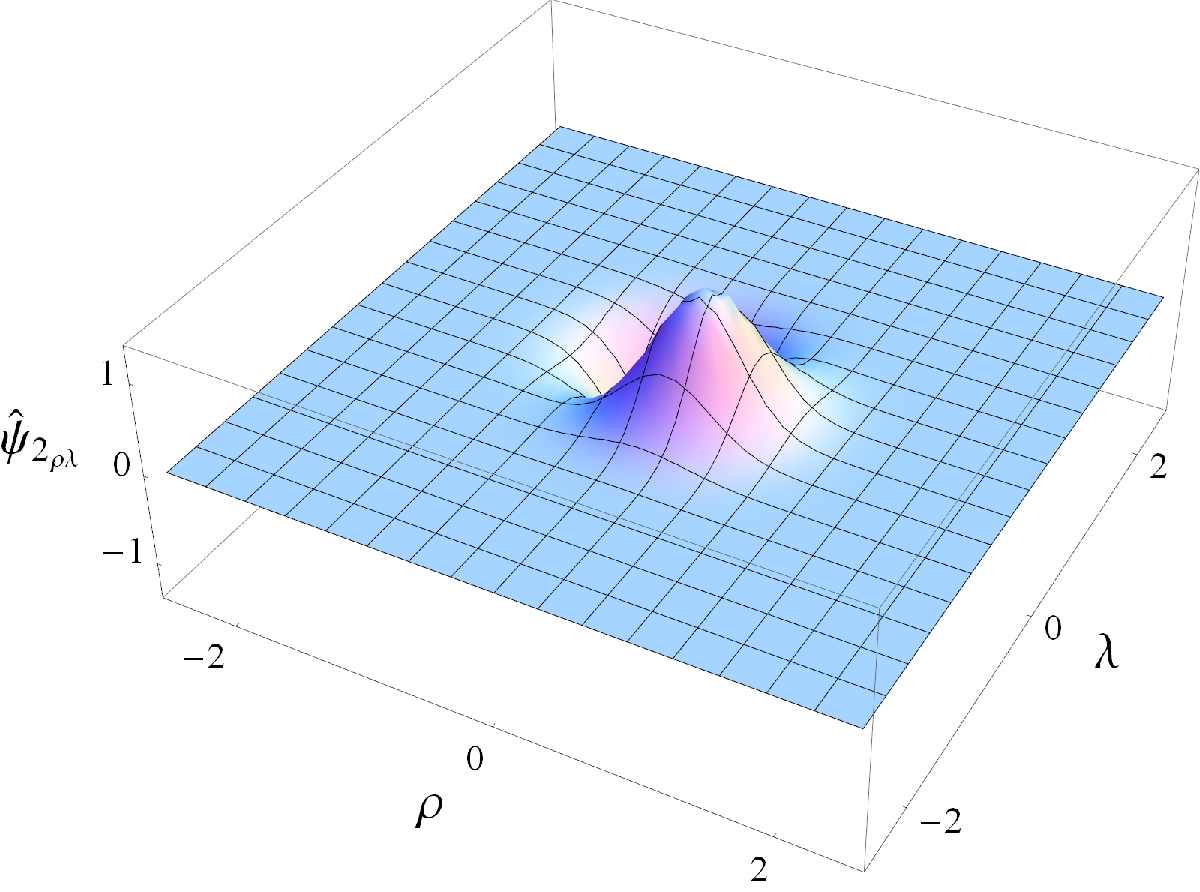
\includegraphics[scale=0.325]{Results/Collagen/Eigensystem/Hypermatrix/Eigenvectors/0.125/3D_N_psi_2_L5_m20_k1.pdf}} \\
%\subfloat[$\hat{\psi}_{3_{\rho\lambda}}(\rho,\lambda)$]{\label{fig:3D_n_hyp_evec_3}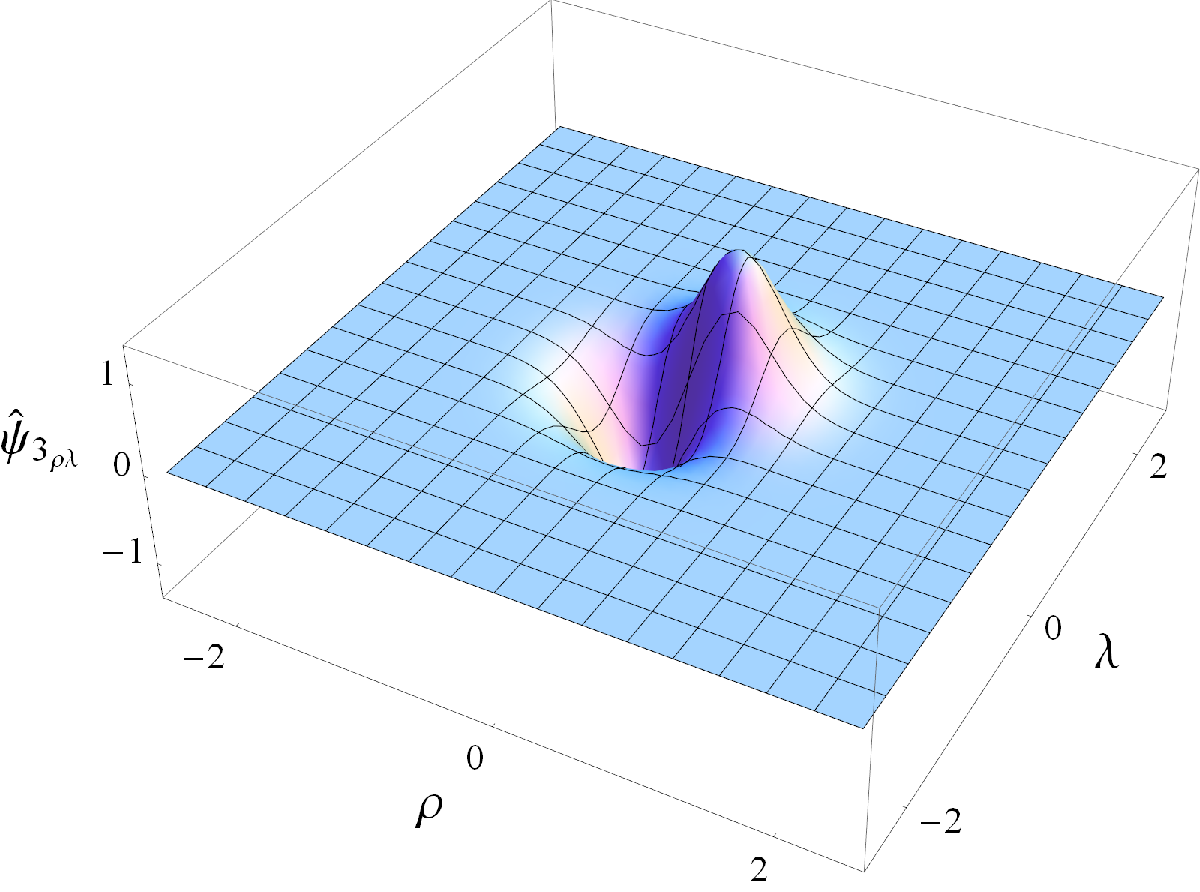
\includegraphics[scale=0.325]{Results/Collagen/Eigensystem/Hypermatrix/Eigenvectors/0.125/3D_N_psi_3_L5_m20_k1.pdf}} &
%\subfloat[$\hat{\psi}_{4_{\rho\lambda}}(\rho,\lambda)$]{\label{fig:3D_n_hyp_evec_4}\includegraphics[scale=0.325]{Results/Collagen/Eigensystem/Hypermatrix/Eigenvectors/0.125/3D_N_psi_4_L5_m20_k1.pdf}} \\
%\end{tabular}
%\caption{3D plots of the first four hypermatrix eigenfunctions when converted back into two variable eigenfunctions. These eigenfunctions are calculated with $\Delta=0.125$, where $L=5$ and $m=20$.}
%\label{fig:3D_n_hyp_evec} 
%\begin{tabular}{cc}
%\subfloat[$\hat{\psi}_{1}(\rho)\hat{\psi}_{1}(\lambda)$]{\label{fig:3D_a_hyp_evec_1}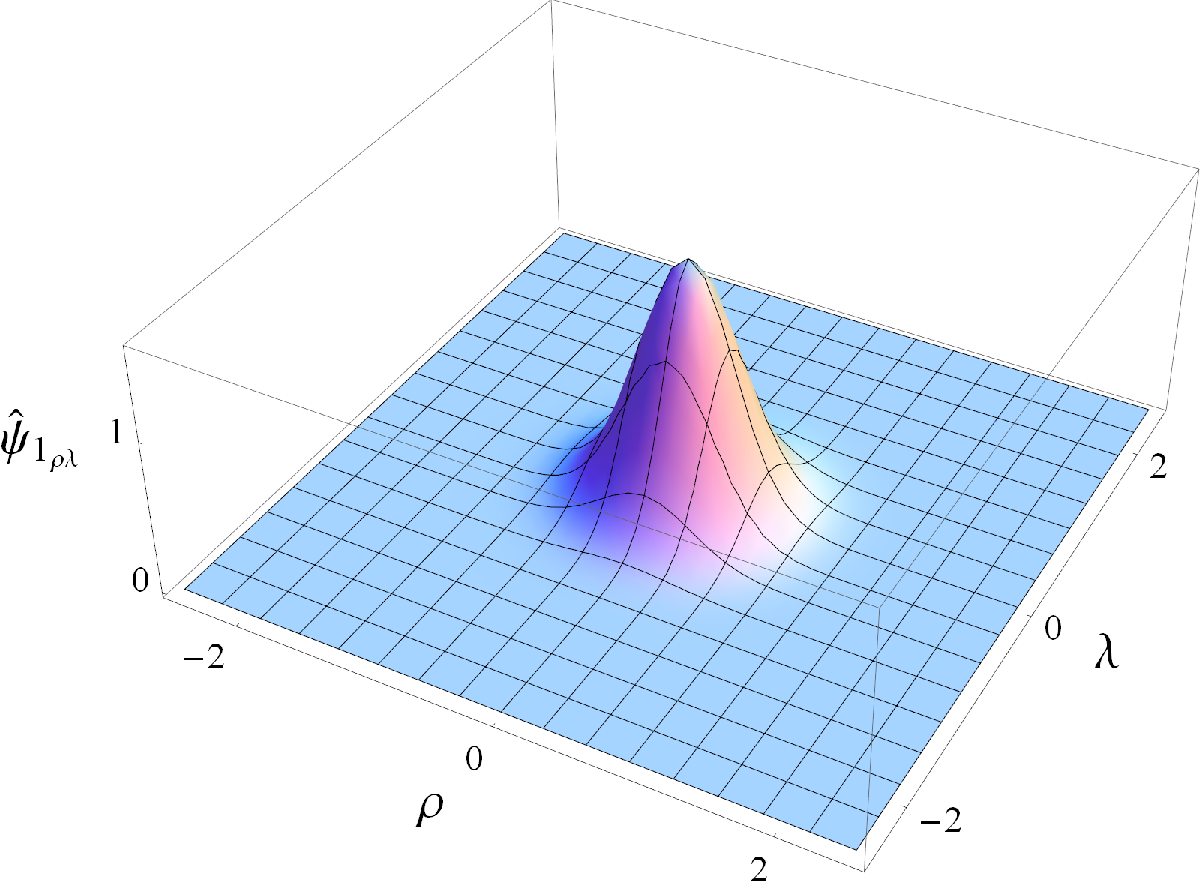
\includegraphics[scale=0.325]{Results/Collagen/Eigensystem/Hypermatrix/Eigenvectors/0.125/3D_A_psi_00_L5_m20_k1.pdf}} &
%\subfloat[$\hat{\psi}_{1}(\rho)\hat{\psi}_{2}(\lambda)$]{\label{fig:3D_a_hyp_evec_2}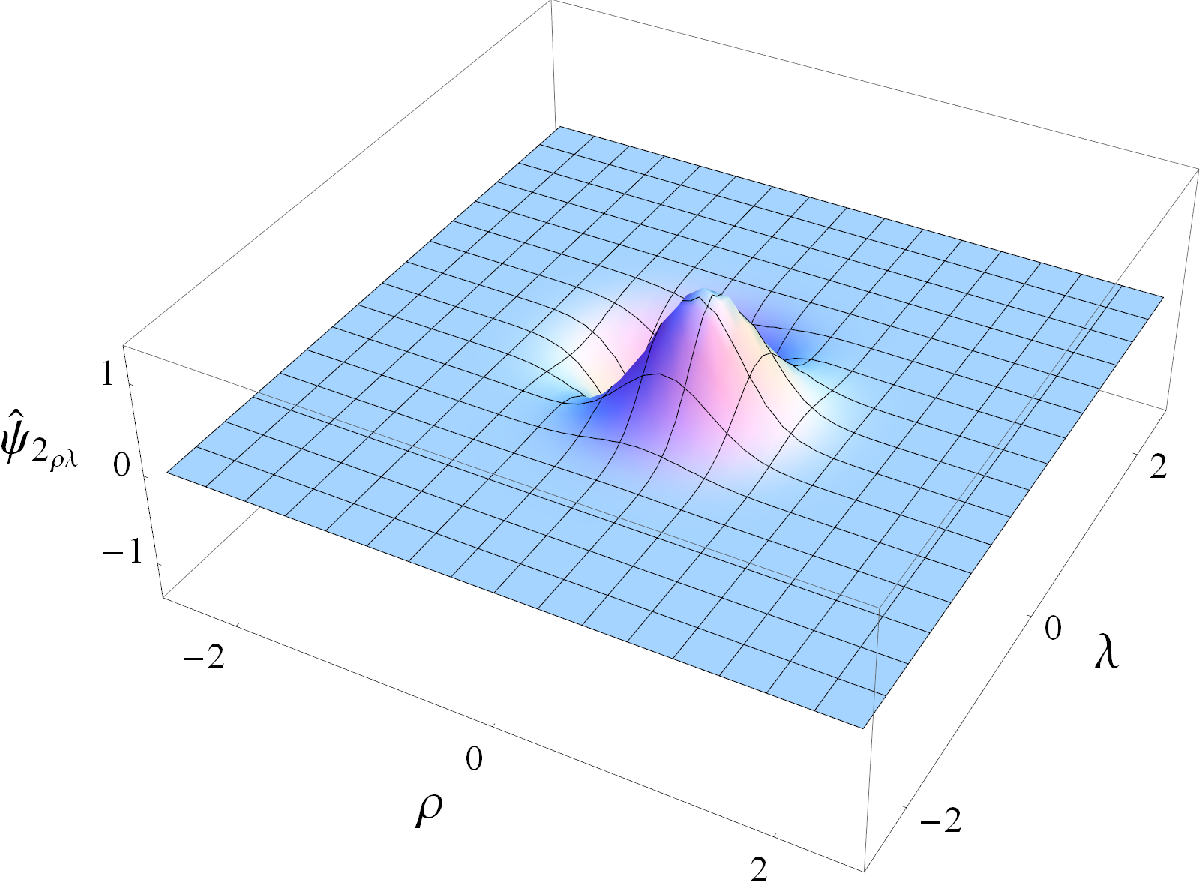
\includegraphics[scale=0.325]{Results/Collagen/Eigensystem/Hypermatrix/Eigenvectors/0.125/3D_A_psi_10_L5_m20_k1.pdf}} \\
%\subfloat[$\hat{\psi}_{2}(\rho)\hat{\psi}_{1}(\lambda)$]{\label{fig:3D_a_hyp_evec_3}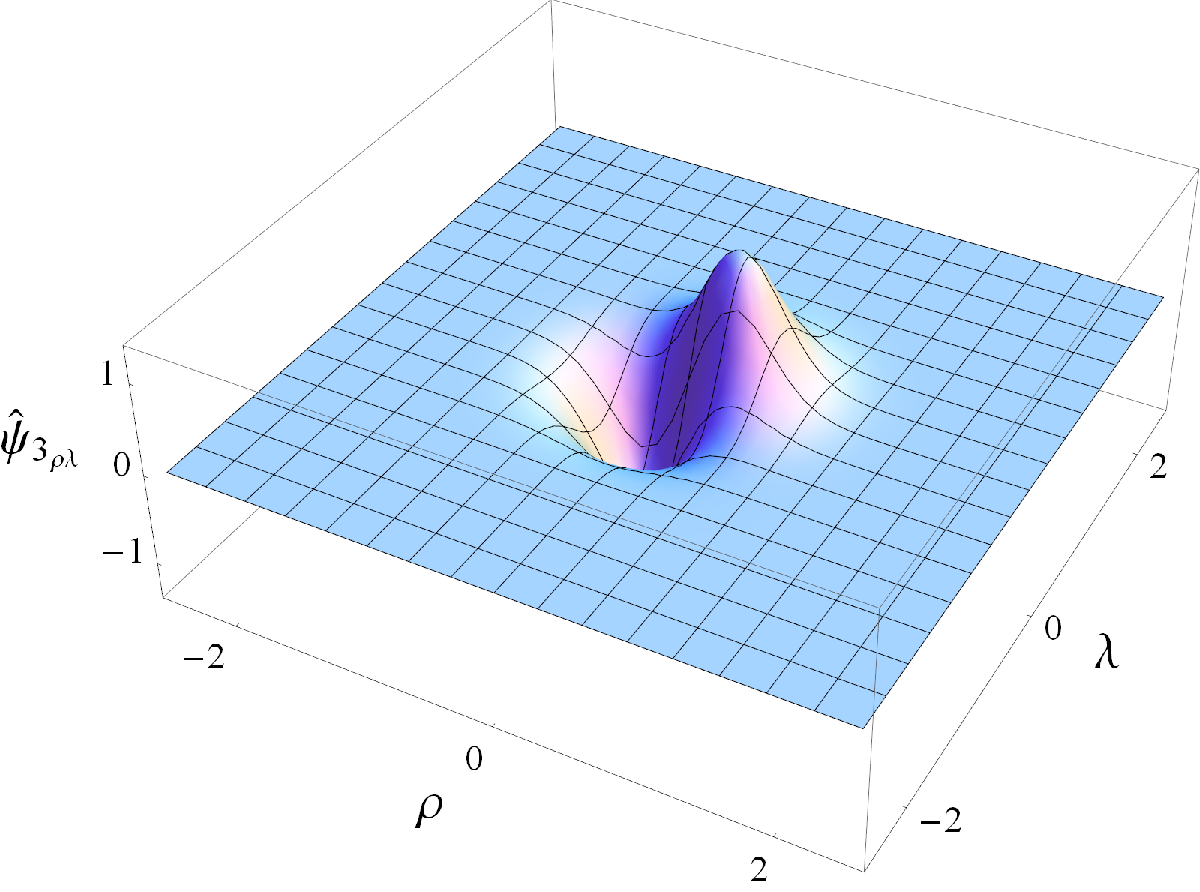
\includegraphics[scale=0.325]{Results/Collagen/Eigensystem/Hypermatrix/Eigenvectors/0.125/3D_A_psi_01_L5_m20_k1.pdf}} %&
%\subfloat[$\hat{\psi}_{2}(\rho)\hat{\psi}_{2}(\lambda)$]{\label{fig:3D_a_hyp_evec_4}\includegraphics[scale=0.325]{Results/Collagen/Eigensystem/Hypermatrix/Eigenvectors/0.125/3D_A_psi_11_L5_m20_k1.pdf}} \\
%\end{tabular}
%\caption{3D plots created from the analytical eigenfunctions $\hat{\psi}_{l_\rho}$ and $\hat{\psi}_{l_\lambda}$ that demonstrates the reproduction of the hypermatrix eigenfunctions. In order match the second and third eigenfunctions we had to apply a rotation of $\pi/4$ about the z-axis.}
%\label{fig:3D_a_hyp_evec} 
%\end{figure}

%%% Hyper-eigenvector 3D%%%
\begin{figure}[H]
\centering
\begin{tabular}{cc}
\subfloat[$\hat{\psi}_{1_{\rho\lambda}}(\rho,\lambda)$]{\label{fig:3D_n_hyp_evec_1}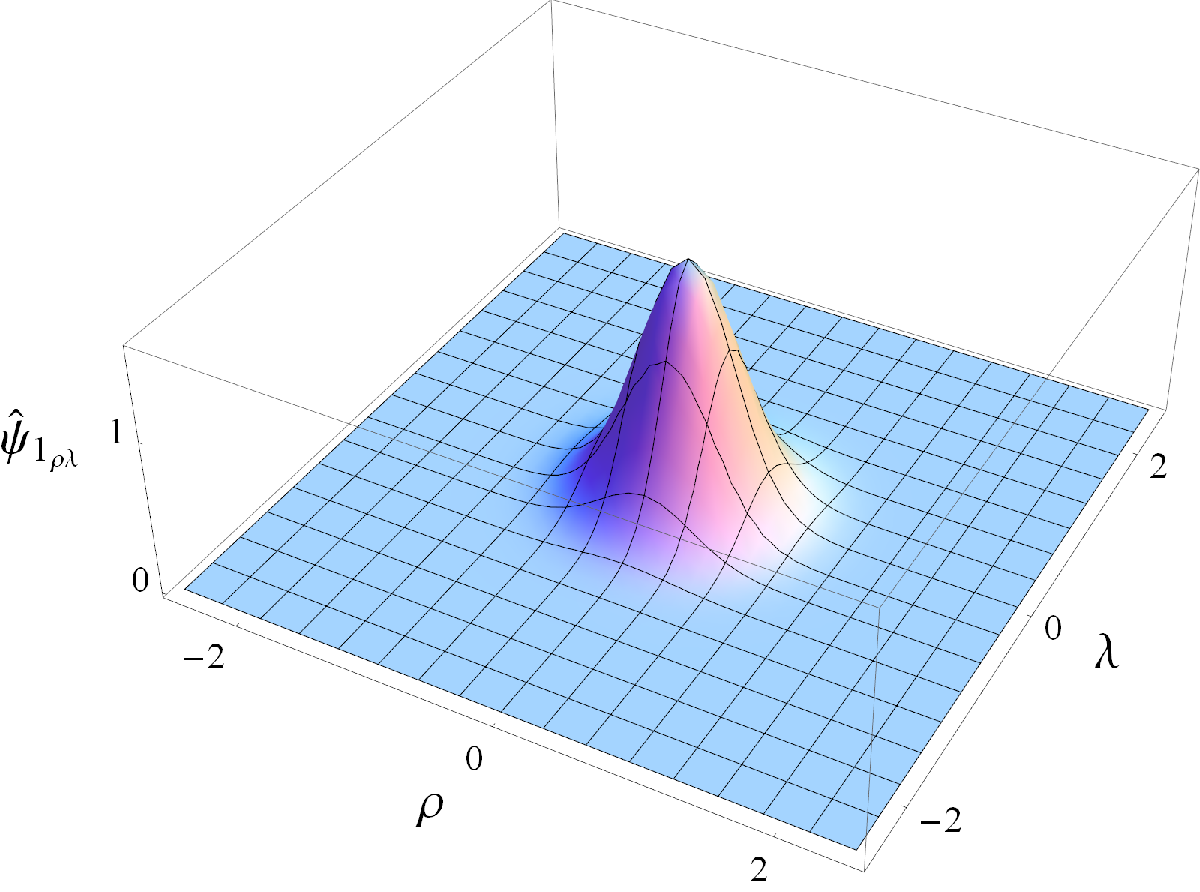
\includegraphics[scale=0.45]{Results/Collagen/Eigensystem/Hypermatrix/Eigenvectors/0.125/3D_N_psi_1_L5_m20_k1.pdf}} \\
\subfloat[$\hat{\psi}_{2_{\rho\lambda}}(\rho,\lambda)$]{\label{fig:3D_n_hyp_evec_2}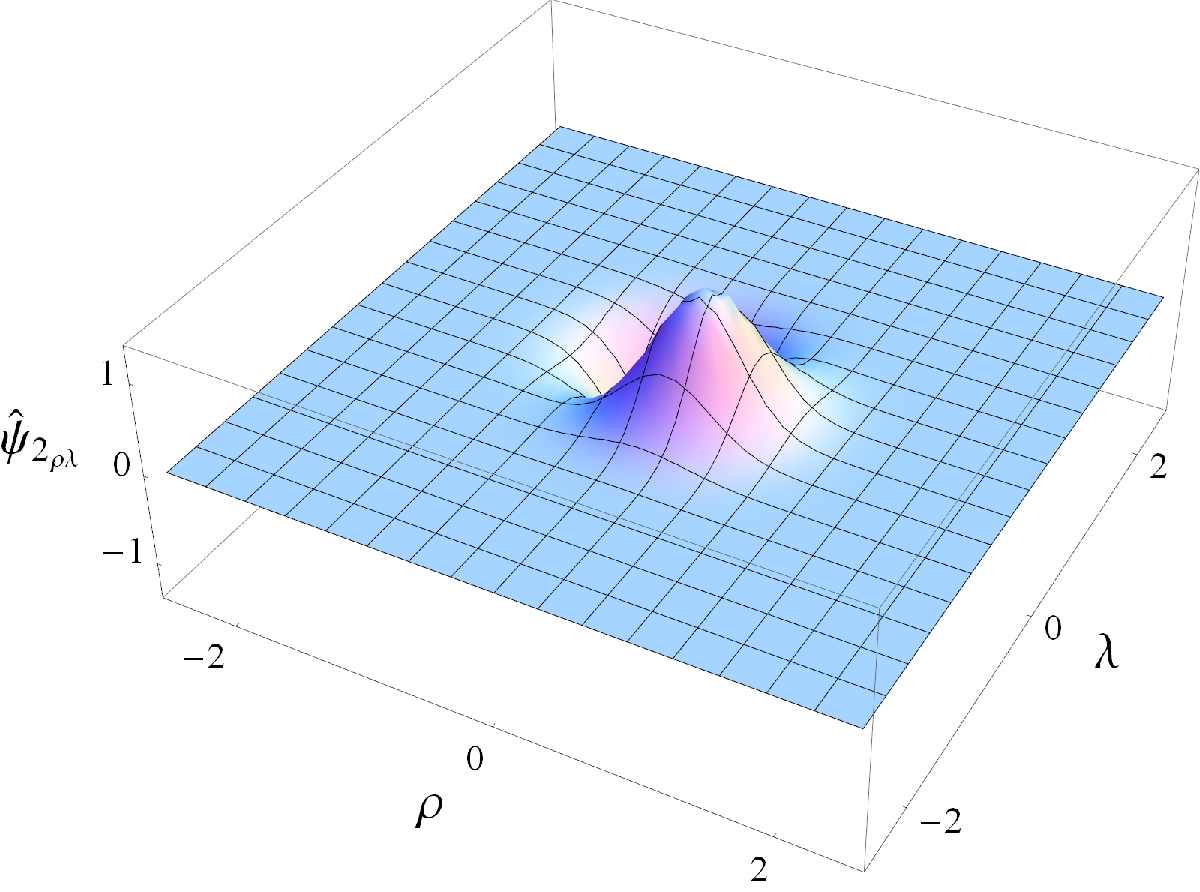
\includegraphics[scale=0.45]{Results/Collagen/Eigensystem/Hypermatrix/Eigenvectors/0.125/3D_N_psi_2_L5_m20_k1.pdf}} \\
\subfloat[$\hat{\psi}_{3_{\rho\lambda}}(\rho,\lambda)$]{\label{fig:3D_n_hyp_evec_3}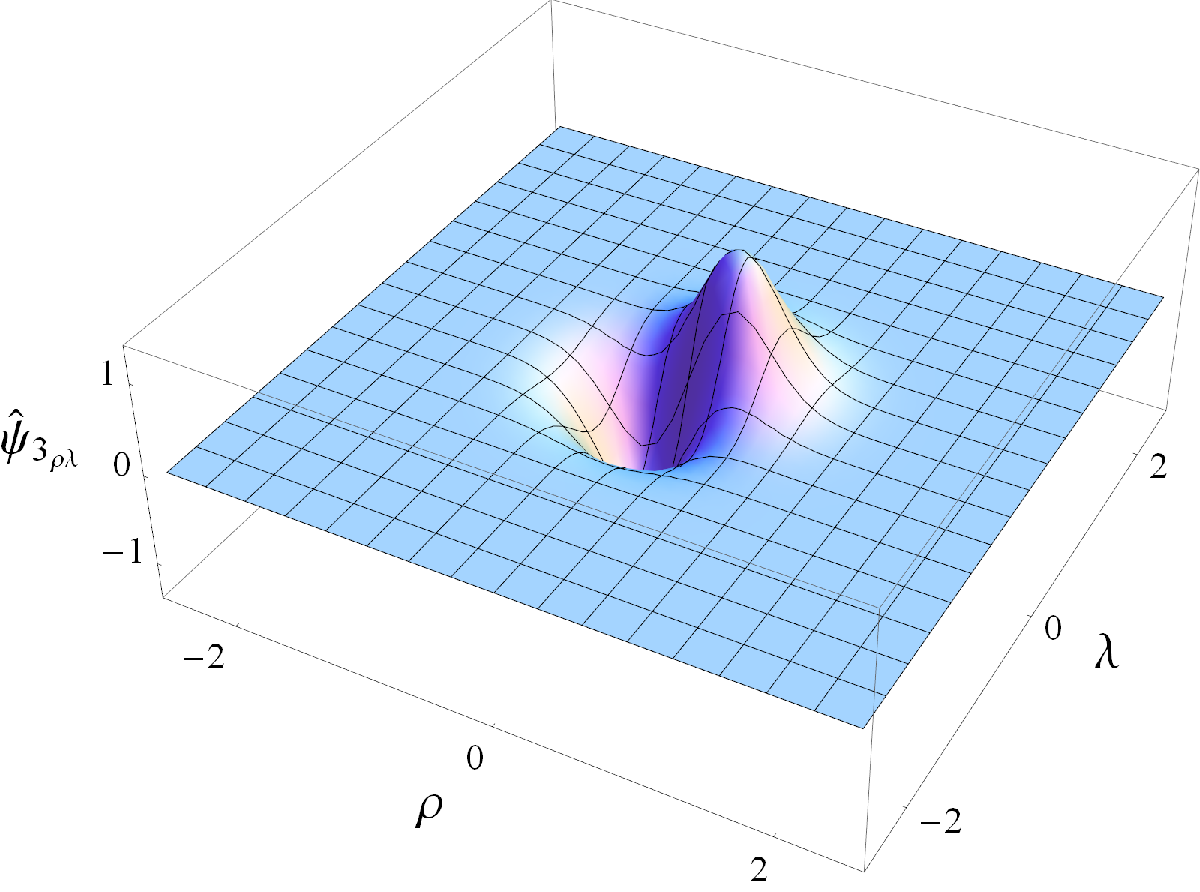
\includegraphics[scale=0.45]{Results/Collagen/Eigensystem/Hypermatrix/Eigenvectors/0.125/3D_N_psi_3_L5_m20_k1.pdf}}
\end{tabular}
\caption{2D plots of the first 3 hypermatrix eigenfunctions when converted back into two variable eigenfunctions.These eigenfunctions are calculated with $\Delta=0.125$, where $L=5$ and $m=20$.}
\label{fig:3D_n_hyp_evec} 
\end{figure}

\newpage

\begin{figure}[H]
\centering
\begin{tabular}{cc}
\subfloat[$\hat{\psi}_{1_{\rho\lambda}}(\rho,\lambda)=\hat{\psi}_{1}(\rho)\hat{\psi}_{1}(\lambda)$]{\label{fig:3D_a_hyp_evec_1}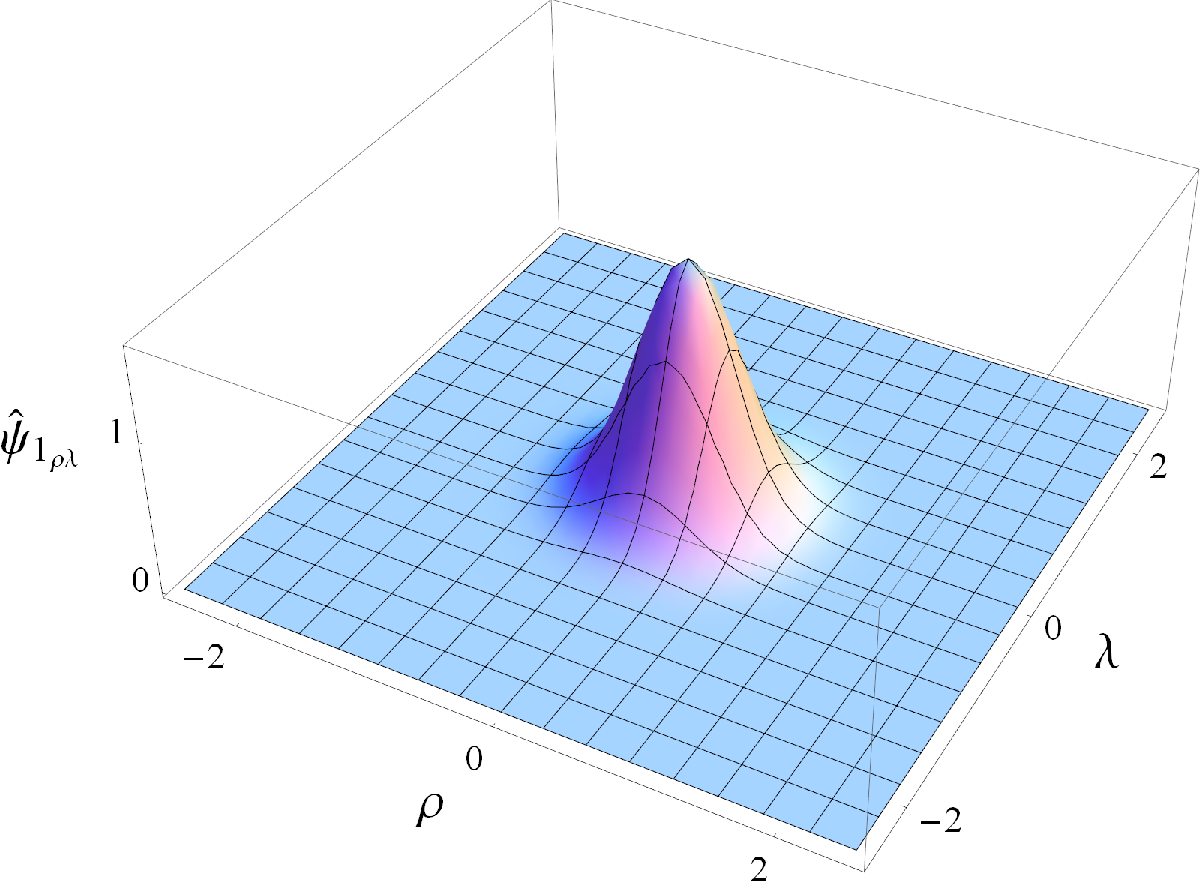
\includegraphics[scale=0.45]{Results/Collagen/Eigensystem/Hypermatrix/Eigenvectors/0.125/3D_A_psi_00_L5_m20_k1.pdf}} \\
\subfloat[$\hat{\psi}_{2_{\rho\lambda}}(\rho,\lambda)=\hat{\psi}_{1}(\rho)\hat{\psi}_{2}(\lambda)$]{\label{fig:3D_a_hyp_evec_2}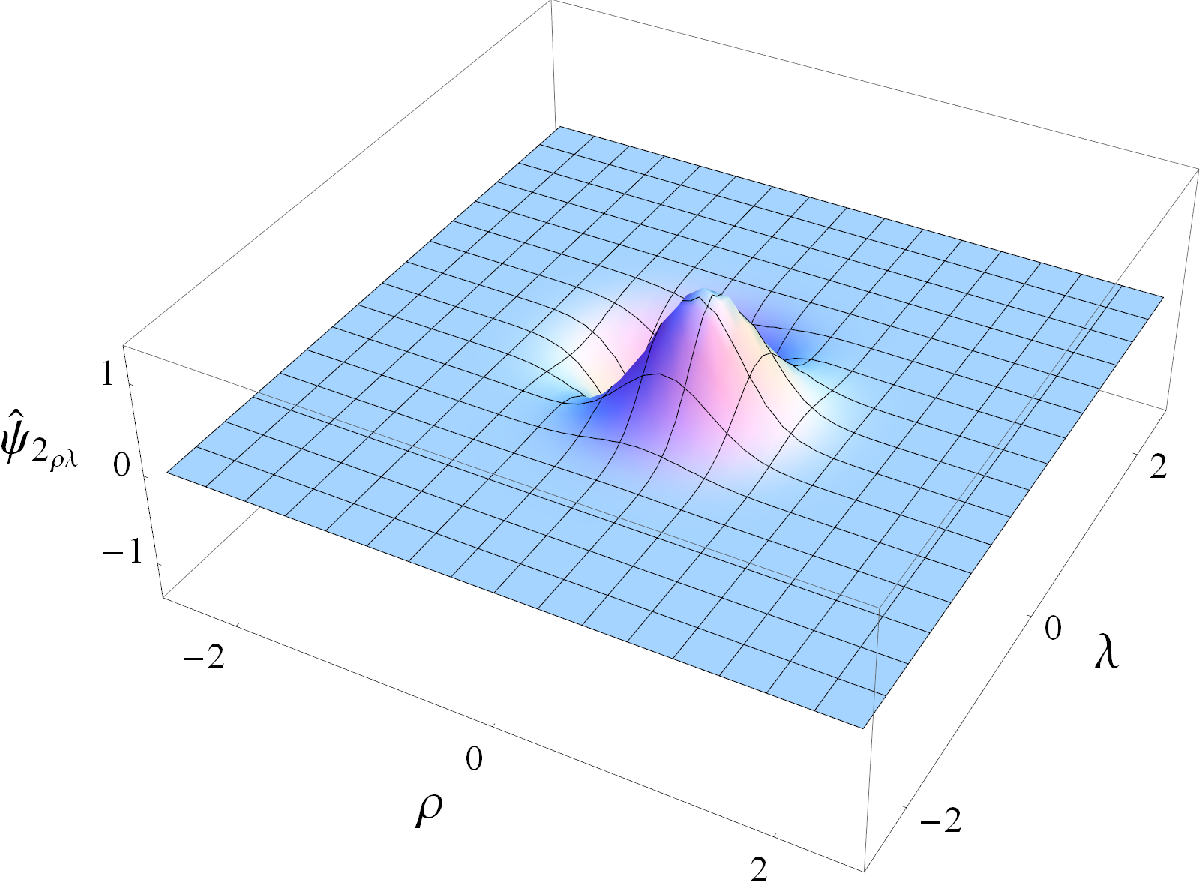
\includegraphics[scale=0.45]{Results/Collagen/Eigensystem/Hypermatrix/Eigenvectors/0.125/3D_A_psi_10_L5_m20_k1.pdf}} \\
\subfloat[$\hat{\psi}_{3_{\rho\lambda}}(\rho,\lambda)=\hat{\psi}_{2}(\rho)\hat{\psi}_{1}(\lambda)$]{\label{fig:3D_a_hyp_evec_3}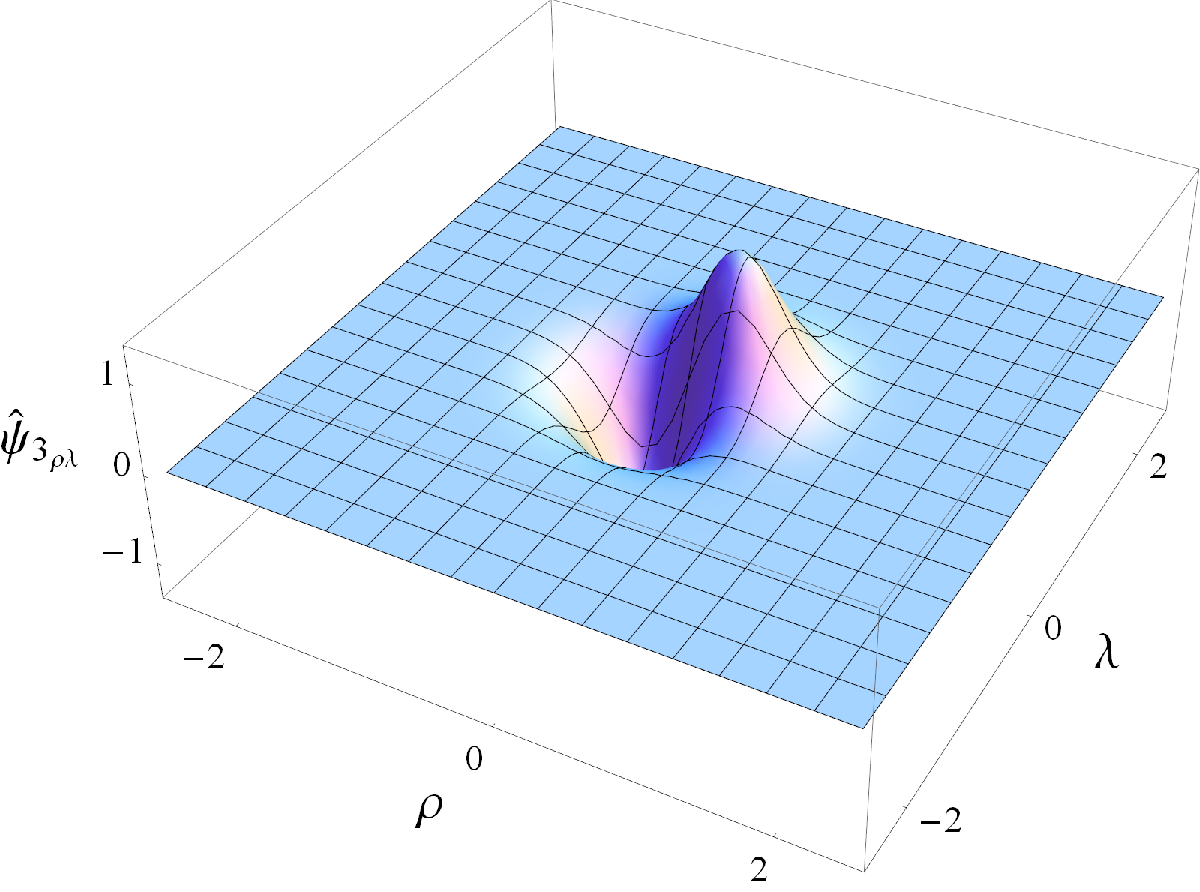
\includegraphics[scale=0.45]{Results/Collagen/Eigensystem/Hypermatrix/Eigenvectors/0.125/3D_A_psi_01_L5_m20_k1.pdf}}
\end{tabular}
\caption{2D plots created from the analytical eigenfunctions $\hat{\psi}_{l_\rho}$ and $\hat{\psi}_{l_\lambda}$ that demonstrates the reproduction of the hypermatrix eigenfunctions. In order to match the second and third eigenfunctions we had to apply a rotation of $\pi/4$ about the $z$-axis.}
\label{fig:3D_a_hyp_evec} 
\end{figure}


\newpage
\section{Results for collagen model calculations}

Our analysis of the simplified collagen structure gives us two descriptions of the collagen model. The first collagen model is for a general potential $V$ representing the residue pairs in the collagen structure that uses the hypermatrix analysis to evaluate the partition function through semi-analytical eigenfunctions. In the second collagen model,  the harmonic collagen model, a harmonic potential was used used early in the analysis of the partition function. This greatly simplified the calculations to express the partition function through the full sets of analytical eigenfunctions that we obtained in DNA for $\eta_{B}=\infty$. In both these models we now go beyond the free energy calculations to describe the force extension behaviour for a given $u$. 

The models use different calculation methods to evaluate the partition function, but by using a harmonic potential for the residue pair we should return similar results for the partition function. The results shown in \figref{nVa_1} compares the two models when we use a harmonic potential in the general collagen model. The excellent agreement between the two results validates the hyper-matrix calculations in the general model. Both collagen models show that for a harmonic potential there is a constant restoring force for an applied extension. The periodicity of the force-extension curves at $u \approx 2.25$ arises from the periodic constraints on $\psi_{l_{R}}$. 

\begin{figure}[H]
\centering
\begin{tabular}{cc}
\subfloat[]{\label{fig:nVa_fe_1}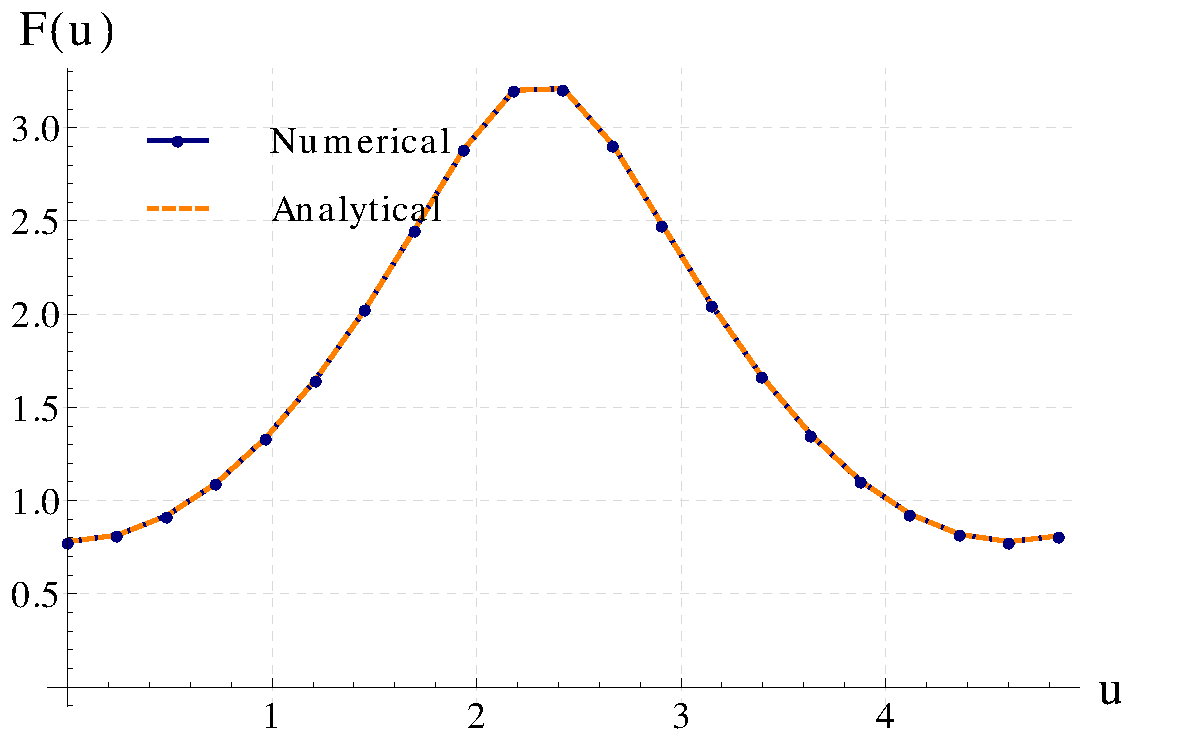
\includegraphics[scale=0.325]{Results/Collagen/nVa/col_f_N5_L8_m16_kappa1_sigma1}} &
\subfloat[]{\label{fig:nVa_force_ext_1}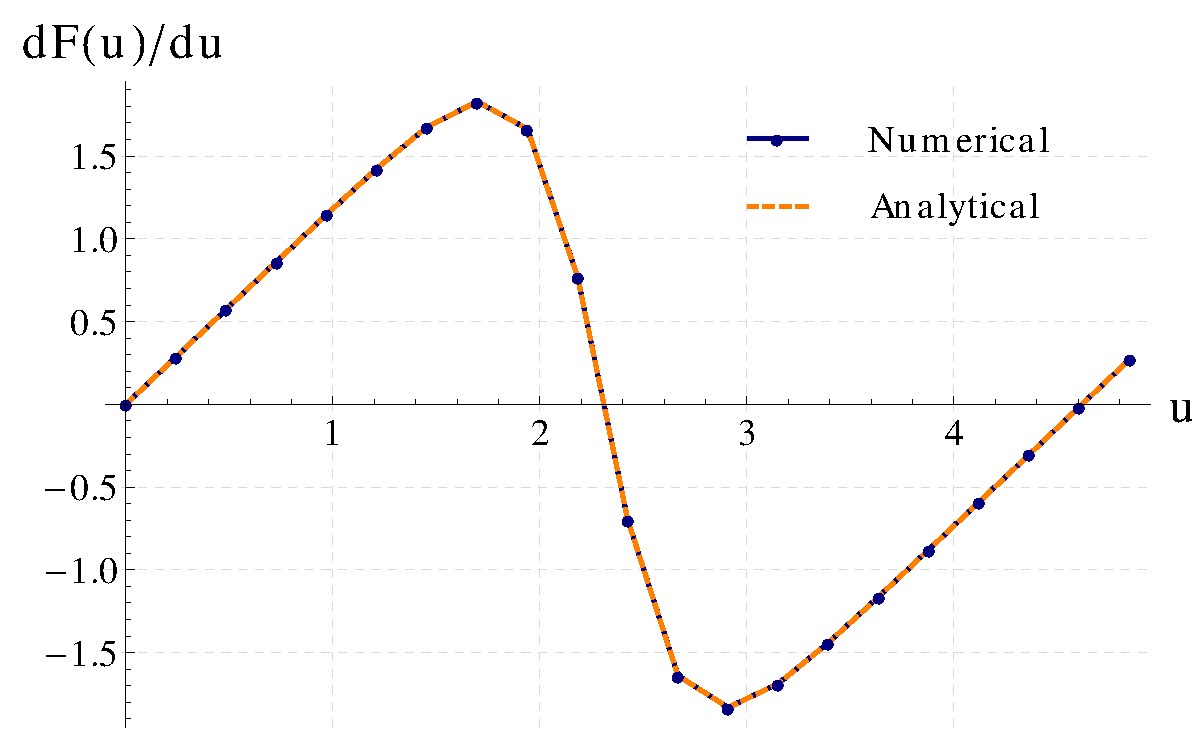
\includegraphics[scale=0.325]{Results/Collagen/nVa/col_df_N5_L8_m16_kappa1_sigma1}} \\
\subfloat[]{\label{fig:nVa_fe_25}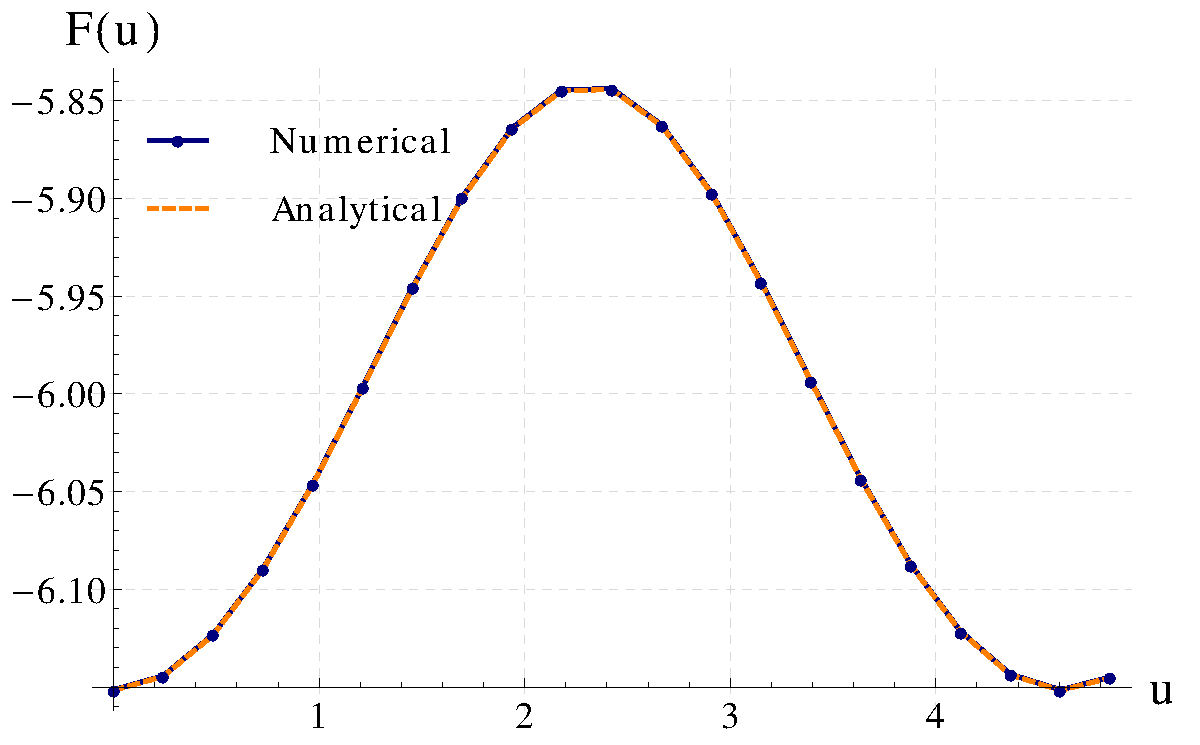
\includegraphics[scale=0.325]{Results/Collagen/nVa/col_f_N5_L8_m16_kappa25_sigma1}} &
\subfloat[]{\label{fig:nVa_force_ext_25}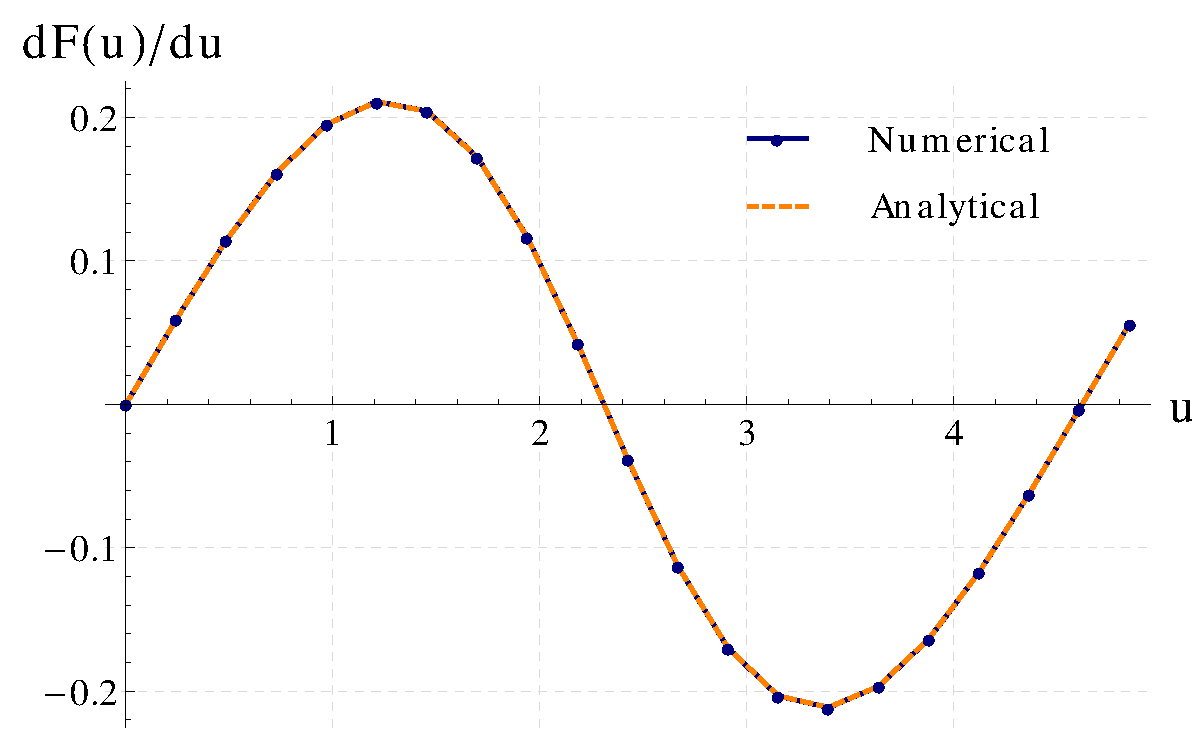
\includegraphics[scale=0.325]{Results/Collagen/nVa/col_df_N5_L8_m16_kappa25_sigma1}} 
\end{tabular}
\caption{A comparison of the results generated by the numerical and semi-analytical calculations of the free energy for harmonic collagen, and its differential with respect to $u$. The excellent agreement between the two results is found for different $\kappa/\kappa'$ ratios as shown in Figs.~\ref{fig:nVa_fe_1}-\ref{fig:nVa_force_ext_1} for $\kappa/\kappa'=1$, and Figs.~\ref{fig:nVa_fe_25}-\ref{fig:nVa_force_ext_25} for $\kappa/\kappa'=25$. These calculations were run with $L=8$, and $m=16$. }
\label{fig:nVa_1} 
\end{figure}

Using the general collagen model we explore different force-extension curves by applying different potentials for the residue pair interactions. In \figref{collagen_pe} we demonstrate a comparison of two such potentials with a pure harmonic interaction that has a constant stiffness of $\kappa'_{ref}=1 \text{ eV/\AA}^{2}$. They are described as follows:

\begin{enumerate}
\item \textbf{Soft-Hard} - is a two step anharmonic potential described by two different stiffness constants in the residue pair potential where there is a transition from $\kappa'_{soft} \to \kappa'_{hard}$ as the extension increases above a threshold. The term "Soft" indicates a potential with a low stiffness constant $\kappa'_{soft}=0.0625 \text{ eV/\AA}^{2}$ whereas "Hard" refers to a high stiffness constant $\kappa'_{hard}=8 \text{ eV/\AA}^{2}$, hence $\kappa'_{soft} < \kappa'_{ref} < \kappa'_{hard}$. 

\begin{comment}Compared with the free energy curve of the harmonic potential, the Soft-to-Hard potential has a much lower free energy curve resulting in a lower restoring force that steadily increases with $u$ shown in \figref{collagen_fe}. The strengthening of the restoring force observed in \figref{collagen_dfe} is a result of base-pairs reaching their limit in $\eta$ of the Soft region, and experiencing the transition of the stiffness constant into the Harder region. More energy is required to extend the structure resulting in a larger restoring force.
\end{comment}

\item \textbf{Hard-Soft} - is an opposite description of the Soft-Hard potential. It is a two step anharmonic potential where the stiffness constant in the residue pair potential makes a transition from $\kappa'_{hard} \to \kappa'_{soft}$ as the extension increases above a threshold. In this potential $\kappa'_{soft}=0.0625 \text{ eV/\AA}^{2}$ and $\kappa'_{hard}=16 \text{ eV/\AA}^{2}$.

\begin{comment}
In \figref{collagen_fe} we see that free energy curve in comparison with the harmonic potential is significantly higher, and steadily increasing with an applied extension. However, it is the rate at which the free energy increases (the restoring force) that represents the effect of the Hard-Soft potential. Shown in \figref{collagen_dfe}, we observe the effect of the Hard stiffness constant resulting in a larger restoring force than the harmonic potential, once the residue pair separation reaches the transition point at $\eta=0.5$ the restoring force reduces proportionally to the Soft stiffness constant.
\end{comment}
\end{enumerate}

The free energy calculations, and force-extension curves for these residue pair potentials are shown in \figref{collagen_fe} and \figref{collagen_dfe}. A large difference between the free energy curves is primarily due to the low entropy of the structure corresponding to the Hard-to-Soft potential. Alternatively, the Soft-to-Hard residue potential gives the structure a higher entropy state. The gradient of the free energy curve relates to the restoring force of the structure when an extension $u$ is applied. In the Hard-Soft potential the residue pairs are initially Hard resulting in a larger restoring force. Similarly, the Soft-Hard starts from a weaker restoring force due to the Soft stiffness constant.  

Mean axial displacement calculations for the various potentials are shown in \figref{col_mxd} for extensions up to $u=0.48$. Again, using the harmonic mean axial displacement calculations as a comparison we can identify the features that correspond to the Soft-Hard, and Hard-Soft potentials. In \figref{col_mxd_soft_hard} we notice larger distortions of the mean axial displacements for each residue triplet due to the low stiffness constant in the Soft-Hard potential. The distortion also spreads further from the ends of the structure making the mean axial displacements for each $\alpha$  larger on average when compared with the harmonic case. For the Hard-to-Soft potential we see the opposite effect in \figref{col_mxd_hard_soft}, here, the high stiffness constant reduces the average mean axial displacements and concentrates most of the distortion at the ends of the structure.

\newpage
\begin{figure}[H]
\centering 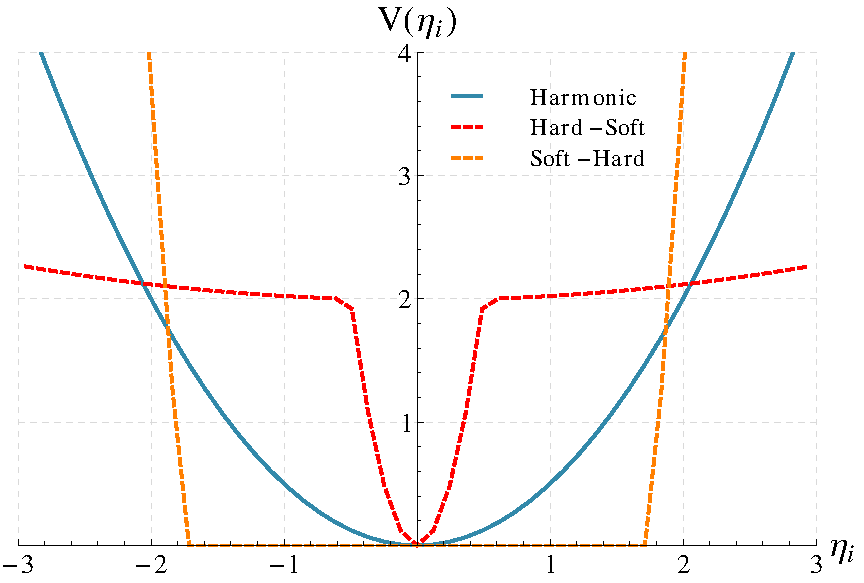
\includegraphics[scale=0.55]{Results/Collagen/various_potentials/col_pe_N5_L6_m24_kappa1_sigma1.pdf}
\caption{A potential plot of the harmonic potential and two anharmonic potentials. The potentials are a function of residue pair separations $(x_{i}-y_{i})$, $(x_{i}-z_{i})$ and $(z_{i}-y_{i})$ which we have labelled $\eta_{i}$.  }
\label{fig:collagen_pe}
\end{figure}

\begin{figure}[H]
\centering 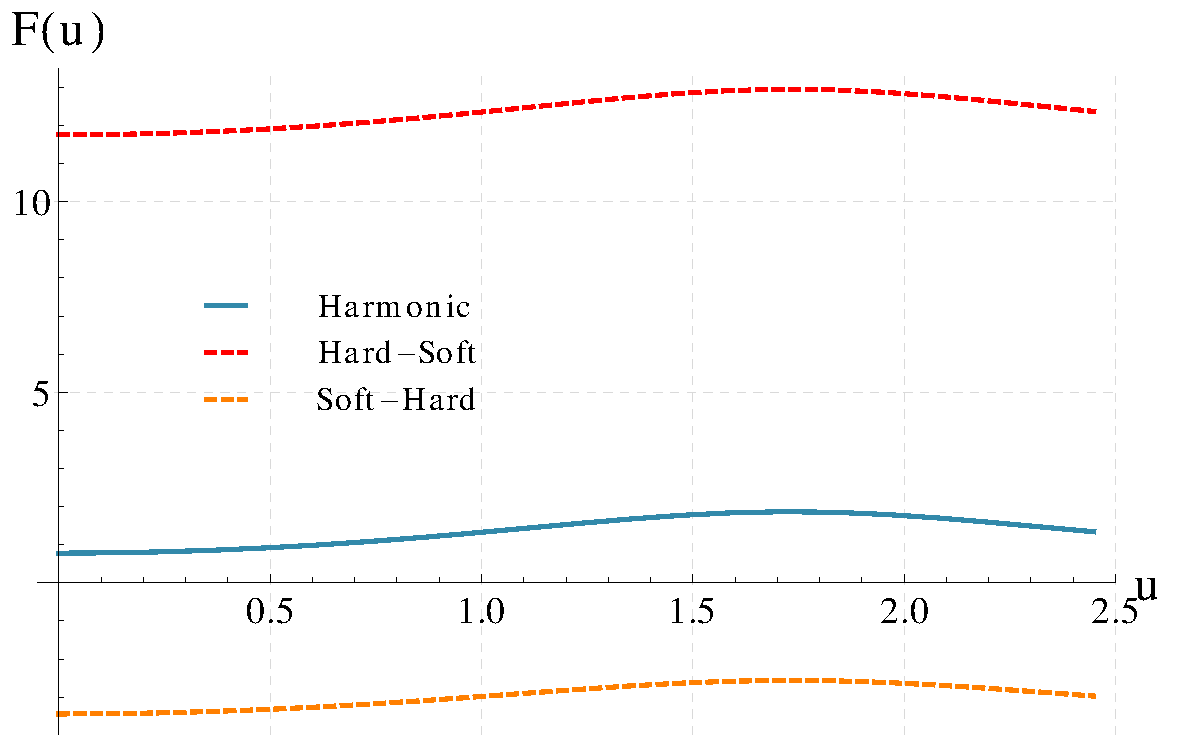
\includegraphics[scale=0.4]{Results/Collagen/various_potentials/col_fe_N5_L6_m24_kappa1_sigma1.pdf}
\caption{A plot of the resulting free energy calculations of the various potentials.}
\label{fig:collagen_fe}
\end{figure}

\begin{figure}[H]
\centering 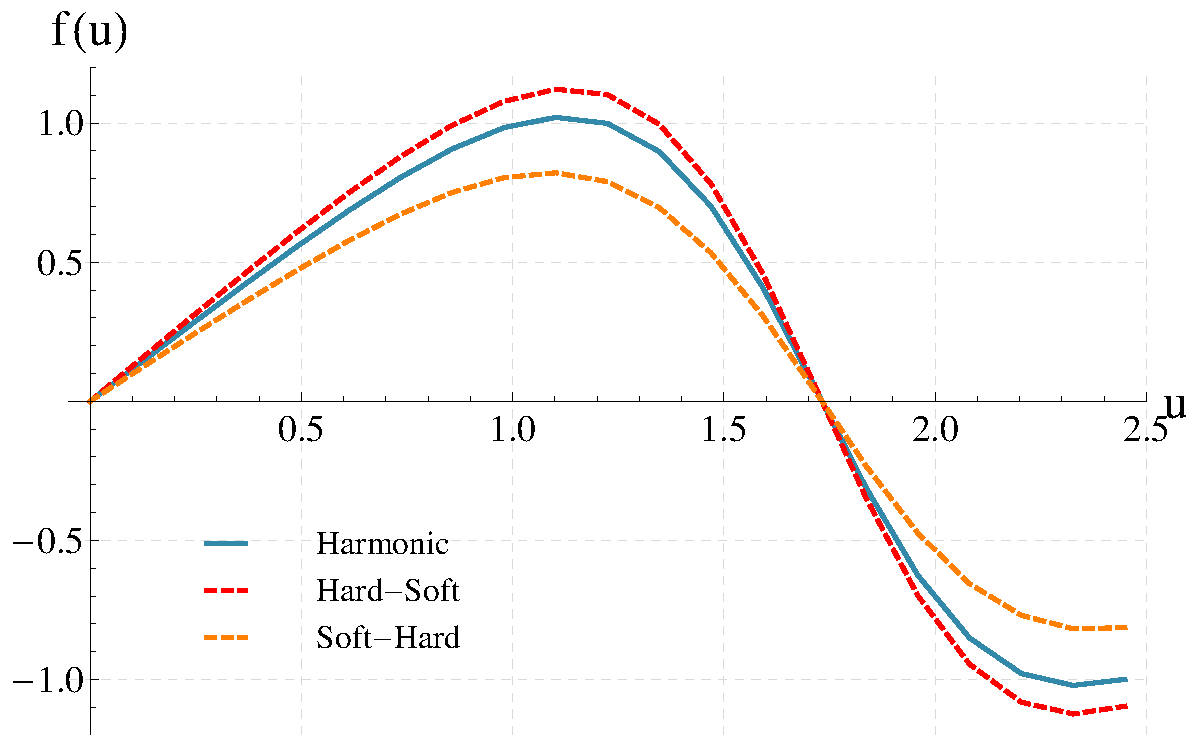
\includegraphics[scale=0.4]{Results/Collagen/various_potentials/col_dfe_N5_L6_m24_kappa1_sigma1.pdf}
\caption{The force-extension plots for the various potentials clearly show the effects of the transitions in the two anharmonic potentials. We include the force-extension of the harmonic potential that has a constant restoring force for an applied extension.}
\label{fig:collagen_dfe}
\end{figure}

\begin{figure}[H]
\centering
\begin{tabular}{cc}
\subfloat[Harmonic]{\label{fig:col_mxd_har}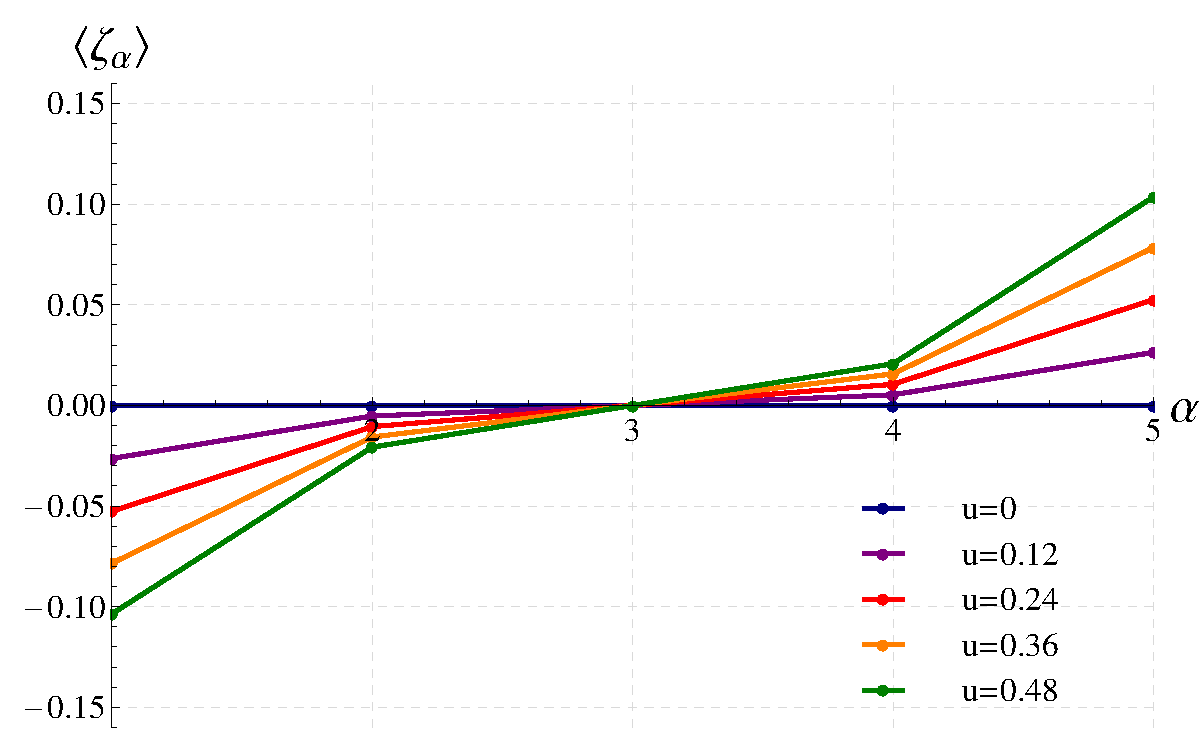
\includegraphics[scale=0.5]{Results/Collagen/various_potentials/harmonic/col_mxd_har_N5_L6_m24_kappa1_sigma1.pdf}} \\
\subfloat[Anharmonic 1 - Hard-to-Soft]{\label{fig:col_mxd_hard_soft}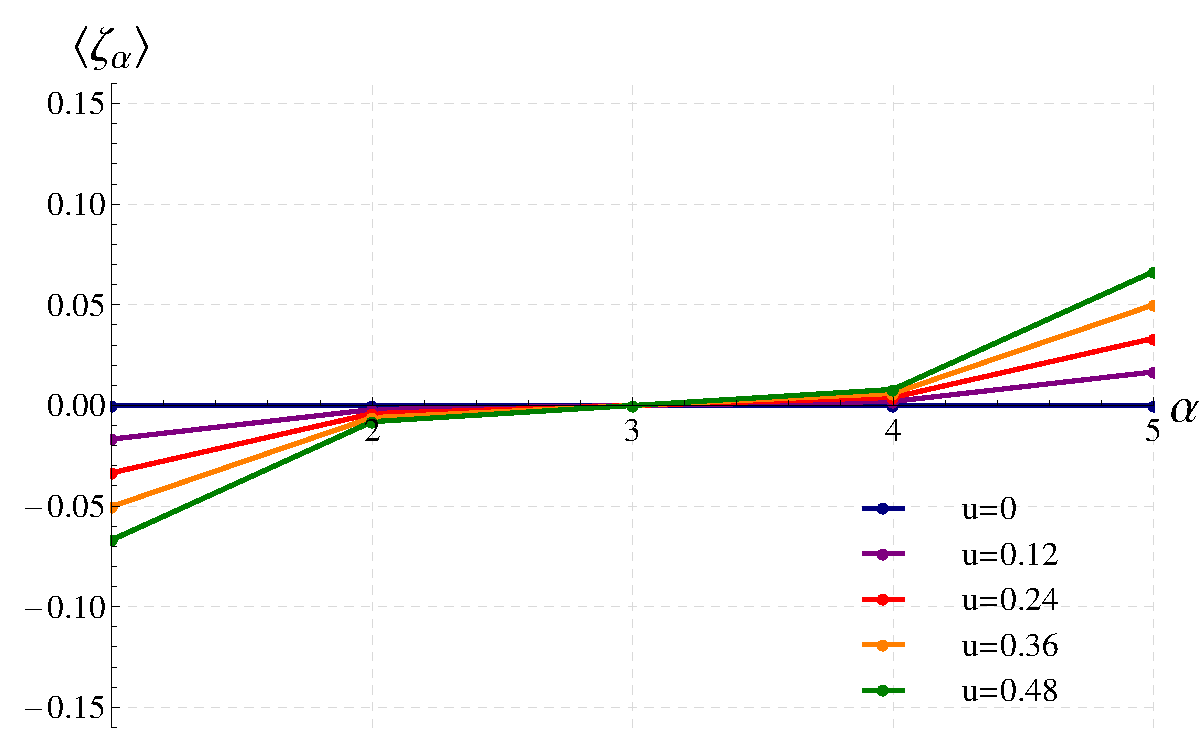
\includegraphics[scale=0.5]{Results/Collagen/various_potentials/hard_soft/col_mxd_hard_soft_N5_L6_m24_kappa1_sigma1.pdf}} \\
\subfloat[Anharmonic 2 - Soft-to-Hard]{\label{fig:col_mxd_soft_hard}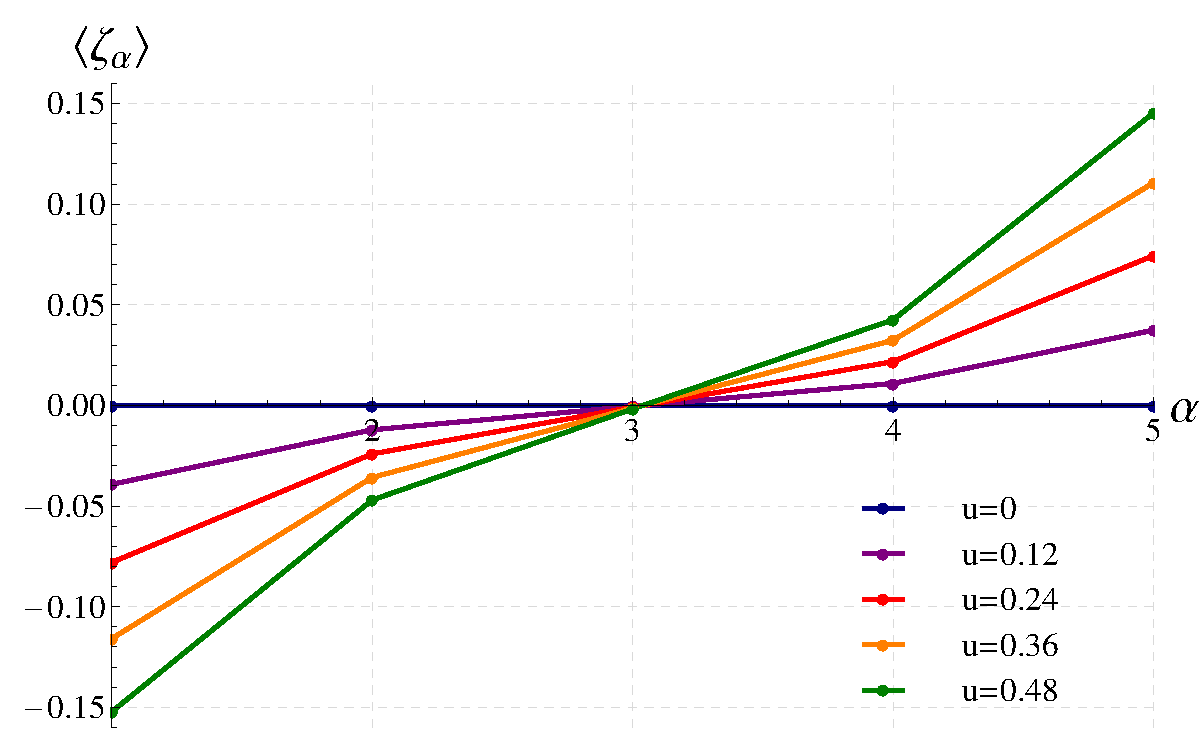
\includegraphics[scale=0.5]{Results/Collagen/various_potentials/soft_hard/col_mxd_soft_hard_N5_L6_m24_kappa1_sigma1.pdf}} 
\end{tabular}
\caption{Mean axial displacement plots for the Harmonic, Soft-to-Hard and Hard-to-Soft potentials up to an extension of $u=0.48$. Unlike DNA where the mean axial displacement is the average separation of the base-pair, in collagen it is the average separation of adjacent residue triplets given by \eqref{col_mxd2}.}
\label{fig:col_mxd}
\end{figure}

\section{Results for collagen calculations}

Starting from the same potential to model the base pairs in DNA, we adjust the stiffness to take into account only a single hydrogen bond between a residue pair in collagen. Reducing the spring constant by a factor of 2.5 we determine $\kappa' \approx 2.7 \times 10^{-4}\text{ eV/\AA}^{2}$.

Several views can be taken to determine the backbone spring constant of collagen. The simplest case is to view the collagen backbone as a collection of covalent bonds identical to DNA and this gives $\kappa/\kappa' \approx 370$. MD simulations in \cite{Buehler2007} provided data for backbone stretching in phase II of the force-extension plot \figref{buehler_model} which we are able to use to fit the backbone spring constant in our model. Since these MD simulations had constraints applied to each of the three carbon atoms at the ends of the collagen molecule, in our coarse-grained structure, we calculated a backbone spring constant of $\kappa \approx 6 \text{ eV/\AA}^{2}$. This gave an extremely high ratio of $\kappa/\kappa' \approx 22300$.

Atomistic calculations on a single polypeptide molecule using a reactive force field gave a backbone spring constant of $\kappa \approx 1.2 \text{ eV/\AA}^{2}$ \cite{Buehler2006} and a more accurate estimation of the backbone spring constant using MD simulations was calculated by the extended MARTINI force-field to give $\kappa \approx 0.16 \text{ eV/\AA}^{2}$ \cite{Gautieri2010}. This value fits much closer to the backbone stiffness of DNA used by Prakash et al. as well as giving a more reasonable backbone to residue pair stiffness ratio of $\kappa/\kappa' \approx 500$ for collagen.

With the known quantities of the backbone and residue pair stiffness constants we attempt to reproduce shearing force data for different molecular lengths of collagen. Using a method employed by Prakash et al. \cite{Prakash2011}, we determine the shear force $f_{s}$ when the separation of the end $xz$ residue pairs in the structure, $\eta_1$ and $\eta_N$, is equal to our fitting parameter $\eta_{B}$. We express $\eta$ as follows
%
\begin{equation}
\eta_{i}=x_{i}-z_{i}
\end{equation}
%
where $i$ refers to the index of the residue triplet. This is also known as the shearing separation of a residue pair. To simplify the calculation we use a harmonic approximation of Prakash's base pair potential for the residue pairs; this allows us to use the semi-analytical expression of the partition function. Setting the shearing distance of a single hydrogen bond $\eta_{B}$ to be around 2-3 \AA, we calculate the shear forces against molecular lengths for various backbone spring constants \figref{collagen_results}. The results clearly demonstrate the relationship between larger shearing forces and the increase in the backbone stiffness. It is understood that for a given extension, a larger $\kappa$ increases the amount of energy required to shear the molecule, thus increasing the shear force.

In comparing \figref{collagen_a} to \figref{collagen_c} we observe clearly that the breakage becomes insensitive to the length of the molecule, suggesting that the distortion only penetrates a certain distance into the structure from the ends of at the extension where failure occurs. By increasing $\kappa$ we increase the stiffness ratio between the residue pair and the backbone $\kappa/\kappa'$ allowing more energy to be stored in the residue pairs. This increases the penetrating length of distortions within the molecular structure at an applied extension.

The results shown in \figref{collagen_a} are considered to be a reasonable prediction of the response of to the collagen molecule. Though no experimental studies have been done to give the relationship between the molecular length and shearing force we  find that the backbone stiffness constant, and the backbone residue pair stiffness ratio, are within a reasonable estimates and compatible with what we have learned from studies of DNA. Compared to DNA other values of $\kappa$ were very large and gave extremely high $\kappa/\kappa'$ ratios.

\begin{figure}[H]
\centering
\begin{tabular}{cc}
\subfloat[$\kappa = 0.12 \text{ eV/\AA}^{2}$]{\label{fig:collagen_a}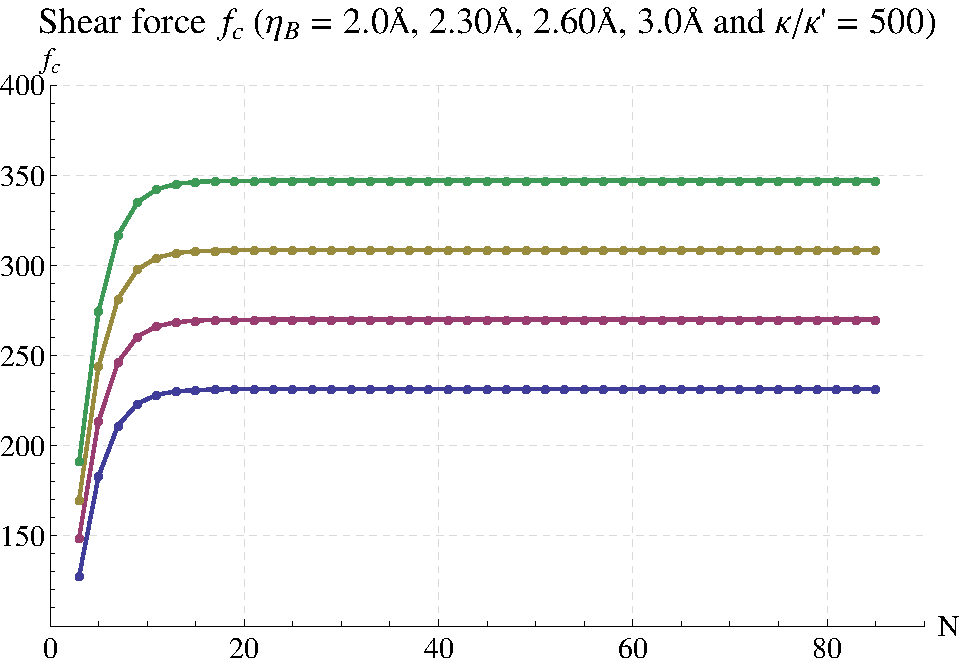
\includegraphics[scale=0.55]{Results/Collagen/shear_force_ksr500.pdf}} \\
\subfloat[$\kappa = 1.20 \text{ eV/\AA}^{2}$]{\label{fig:collagen_b}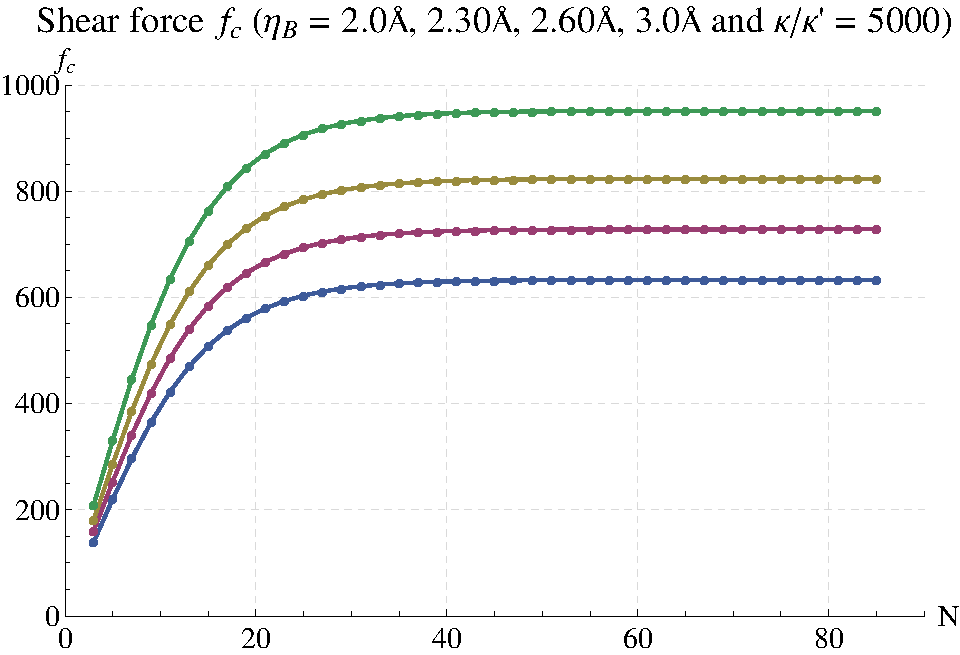
\includegraphics[scale=0.55]{Results/Collagen/shear_force_ksr5000.pdf}} \\
\subfloat[$\kappa = 6.00 \text{ eV/\AA}^{2}$]{\label{fig:collagen_c}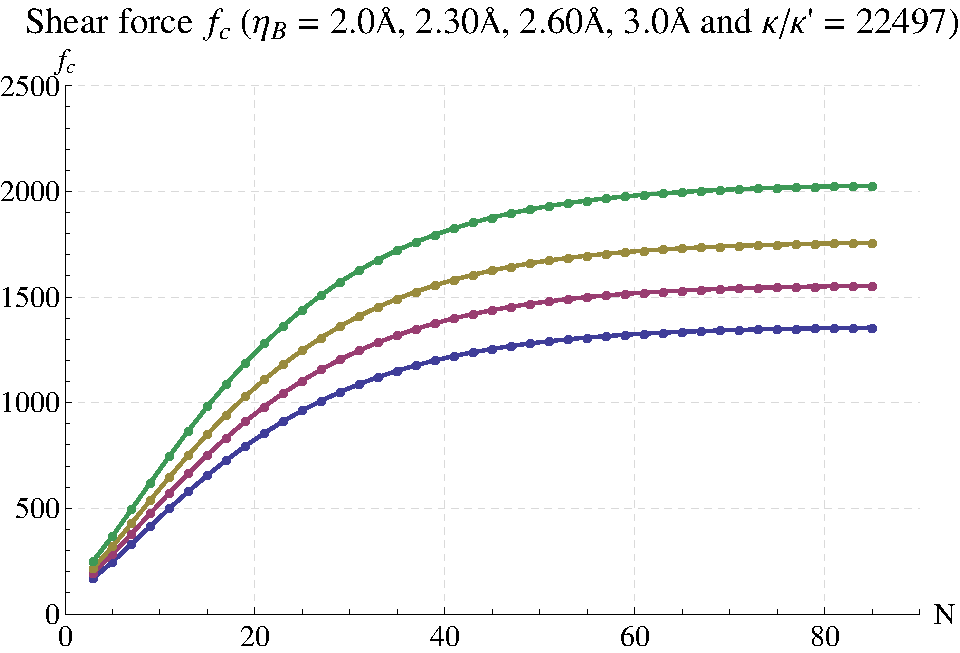
\includegraphics[scale=0.55]{Results/Collagen/shear_force_ksr22500.pdf}} 
\end{tabular}
\caption{Calculations of the shear force against molecular length. In each plot we determine the shear force curve for different $\eta_{B}$ values having the range between 2-3\AA.  The results for three different values of $\kappa$ are shown in \figref{collagen_a}, \figref{collagen_b} and \figref{collagen_c}.}
\label{fig:collagen_results} 
\end{figure}
